% Template:     Informe/Reporte LaTeX
% Documento:    Archivo principal
% Versión:      6.4.4 (13/08/2019)
% Codificación: UTF-8
%
% Autor: Pablo Pizarro R. @ppizarror
%        Facultad de Ciencias Físicas y Matemáticas
%        Universidad de Chile
%        pablo.pizarro@ing.uchile.cl, ppizarror.com
%
% Manual template: [https://latex.ppizarror.com/Template-Informe/]
% Licencia MIT:    [https://opensource.org/licenses/MIT/]

% CREACIÓN DEL DOCUMENTO
\documentclass[letterpaper,11pt]{article} % Articulo tamaño carta, 11pt
\usepackage[utf8]{inputenc} % Codificación UTF-8
\usepackage{graphics}
\usepackage{graphicx}
\usepackage{enumerate}
\usepackage{subfig}
\usepackage{multicol}
\usepackage{fancyvrb}
\usepackage{multirow}
\usepackage{mathtools}
%\usepackage{subcaption}

\graphicspath{ {C:\Users\EO\Dropbox\PDF\Ramos\Control adaptativo\Tareas\Tarea 1\Template-Informe-ext\img} }

% INFORMACIÓN DEL DOCUMENTO
\def\titulodelinforme {Ejercicio N° 2}
\def\temaatratar {Control adaptativo de sistemas}

\def\autordeldocumento {Elías Obreque Sepúlveda}
\def\nombredelcurso {}
\def\codigodelcurso {EL-7017}

\def\nombreuniversidad {Universidad de Chile}
\def\nombrefacultad {Facultad de Ciencias Físicas y Matemáticas}
\def\departamentouniversidad {Departamento de Ingeniería Eléctrica}
\def\imagendepartamento {departamentos/fcfm}
\def\imagendepartamentoescala {0.2}
\def\localizacionuniversidad {Santiago, Chile}


% INTEGRANTES, PROFESORES Y FECHAS
\def\tablaintegrantes {
\begin{tabular}{ll}
	Integrantes:
	& \begin{tabular}[t]{l}
		Elías Obreque
	\end{tabular} \\
	Profesor:
	& \begin{tabular}[t]{l}
		Manuel Duarte
	\end{tabular} \\
	Auxiliar:
	& \begin{tabular}[t]{l}
		Lisbel Bárzaga
	\end{tabular} \\
	& \\
	\multicolumn{2}{l}{Fecha de realización: \today} \\
	\multicolumn{2}{l}{Fecha de entrega: \today} \\
	\multicolumn{2}{l}{\localizacionuniversidad}
\end{tabular}}{
}

% CONFIGURACIONES
% Template:     Informe/Reporte LaTeX
% Documento:    Configuraciones del template
% Versión:      6.4.4 (13/08/2019)
% Codificación: UTF-8
%
% Autor: Pablo Pizarro R. @ppizarror
%        Facultad de Ciencias Físicas y Matemáticas
%        Universidad de Chile
%        pablo.pizarro@ing.uchile.cl, ppizarror.com
%
% Manual template: [https://latex.ppizarror.com/Template-Informe/]
% Licencia MIT:    [https://opensource.org/licenses/MIT/]

% CONFIGURACIONES GENERALES
\def\addemptypagetwosides {false}  % Añade pag en blanco al imprimir a 2 caras
\def\defaultinterline {1.0}        % Interlineado por defecto [pt]
\def\defaultnewlinesize {11}       % Tamaño del salto de línea [pt]
\def\documentlang {es-CL}          % Define el idioma del documento
\def\fontdocument {lmodern}        % Tipografía base, ver soportadas en manual
\def\fonttypewriter {tmodern}      % Tipografía de \texttt, ver manual online
\def\fonturl {tt}                  % Tipo de fuente url {tt,sf,rm,same}
\def\importtikz {false}            % Utilizar la librería tikz
\def\pointdecimal {true}           % N° decimales con punto en vez de coma
\def\predocpageromannumber {true}  % Pág. con número romano previo a inicio doc.
\def\predocpageromanupper {false}  % Páginas en número romano en mayúsculas
\def\predocresetpagenumber {true}  % Resetea número de la pag. tras el índice
\def\showlinenumbers {false}       % Muestra los números de línea del documento

% ESTILO PORTADA Y HEADER-FOOTER
\def\disablehfrightmark {false}    % Desactiva el rightmark del header-footer
\def\hfstyle {style1}              % Estilo header-footer (16 estilos)
\def\hfwidthcourse {0.35}          % Tamaño máximo del curso en header-footer
\def\hfwidthtitle {0.6}            % Tamaño máximo del título en header-footer
\def\hfwidthwrap {false}           % Activa el tamaño máximo en header-footer
\def\portraitstyle {style1}        % Estilo portada (20 estilos)

% CONFIGURACIÓN DE LAS LEYENDAS - CAPTION
\def\captionalignment {justified}  % Posición {centered,justified,left,right}
\def\captionlabelformat {simple}   % Formato leyenda {empty,simple,parens}
\def\captionlabelsep {colon}       % Sep. {none,colon,period,space,quad,newline}
\def\captionlessmarginimage {0.1}  % Margen sup/inf de fig. si no hay ley. [cm]
\def\captionlrmargin {2.0}         % Márgenes izq/der de la leyenda [cm]
\def\captionmarginmultimg {0.0}    % Margen izq/der leyendas múltiple img [cm]
\def\captionnumcode {arabic}       % N° código {arabic,alph,Alph,roman,Roman}
\def\captionnumequation {arabic}   % N° ecuaciones {arabic,alph,Alph,roman,Roman}
\def\captionnumfigure {arabic}     % N° figuras {arabic,alph,Alph,roman,Roman}
\def\captionnumsubfigure {alph}    % N° subfiguras {arabic,alph,Alph,roman,Roman}
\def\captionnumsubtable {alph}     % N° subtabla {arabic,alph,Alph,roman,Roman}
\def\captionnumtable {arabic}      % N° tabla {arabic,alph,Alph,roman,Roman}
\def\captiontbmarginfigure {9.35}  % Margen sup/inf de la leyenda en fig. [pt]
\def\captiontbmargintable {7.0}    % Margen sup/inf de la leyenda en tab. [pt]
\def\captiontextbold {false}       % Etiqueta (código,figura,tabla) en negrita
\def\captiontextsubnumbold {false} % N° subfigura/subtabla en negrita
\def\codecaptiontop {true}         % Leyenda arriba del código fuente
\def\figurecaptiontop {false}      % Leyenda arriba de las imágenes
\def\sectioncaptiondelimiter {.}   % Carácter delimitador N° objeto y sección
\def\showsectioncaptioncode {none} % N° sec. código {none,(s/ss/sss/ssss)ec}
\def\showsectioncaptioneqn {none}  % N° sec. ecuación {none,(s/ss/sss/ssss)ec}
\def\showsectioncaptionfig {none}  % N° sec. figuras {none,(s/ss/sss/ssss)ec}
\def\showsectioncaptiontab {none}  % N° sec. tablas {none,(s/ss/sss/ssss)ec}
\def\subcaptionlabelformat{parens} % Formato leyenda sub. {empty,simple,parens}
\def\subcaptionlabelsep {space}    % Sep. {none,colon,period,space,quad,newline}
\def\tablecaptiontop {true}        % Leyenda arriba de las tablas

% CONFIGURACIÓN DEL ÍNDICE
\def\charafterobjectindex {.}      % Carácter después de n° figura,tabla,código
\def\charnumpageindex {.}          % Carácter número de página en índice
\def\indexdepth {4}                % Profundidad máxima del índice
\def\indexnewpagec {false}         % Nueva página en índice códigos fuente
\def\indexnewpagef {false}         % Nueva página en índice figuras
\def\indexnewpaget {false}         % Nueva página en índice tablas
\def\indexstyle {ftc}              % Estilo índice {f:figura, t:tabla, c:código}
\def\indextitlemargin {11.4}       % Margen título índice \insertindextitle [pt]
\def\objectindexindent {false}     % Indenta la lista de objetos
\def\showindex {true}              % Muestra el índice
\def\showindexofcontents {true}    % Muestra la lista de contenidos

% ANEXO, CITAS, REFERENCIAS
\def\apaciterefsep {9}             % Separación entre refs. {apacite} [pt]
\def\appendixindepobjnum {true}    % Anexo usa n° objetos independientes
\def\bibtexrefsep {5}              % Separación entre refs. {bibtex} [pt]
\def\natbibrefsep {5}              % Separación entre referencia {natbib} [pt]
\def\natbibrefstyle {ieeetr}       % Formato de ref. natbib {apa,ieeetr,etc...}
\def\sectionappendixlastchar {.}   % Carácter entre n° de sec. anexo y título
\def\sectionrefenv {false}         % Las referencias se consideran como sección
\def\showappendixsecindex {true}   % Título de la sec. de anexos en el índice
\def\stylecitereferences {bibtex}  % Estilo cita/ref. {apacite,bibtex,natbib}
\def\twocolumnreferences {false}   % Referencias en dos columnas

% CONFIGURACIONES DE OBJETOS
\def\columnhspace {-0.4}           % Margen horizontal entre obj. \createcolumn
\def\columnsepwidth {2.1}          % Separación entre columnas [em]
\def\defaultimagefolder {img/}     % Carpeta raíz de las imágenes
\def\equationleftalign {false}     % Ecuaciones alineadas a la izquierda
\def\equationrestart {sec}         % Reinicio n° ecuac. {none,(s/ss/sss/ssss)ec}
\def\footnotepagetoprule {false}   % Footnote en pag. tienen separador superior
\def\footnoterestart {none}        % N° footnote {none,page,(s/ss/sss/ssss)ec}
\def\imagedefaultplacement {H}     % Posición por defecto de las imágenes
\def\marginalignbottom {-0.30}     % Margen inferior entorno align [cm]
\def\marginaligncaptbottom {0.05}  % Margen inferior entorno align caption[cm]
\def\marginaligncapttop {-0.60}    % Margen superior entorno align caption [cm]
\def\marginalignedbottom {-0.30}   % Margen inferior entorno aligned [cm]
\def\marginalignedcaptbottom {0.0} % Margen inferior entorno aligned caption[cm]
\def\marginalignedcapttop {-0.60}  % Margen superior entorno aligned caption[cm]
\def\marginalignedtop {-0.40}      % Margen superior entorno aligned [cm]
\def\marginaligntop {-0.40}        % Margen superior entorno align [cm]
\def\margineqncaptionbottom {0.0}  % Margen inferior caption ecuación [cm]
\def\margineqncaptiontop {-0.65}   % Margen superior caption ecuación [cm]
\def\marginequationbottom {-0.15}  % Margen inferior ecuaciones [cm]
\def\marginequationtop {0.0}       % Margen superior ecuaciones [cm]
\def\marginfloatimages {-13.0}     % Margen sup. fig. insertimageleft/right [pt]
\def\marginfootnote {10.0}         % Margen derecho footnote [pt]
\def\margingatherbottom {-0.20}    % Margen inferior entorno gather [cm]
\def\margingathercaptbottom {0.05} % Margen inferior entorno gather caption [cm]
\def\margingathercapttop {-0.77}   % Margen superior entorno gather [cm]
\def\margingatheredbottom {-0.10}  % Margen inf. entorno gathered [cm]
\def\margingatheredcaptbottom{0.0} % Margen inf. entorno gathered caption [cm]
\def\margingatheredcapttop {-0.77} % Margen superior entorno gathered [cm]
\def\margingatheredtop {-0.40}     % Margen superior entorno gathered [cm]
\def\margingathertop {-0.40}       % Margen superior entorno gather [cm]
\def\marginimagebottom {-0.15}     % Margen inferior figura [cm]
\def\marginimagemultright {0.50}   % Margen derecho imágenes múltiples [cm]
\def\marginimagemulttop {-0.30}    % Margen superior imágenes múltiples [cm]
\def\marginimagetop {0.0}          % Margen superior figuras [cm]
\def\numberedequation {true}       % Ecuaciones con \insert... numeradas
\def\sourcecodefontf {\ttfamily}   % Tipo de letra código fuente
\def\sourcecodefonts {\small}      % Tamaño letra código fuente
\def\sourcecodenumbersep {6}       % Separación entre número línea y código [pt]
\def\sourcecodetabsize {3}         % Tamaño tabulación código fuente
\def\tabledefaultplacement {H}     % Posición por defecto de las tablas
\def\tablepaddingh {0.85}          % Espaciado horizontal de celda de las tablas
\def\tablepaddingv {1.05}          % Espaciado vertical de celda de las tablas
\def\tikzdefaultplacement {H}      % Posición por defecto de las figuras tikz

% CONFIGURACIÓN DE LOS TÍTULOS
\def\anumsecaddtocounter {false}   % Insertar títulos anum. aumenta n° de sec
\def\fontsizessstitle{\normalsize} % Tamaño sub-sub-subtítulos
\def\fontsizesubsubtitle {\large}  % Tamaño sub-subtítulos
\def\fontsizesubtitle {\Large}     % Tamaño subtítulos
\def\fontsizetitle {\LARGE}        % Tamaño títulos
\def\fontsizetitlei {\LARGE}       % Tamaño títulos en el índice
\def\showdotaftersnum {true}       % Punto al final de n° (s/ss/sss/ssss)ection
\def\stylessstitle {\bfseries}     % Estilo sub-sub-subtítulos
\def\stylesubsubtitle {\bfseries}  % Estilo sub-subtítulos
\def\stylesubtitle {\bfseries}     % Estilo subtítulos
\def\styletitle {\bfseries}        % Estilo títulos
\def\styletitlei {\bfseries}       % Estilo títulos en el índice

% CONFIGURACIÓN DE LOS COLORES DEL DOCUMENTO
\def\captioncolor {black}          % Color de la leyenda (código,figura,tabla)
\def\captiontextcolor {black}      % Color de la leyenda
\def\colorpage {white}             % Color de la página
\def\highlightcolor {yellow}       % Color del subrayado con \hl
\def\indextitlecolor {black}       % Color de los títulos del índice
\def\linenumbercolor {gray}        % Color del n° de línea (\showlinenumbers)
\def\linkcolor {black}             % Color de los links del documento
\def\maintextcolor {black}         % Color principal del texto
\def\numcitecolor {black}          % Color del n° de las referencias o citas
\def\portraittitlecolor {black}    % Color de los títulos de la portada
\def\showborderonlinks {false}     % Color de un link por un recuadro de color
\def\sourcecodebgcolor {lgray}     % Color de fondo del código fuente
\def\ssstitlecolor {black}         % Color de los sub-sub-subtítulos
\def\subsubtitlecolor {black}      % Color de los sub-subtítulos
\def\subtitlecolor {black}         % Color de los subtítulos
\def\tablelinecolor {black}        % Color de las líneas de las tablas
\def\tablerowfirstcolor {none}     % Primer color de celda de las tablas
\def\tablerowsecondcolor {gray!20} % Segundo color de celda de las tablas
\def\titlecolor {black}            % Color de los títulos
\def\urlcolor {magenta}            % Color de los enlaces web (\href,\url)

% MÁRGENES DE PÁGINA
\def\firstpagemargintop {3.8}      % Margen superior página portada [cm]
\def\pagemarginbottom {2.7}        % Margen inferior página [cm]
\def\pagemarginleft {2.54}         % Margen izquierdo página [cm]
\def\pagemarginright {2.54}        % Margen derecho página [cm]
\def\pagemargintop {3.0}           % Margen superior página [cm]

% OPCIONES DEL PDF COMPILADO
\def\addindextobookmarks {false}   % Añade el índice a los marcadores del pdf
\def\cfgbookmarksopenlevel {1}     % Nivel marcadores en pdf (1:secciones)
\def\cfgpdfbookmarkopen {true}     % Expande marcadores del nivel configurado
\def\cfgpdfcenterwindow {true}     % Centra ventana del lector al abrir el pdf
\def\cfgpdfcopyright {}            % Establece el copyright del documento
\def\cfgpdfdisplaydoctitle {true}  % Muestra título del informe en visor
\def\cfgpdffitwindow {false}       % Ajusta la ventana del lector tamaño pdf
\def\cfgpdfmenubar {true}          % Muestra el menú del lector
\def\cfgpdfpagemode {OneColumn}    % Modo de página {OneColumn,SinglePage}
\def\cfgpdfpageview {FitH}         % {Fit,FitH,FitV,FitR,FitB,FitBH,FitBV}
\def\cfgpdfsecnumbookmarks {true}  % Número de la sec. en marcadores del pdf
\def\cfgpdftoolbar {true}          % Muestra barra de herramientas lector pdf
\def\cfgshowbookmarkmenu {false}   % Muestra menú marcadores al abrir el pdf
\def\pdfcompilecompression {9}     % Factor de compresión del pdf (0-9)
\def\pdfcompileobjcompression {2}  % Nivel compresión objetos del pdf (0-3)
\def\pdfcompileversion {7}         % Versión mínima del pdf compilado

% NOMBRE DE OBJETOS
\def\nameabstract {Resumen}           % Nombre del resumen-abstract
\def\nameappendixsection {Anexos}     % Nombre de la sec. de anexos/apéndices
\def\nameportraitpage {Portada}       % Etiqueta página de la portada
\def\namereferences {Referencias}     % Nombre de la sección de referencias
\def\nomchapter {Capítulo}            % Nombre de los capítulos
\def\nomltappendixsection {Anexo}     % Etiqueta sección en anexo/apéndices
\def\nomltcont {Índice de Contenidos} % Nombre del índice de contenidos
\def\nomltfigure {Índice de Figuras}  % Nombre del índice de lista de figuras
\def\nomltsrc {Índice de Códigos}     % Nombre del índice de lista de código
\def\nomlttable {Índice de Tablas}    % Nombre del índice de lista de tablas
\def\nomltwfigure {Figura}            % Etiqueta leyenda de las figuras
\def\nomltwsrc {Código}               % Etiqueta leyenda del código fuente
\def\nomltwtable {Tabla}              % Etiqueta leyenda de las tablas
\def\nomnpageof { de }                % Etiqueta página # de #


% IMPORTACIÓN DE LIBRERÍAS
% Template:     Informe/Reporte LaTeX
% Documento:    Importación de librerías
% Versión:      6.4.4 (13/08/2019)
% Codificación: UTF-8
%
% Autor: Pablo Pizarro R. @ppizarror
%        Facultad de Ciencias Físicas y Matemáticas
%        Universidad de Chile
%        pablo.pizarro@ing.uchile.cl, ppizarror.com
%
% Manual template: [https://latex.ppizarror.com/Template-Informe/]
% Licencia MIT:    [https://opensource.org/licenses/MIT/]

\usepackage[spanish,es-nosectiondot,es-lcroman,es-noquoting]{babel}
\usepackage{ifthen}
\newcommand{\throwbadconfig}[4][]{
	\ifthenelse{\equal{#1}{noheader}}{
		\errmessage{LaTeX Warning: #4}
	}{
		\ifthenelse{\equal{#1}{noheader-nostop}}{
			\errmessage{LaTeX Warning: #4}
		}{
			\errmessage{LaTeX Warning: #2 \noexpand #3=#3. Valores esperados: #4}
		}
	}
	\ifthenelse{\equal{#1}{nostop}}{}{
		\ifthenelse{\equal{#1}{noheader-nostop}}{}{
			\stop
		}
	}
}
\ifthenelse{\equal{\equationleftalign}{true}}{
	\usepackage[fleqn]{amsmath}
}{
	\usepackage{amsmath}
}
\let\counterwithout\relax
\let\counterwithin\relax
\let\RE\Re
\let\IM\Im
\usepackage{amssymb}
\usepackage{array}
\usepackage{bigstrut}
\usepackage{bm}
\usepackage{booktabs}
\usepackage{caption}
\usepackage{changepage}
\usepackage{chngcntr}
\usepackage{color}
\usepackage{datetime}
\usepackage{floatpag}
\usepackage{floatrow}
\usepackage{framed}
\usepackage{gensymb}
\usepackage{geometry}
\usepackage{graphicx}
\usepackage{lipsum}
\usepackage{listings}
\usepackage{listingsutf8}
\usepackage{longtable}
\usepackage{mathtools}
\usepackage{multicol}
\usepackage{needspace}
\usepackage{pdflscape}
\usepackage{pdfpages}
\usepackage{physics}
\usepackage{rotating}
\usepackage{sectsty}
\usepackage{selinput}
\usepackage{setspace}
\usepackage{soul}
\usepackage{subfig}
\usepackage{textcomp}
\usepackage{url}
\usepackage{wasysym}
\usepackage{wrapfig}
\usepackage{xspace}
\usepackage[makeroom]{cancel}
\usepackage[inline]{enumitem}
\usepackage[subfigure,titles]{tocloft}
\usepackage[figure,table,lstlisting]{totalcount}
\usepackage[normalem]{ulem}
\usepackage[dvipsnames,table,usenames]{xcolor}
\ifthenelse{\equal{\footnotepagetoprule}{true}}{
\usepackage[bottom,hang]{footmisc}
}{
	\usepackage[bottom,norule,hang]{footmisc}
}
\ifthenelse{\equal{\showdotaftersnum}{true}}{
	\usepackage{secdot}
	\sectiondot{subsection}
	\sectiondot{subsubsection}}{
}
\ifthenelse{\equal{\stylecitereferences}{natbib}}{
	\ifthenelse{\equal{\natbibrefstyle}{apa}}{
		\usepackage{natbib}
	}{
	\ifthenelse{\equal{\natbibrefstyle}{ieeetr}}{
		\usepackage[numbers]{natbib}
	}{
	\ifthenelse{\equal{\natbibrefstyle}{unsrt}}{
		\usepackage[numbers]{natbib}
	}{
	\ifthenelse{\equal{\natbibrefstyle}{abbrvnat}}{
		\usepackage[numbers]{natbib}
	}{
		\usepackage{natbib}
	}}}}
}{
\ifthenelse{\equal{\stylecitereferences}{apacite}}{
		\usepackage{apacite}
	}{
\ifthenelse{\equal{\stylecitereferences}{bibtex}}{
		}{}
	}
}
\ifthenelse{\equal{\showappendixsecindex}{true}}{
	\usepackage[toc]{appendix}
}{
	\usepackage{appendix}
}
\ifthenelse{\equal{\importtikz}{true}}{
	\usepackage{tikz}}{
}
\usepackage[pdfencoding=auto,psdextra]{hyperref}
\ifthenelse{\equal{\hfstyle}{style11}}{
	\usepackage{lastpage}}{}
\ifthenelse{\equal{\hfstyle}{style12}}{
	\usepackage{lastpage}}{}
\ifthenelse{\equal{\hfstyle}{style13}}{
	\usepackage{lastpage}}{}
\ifthenelse{\equal{\hfstyle}{style14}}{
	\usepackage{lastpage}}{
}
\usepackage{bookmark}
\usepackage{fancyhdr}
\usepackage{float}
\usepackage{hyperxmp}
\usepackage{multirow}
\usepackage{notoccite}
\usepackage{titlesec}
\ifthenelse{\equal{\fontdocument}{lmodern}}{
	\usepackage{lmodern}
}{
\ifthenelse{\equal{\fontdocument}{arial}}{
	\usepackage{helvet}
	\renewcommand{\familydefault}{\sfdefault}
}{
\ifthenelse{\equal{\fontdocument}{arial2}}{
	\usepackage{arial}
}{
\ifthenelse{\equal{\fontdocument}{times}}{
	\usepackage{mathptmx}
}{
\ifthenelse{\equal{\fontdocument}{helvet}}{
	\usepackage{helvet}
}{
\ifthenelse{\equal{\fontdocument}{alegreyasans}}{
	\usepackage[sfdefault]{AlegreyaSans}
	\renewcommand*\oldstylenums[1]{{\AlegreyaSansOsF #1}}
}{
\ifthenelse{\equal{\fontdocument}{mathpazo}}{
	\usepackage{mathpazo}
}{
\ifthenelse{\equal{\fontdocument}{accantis}}{
	\usepackage{accanthis}
}{
\ifthenelse{\equal{\fontdocument}{alegreya}}{
	\usepackage{Alegreya}
	\renewcommand*\oldstylenums[1]{{\AlegreyaOsF #1}}
}{
\ifthenelse{\equal{\fontdocument}{algolrevived}}{
	\usepackage{algolrevived}
}{
\ifthenelse{\equal{\fontdocument}{antiqua}}{
	\usepackage{antiqua}
}{
\ifthenelse{\equal{\fontdocument}{antpolt}}{
	\usepackage{antpolt}
}{
\ifthenelse{\equal{\fontdocument}{antpoltlight}}{
	\usepackage[light]{antpolt}
}{
\ifthenelse{\equal{\fontdocument}{anttor}}{
	\usepackage[math]{anttor}
}{
\ifthenelse{\equal{\fontdocument}{anttorcondensed}}{
	\usepackage[condensed,math]{anttor}
}{
\ifthenelse{\equal{\fontdocument}{anttorlight}}{
	\usepackage[light,math]{anttor}
}{
\ifthenelse{\equal{\fontdocument}{anttorlightcondensed}}{
	\usepackage[light,condensed,math]{anttor}
}{
\ifthenelse{\equal{\fontdocument}{arev}}{
	\usepackage{arev}
}{
\ifthenelse{\equal{\fontdocument}{arimo}}{
	\usepackage[sfdefault]{arimo}
	\renewcommand*\familydefault{\sfdefault}
}{
\ifthenelse{\equal{\fontdocument}{aurical}}{
	\usepackage{aurical}
}{
\ifthenelse{\equal{\fontdocument}{avant}}{
	\usepackage{avant}
}{
\ifthenelse{\equal{\fontdocument}{baskervald}}{
	\usepackage{baskervald}
}{
\ifthenelse{\equal{\fontdocument}{berasans}}{
	\usepackage[scaled]{berasans}
	\renewcommand*\familydefault{\sfdefault}
}{
\ifthenelse{\equal{\fontdocument}{beraserif}}{
	\usepackage{bera}
}{
\ifthenelse{\equal{\fontdocument}{biolinum}}{
	\usepackage{libertine}
	\renewcommand*\familydefault{\sfdefault}
}{
\ifthenelse{\equal{\fontdocument}{cabin}}{
	\usepackage[sfdefault]{cabin}
	\renewcommand*\familydefault{\sfdefault}
}{
\ifthenelse{\equal{\fontdocument}{cabincondensed}}{
	\usepackage[sfdefault,condensed]{cabin}
	\renewcommand*\familydefault{\sfdefault}
}{
\ifthenelse{\equal{\fontdocument}{cantarell}}{
	\usepackage[default]{cantarell}
}{
\ifthenelse{\equal{\fontdocument}{caladea}}{
	\usepackage{caladea}
}{
\ifthenelse{\equal{\fontdocument}{carlito}}{
	\usepackage[sfdefault]{carlito}
	\renewcommand*\familydefault{\sfdefault}
}{
\ifthenelse{\equal{\fontdocument}{chivolight}}{
	\usepackage[familydefault,light]{Chivo}
}{
\ifthenelse{\equal{\fontdocument}{chivoregular}}{
	\usepackage[familydefault,regular]{Chivo}
}{
\ifthenelse{\equal{\fontdocument}{clearsans}}{
	\usepackage[sfdefault]{ClearSans}
	\renewcommand*\familydefault{\sfdefault}
}{
\ifthenelse{\equal{\fontdocument}{comfortaa}}{
	\usepackage[default]{comfortaa}
}{
\ifthenelse{\equal{\fontdocument}{comicneue}}{
	\usepackage[default]{comicneue}
}{
\ifthenelse{\equal{\fontdocument}{comicneueangular}}{
	\usepackage[default,angular]{comicneue}
}{
\ifthenelse{\equal{\fontdocument}{crimson}}{
	\usepackage{crimson}
}{
\ifthenelse{\equal{\fontdocument}{cyklop}}{
	\usepackage{cyklop}
}{
\ifthenelse{\equal{\fontdocument}{dejavusans}}{
	\usepackage{DejaVuSans}
	\renewcommand*\familydefault{\sfdefault}
}{
\ifthenelse{\equal{\fontdocument}{dejavusanscondensed}}{
	\usepackage{DejaVuSansCondensed}
	\renewcommand*\familydefault{\sfdefault}
}{
\ifthenelse{\equal{\fontdocument}{droidsans}}{
	\usepackage[defaultsans]{droidsans}
	\renewcommand*\familydefault{\sfdefault}
}{
\ifthenelse{\equal{\fontdocument}{fetamont}}{
	\usepackage{fetamont}
	\renewcommand*\familydefault{\sfdefault}
}{
\ifthenelse{\equal{\fontdocument}{firasans}}{
	\usepackage[sfdefault]{FiraSans}
	\renewcommand*\familydefault{\sfdefault}
}{
\ifthenelse{\equal{\fontdocument}{iwona}}{
	\usepackage[math]{iwona}
}{
\ifthenelse{\equal{\fontdocument}{iwonacondensed}}{
	\usepackage[math]{iwona}
}{
\ifthenelse{\equal{\fontdocument}{iwonalight}}{
	\usepackage[light,math]{iwona}
}{
\ifthenelse{\equal{\fontdocument}{iwonalightcondensed}}{
	\usepackage[light,condensed,math]{iwona}
}{
\ifthenelse{\equal{\fontdocument}{kurier}}{
	\usepackage[math]{kurier}
}{
\ifthenelse{\equal{\fontdocument}{kuriercondensed}}{
	\usepackage[condensed,math]{kurier}
}{
\ifthenelse{\equal{\fontdocument}{kurierlight}}{
	\usepackage[light,math]{kurier}
}{
\ifthenelse{\equal{\fontdocument}{kurierlightcondensed}}{
	\usepackage[light,condensed,math]{kurier}
}{
\ifthenelse{\equal{\fontdocument}{lato}}{
	\usepackage[default]{lato}
}{
\ifthenelse{\equal{\fontdocument}{libris}}{
	\usepackage{libris}
	\renewcommand*\familydefault{\sfdefault}
}{
\ifthenelse{\equal{\fontdocument}{lxfonts}}{
	\usepackage{lxfonts}
}{
\ifthenelse{\equal{\fontdocument}{merriweather}}{
	\usepackage[sfdefault]{merriweather}
}{
\ifthenelse{\equal{\fontdocument}{merriweatherlight}}{
	\usepackage[sfdefault,light]{merriweather}
}{
\ifthenelse{\equal{\fontdocument}{mintspirit}}{
	\usepackage[default]{mintspirit}
}{
\ifthenelse{\equal{\fontdocument}{montserratalternatesextralight}}{
	\usepackage[defaultfam,extralight,tabular,lining,alternates]{montserrat}
	\renewcommand*\oldstylenums[1]{{\fontfamily{Montserrat-TOsF}\selectfont #1}}
}{
\ifthenelse{\equal{\fontdocument}{montserratalternatesregular}}{
	\usepackage[defaultfam,tabular,lining,alternates]{montserrat}
	\renewcommand*\oldstylenums[1]{{\fontfamily{Montserrat-TOsF}\selectfont #1}}
}{
\ifthenelse{\equal{\fontdocument}{montserratalternatesthin}}{
	\usepackage[defaultfam,thin,tabular,lining,alternates]{montserrat}
	\renewcommand*\oldstylenums[1]{{\fontfamily{Montserrat-TOsF}\selectfont #1}}
}{
\ifthenelse{\equal{\fontdocument}{montserratextralight}}{
	\usepackage[defaultfam,extralight,tabular,lining]{montserrat}
	\renewcommand*\oldstylenums[1]{{\fontfamily{Montserrat-TOsF}\selectfont #1}}
}{
\ifthenelse{\equal{\fontdocument}{montserratlight}}{
	\usepackage[defaultfam,light,tabular,lining]{montserrat}
	\renewcommand*\oldstylenums[1]{{\fontfamily{Montserrat-TOsF}\selectfont #1}}
}{
\ifthenelse{\equal{\fontdocument}{montserratregular}}{
	\usepackage[defaultfam,tabular,lining]{montserrat}
	\renewcommand*\oldstylenums[1]{{\fontfamily{Montserrat-TOsF}\selectfont #1}}
}{
\ifthenelse{\equal{\fontdocument}{montserratthin}}{
	\usepackage[defaultfam,thin,tabular,lining]{montserrat}
	\renewcommand*\oldstylenums[1]{{\fontfamily{Montserrat-TOsF}\selectfont #1}}
}{
\ifthenelse{\equal{\fontdocument}{nimbussans}}{
	\usepackage{nimbussans}
	\renewcommand*\familydefault{\sfdefault}
}{
\ifthenelse{\equal{\fontdocument}{noto}}{
	\usepackage[sfdefault]{noto}
	\renewcommand*\familydefault{\sfdefault}
}{
\ifthenelse{\equal{\fontdocument}{opensans}}{
	\usepackage[default,osfigures,scale=0.95]{opensans}
}{
\ifthenelse{\equal{\fontdocument}{overlock}}{
	\usepackage[sfdefault]{overlock}
	\renewcommand*\familydefault{\sfdefault}
}{
\ifthenelse{\equal{\fontdocument}{paratype}}{
	\usepackage{paratype}
	\renewcommand*\familydefault{\sfdefault}
}{
\ifthenelse{\equal{\fontdocument}{paratypesanscaption}}{
	\usepackage{PTSansCaption}
	\renewcommand*\familydefault{\sfdefault}
}{
\ifthenelse{\equal{\fontdocument}{paratypesansnarrow}}{
	\usepackage{PTSansNarrow}
	\renewcommand*\familydefault{\sfdefault}
}{
\ifthenelse{\equal{\fontdocument}{quattrocento}}{
	\usepackage[sfdefault]{quattrocento}
}{
\ifthenelse{\equal{\fontdocument}{raleway}}{
	\usepackage[default]{raleway}
}{
\ifthenelse{\equal{\fontdocument}{roboto}}{
	\usepackage[sfdefault]{roboto}
}{
\ifthenelse{\equal{\fontdocument}{robotocondensed}}{
	\usepackage[sfdefault,condensed]{roboto}
}{
\ifthenelse{\equal{\fontdocument}{robotolight}}{
	\usepackage[sfdefault,light]{roboto}
}{
\ifthenelse{\equal{\fontdocument}{robotolightcondensed}}{
	\usepackage[sfdefault,light,condensed]{roboto}
}{
\ifthenelse{\equal{\fontdocument}{robotothin}}{
	\usepackage[sfdefault,thin]{roboto}
}{
\ifthenelse{\equal{\fontdocument}{rosario}}{
	\usepackage[familydefault]{Rosario}
}{
\ifthenelse{\equal{\fontdocument}{sourcesanspro}}{
	\usepackage[default]{sourcesanspro}
}{
\ifthenelse{\equal{\fontdocument}{uarial}}{
	\usepackage{uarial}
	\renewcommand*\familydefault{\sfdefault}
}{
\ifthenelse{\equal{\fontdocument}{ugq}}{
	\renewcommand*\sfdefault{ugq}
	\renewcommand*\familydefault{\sfdefault}
}{
\ifthenelse{\equal{\fontdocument}{universalis}}{
	\usepackage[sfdefault]{universalis}
}{
\ifthenelse{\equal{\fontdocument}{universaliscondensed}}{
	\usepackage[condensed,sfdefault]{universalis}
}{
\ifthenelse{\equal{\fontdocument}{venturis}}{
	\usepackage[lf]{venturis}
	\renewcommand*\familydefault{\sfdefault}
}{
	\throwbadconfig[nostop]{Fuente desconocida}{\fontdocument}{(Fuentes clasicas) lmodern,arial,arial2,helvet,times,alegreyasans,mathpazo}
	\throwbadconfig[noheader-nostop]{Fuente desconocida}{\fontdocument}{(Fuentes adicionales) accantis,alegreya,algolrevived,antiqua,antpolt,antpoltlight,anttor,anttorcondensed,anttorlight,anttorlightcondensed,arev,arimo,aurical,avant,baskervald,berasans,beraserif,biolinum,cabin,cabincondensed,cantarell,caladea,carlito,chivolight,chivoregular,clearsans,comfortaa,comicneue,comicneueangular,crimson,cyklop,dejavusans,dejavusanscondensed,droidsans,firasans,iwona,iwonacondensed,iwonalight,iwonalightcondensed,kurier}
	\throwbadconfig[noheader-nostop]{Fuente desconocida}{\fontdocument}{kuriercondensed,kurierlight,kurierlightcondensed,lato,libris,lxfonts,merriweather,merriweatherlight,mintspirit,montserratalternatesextralight,montserratalternatesregular,montserratalternatesthin,montserratextralight,montserratlight,montserratregular,montserratthin,nimbussans,noto,opensans,overlock,paratype,paratypesanscaption,paratypesansnarrow,quattrocento,raleway,roboto,robotolight,robotolightcondensed,robotothin,rosario,sourcesanspro,uarial,ugq}
	\throwbadconfig[noheader]{Fuente desconocida}{\fontdocument}{universalis,universaliscondensed,venturis}
	}}}}}}}}}}}}}}}}}}}}}}}}}}}}}}}}}}}}}}}}}}}}}}}}}}}}}}}}}}}}}}}}}}}}}}}}}}}}}}}}}}}}
}
\ifthenelse{\equal{\fonttypewriter}{tmodern}}{
	\renewcommand*\ttdefault{lmvtt}
}{
\ifthenelse{\equal{\fonttypewriter}{anonymouspro}}{
	\usepackage[ttdefault=true]{AnonymousPro}
}{
\ifthenelse{\equal{\fonttypewriter}{ascii}}{
	\usepackage{ascii}
	\let\SI\relax
}{
\ifthenelse{\equal{\fonttypewriter}{beramono}}{
	\usepackage[scaled]{beramono}
}{
\ifthenelse{\equal{\fonttypewriter}{cmpica}}{
	\usepackage{addfont}
	\addfont{OT1}{cmpica}{\pica}
	\addfont{OT1}{cmpicab}{\picab}
	\addfont{OT1}{cmpicati}{\picati}
	\renewcommand*\ttdefault{pica}
}{
\ifthenelse{\equal{\fonttypewriter}{courier}}{
	\usepackage{courier}
}{
\ifthenelse{\equal{\fonttypewriter}{dejavusansmono}}{
	\usepackage[scaled]{DejaVuSansMono}
}{
\ifthenelse{\equal{\fonttypewriter}{firamono}}{
	\usepackage[scale=0.85]{FiraMono}
}{
\ifthenelse{\equal{\fonttypewriter}{gomono}}{
	\usepackage[scale=0.85]{GoMono}
}{
\ifthenelse{\equal{\fonttypewriter}{inconsolata}}{
	\usepackage{inconsolata}
}{
\ifthenelse{\equal{\fonttypewriter}{nimbusmono}}{
	\usepackage{nimbusmono}
}{
\ifthenelse{\equal{\fonttypewriter}{newtxtt}}{
	\usepackage[zerostyle=d]{newtxtt}
}{
\ifthenelse{\equal{\fonttypewriter}{nimbusmono}}{
	\usepackage{nimbusmono}
}{
\ifthenelse{\equal{\fonttypewriter}{nimbusmononarrow}}{
	\usepackage{nimbusmononarrow}
}{
\ifthenelse{\equal{\fonttypewriter}{lcmtt}}{
	\renewcommand*\ttdefault{lcmtt}
}{
\ifthenelse{\equal{\fonttypewriter}{sourcecodepro}}{
	\usepackage[ttdefault=true,scale=0.85]{sourcecodepro}
}{
\ifthenelse{\equal{\fonttypewriter}{texgyrecursor}}{
	\usepackage{tgcursor}
}{
	\throwbadconfig{Fuente desconocida}{\fonttypewriter}{anonymouspro,ascii,beramono,
		cmpica,courier,dejavusansmono,firamono,gomono,inconsolata,kpmonospaced,lcmtt,
		newtxtt,nimbusmono,nimbusmononarrow,texgyrecursor,tmodern}
	}}}}}}}}}}}}}}}}
}
\usepackage[T1]{fontenc}
\ifthenelse{\equal{\showlinenumbers}{true}}{
	\usepackage[switch,columnwise,running]{lineno}}{
}
\usepackage{csquotes}
\inputencoding{utf8}



% IMPORTACIÓN DE FUNCIONES Y ENTORNOS
% Template:     Informe/Reporte LaTeX
% Documento:    Carga las funciones del template
% Versión:      6.4.4 (13/08/2019)
% Codificación: UTF-8
%
% Autor: Pablo Pizarro R. @ppizarror
%        Facultad de Ciencias Físicas y Matemáticas
%        Universidad de Chile
%        pablo.pizarro@ing.uchile.cl, ppizarror.com
%
% Manual template: [https://latex.ppizarror.com/Template-Informe/]
% Licencia MIT:    [https://opensource.org/licenses/MIT/]

% Template:     Informe/Reporte LaTeX
% Documento:    Funciones del núcleo del template
% Versión:      6.4.4 (13/08/2019)
% Codificación: UTF-8
%
% Autor: Pablo Pizarro R. @ppizarror
%        Facultad de Ciencias Físicas y Matemáticas
%        Universidad de Chile
%        pablo.pizarro@ing.uchile.cl, ppizarror.com
%
% Manual template: [https://latex.ppizarror.com/Template-Informe/]
% Licencia MIT:    [https://opensource.org/licenses/MIT/]

\def\GLOBALcoretikzimported {false}
\def\GLOBALenvimageadded {false}
\def\GLOBALenvimageinitialized {false}
\def\GLOBALenvimagenewlinemarg {0.25}
\def\GLOBALsectionalph {false}
\def\GLOBALsectionanumenabled {false}
\def\GLOBALsubsectionanumenabled {false}
\def\GLOBALtablerowcolorindex {2}
\def\GLOBALtablerowcolorswitch {false}
\newcounter{templateEquations}
\newcounter{templateFigures}
\newcounter{templatePageCounter}
\newcounter{templateTables}
\newcounter{templateListings}
\newcommand{\throwerror}[2]{
	\errmessage{LaTeX Error: \noexpand#1 #2 (linea \the\inputlineno)}
	\stop
}
\newcommand{\throwwarning}[1]{
	\errmessage{LaTeX Warning: #1 (linea \the\inputlineno)}
}
\newcommand{\throwbadconfigondoc}[3]{
	\errmessage{#1 \noexpand #2=#2. Valores esperados: #3}
	\stop
}
\newcommand{\checkvardefined}[1]{
	\ifthenelse{\isundefined{#1}}{
		\errmessage{LaTeX Warning: Variable \noexpand#1 no definida}
		\stop}{
	}
}
\newcommand{\checkextravarexist}[2]{
	\ifthenelse{\isundefined{#1}}{
		\errmessage{LaTeX Warning: Variable \noexpand#1 no definida}
		\ifx\hfuzz#2\hfuzz
			\errmessage{LaTeX Warning: Defina la variable en el bloque de INFORMACION DEL DOCUMENTO al comienzo del archivo principal del template}
		\else
			\errmessage{LaTeX Warning: #2}
		\fi}{
	}
}
\newcommand{\emptyvarerr}[3]{
	\ifx\hfuzz#2\hfuzz
		\errmessage{LaTeX Warning: \noexpand#1 #3 (linea \the\inputlineno)}
	\fi
}
\newcommand{\setcaptionmargincm}[1]{
	\captionsetup{margin=#1cm}
}
\newcommand{\setpagemargincm}[4]{
	\newgeometry{left=#1cm, top=#2cm, right=#3cm, bottom=#4cm}
}
\newcommand{\changemargin}[2]{
	\emptyvarerr{\changemargin}{#1}{Margen izquierdo no definido}
	\emptyvarerr{\changemargin}{#2}{Margen derecho no definido}
	\list{}{\rightmargin#2\leftmargin#1}\item[]
}
\let\endchangemargin=\endlist
\newcommand{\coreimporttikz}{
	\ifthenelse{\equal{\GLOBALcoretikzimported}{false}}{
		\ifthenelse{\equal{\importtikz}{false}}{
			\usepackage{tikz}}{
		}
		\def\GLOBALcoretikzimported{true}
		}{
	}
}
\newcommand{\bgtemplatetestimg}{
	\definecolor{c040302}{RGB}{4, 3, 2}
	\definecolor{cb26929}{RGB}{178,105, 41}
	\definecolor{cfa943c}{RGB}{250, 148, 60}
	\definecolor{cfdc594}{RGB}{253, 197, 148}
	\begin{tikzpicture}[y=1.0pt, x=1.0pt, yscale=-1, xscale=1, inner sep=0pt, outer sep=0pt, opacity=0.1]
	\path[fill=cfdc594](46.3187,318.2550)..controls(46.0737,317.5650)and
	(45.7487,314.0750)..(45.5987,310.5)--(45.3247,304)--(37.8247,303.5)--(30.3247,303)--(29.8247,295.5)-- (29.3247,288)--(21.8247,287.5)--(14.3247,287)--(13.8247,271.5)--(13.3247,256)--(5.8247,255.5)-- (-1.6753,255)--(-1.6753,206.5)--(-1.6753,158)--(5.8247,157.5)--(13.3247,157)--(13.8247,141.5)-- (14.3247,126)--(21.8247,125.5)--(29.3247,125)--(29.8247,109.5)--(30.3247,94)--(37.8247,93.5)-- (45.3247,93)--(45.8247,69.5)--(46.3247,46)--(53.8247,45.5)--(61.3247,45)--(61.8247,29.5)-- (62.3247,14)--(69.8247,13.5)--(77.3247,13)--(77.8247,5.5)--(78.3247,-2)--(94.8247,-2)-- (111.3247,-2)--(111.8247,5.5)--(112.3247,13)--(119.8247,13.5)--(127.3247,14)--(127.8247,21.5)-- (128.3247,29)--(166.8247,29)--(205.3247,29)--(205.8247,21.5)--(206.3247,14)--(213.8247,13.5)-- (221.3247,13)--(221.8247,5.5)--(222.3247,-2)--(230.8247,-2)--(239.3247,-2)--(239.8247,5.5)-- (240.3247,13)--(247.8247,13.5)--(255.3247,14)--(255.8247,21.5)--(256.3247,29)--(263.8247,29.5)-- (271.3247,30)--(271.8247,45.5)--(272.3247,61)--(279.8247,61.5)--(287.3247,62)--(287.8247,85.5)-- (288.3247,109)--(295.8247,109.5)--(303.3247,110)--(303.8247,133.5)--(304.3247,157)--(311.8247,157.5)-- (319.3247,158)--(319.3247,198.5)--(319.3247,239)--(311.8247,239.5)--(304.3247,240)--(303.8247,255.5)-- (303.3247,271)--(295.8247,271.5)--(288.3247,272)--(287.8247,279.5)--(287.3247,287)--(279.8247,287.5)-- (272.3247,288)--(271.8247,295.5)--(271.3247,303)--(263.8247,303.5)--(256.3247,304)--(255.8247,311.5)-- (255.3247,319)--(151.0447,319.2550)..controls(68.1357,319.4570)and (46.6737,319.2530)..(46.3187,318.2550)--cycle(173.8247,142.5)-- (173.8247,127.5)--(166.8247,127.5)--(159.8247,127.5)-- (159.8247,142.5)--(159.8247,157.5)--(166.8247,157.5)-- (173.8247,157.5)--cycle(269.8247,126.5)--(269.8247,111.5)-- (262.8247,111.5)--(255.8247,111.5)--(255.8247,126.5)-- (255.8247,141.5)--(262.8247,141.5)--(269.8247,141.5)--cycle; \path[fill=cfa943c](47.3187,317.2550)..controls(47.0737,316.5650)and (46.7487,313.0750)..(46.5987,309.5)--(46.3247,303)--(38.8247,302.5)--(31.3247,302)--(30.8247,294.5)-- (30.3247,287)--(22.8247,286.5)--(15.3247,286)--(14.8247,270.5)--(14.3247,255)--(6.8247,254.5)-- (-0.6753,254)--(-0.6753,206.5)--(-0.6753,159)--(6.8247,158.5)--(14.3247,158)--(14.8247,142.5)-- (15.3247,127)--(22.8247,126.5)--(30.3247,126)--(30.8247,110.5)--(31.3247,95)--(38.8247,94.5)-- (46.3247,94)--(46.8247,70.5)--(47.3247,47)--(54.8247,46.5)--(62.3247,46)--(62.8247,30.5)-- (63.3247,15)--(70.8247,14.5)--(78.3247,14)--(78.8247,6.5)--(79.3247,-1)--(94.8247,-1)-- (110.3247,-1)--(110.8247,6.5)--(111.3247,14)--(118.8247,14.5)--(126.3247,15)--(126.8247,22.5)-- (127.3247,30)--(166.8247,30)--(206.3247,30)--(206.8247,22.5)--(207.3247,15)--(214.8247,14.5)-- (222.3247,14)--(222.8247,6.5)--(223.3247,-1)--(230.8247,-1)--(238.3247,-1)--(238.8247,6.5)-- (239.3247,14)--(246.8247,14.5)--(254.3247,15)--(254.8247,22.5)--(255.3247,30)--(262.8247,30.5)-- (270.3247,31)--(270.8247,46.5)--(271.3247,62)--(278.8247,62.5)--(286.3247,63)--(286.8247,86.5)-- (287.3247,110)--(294.8247,110.5)--(302.3247,111)--(302.8247,134.5)--(303.3247,158)--(310.8247,158.5)-- (318.3247,159)--(318.3247,198.5)--(318.3247,238)--(310.8247,238.5)--(303.3247,239)--(302.8247,254.5)-- (302.3247,270)--(294.8247,270.5)--(287.3247,271)--(286.8247,278.5)--(286.3247,286)--(278.8247,286.5)-- (271.3247,287)--(270.8247,294.5)--(270.3247,302)--(262.8247,302.5)--(255.3247,303)--(254.8247,310.5)-- (254.3247,318)--(151.0447,318.2550)..controls(68.9357,318.4570)and (47.6737,318.2520)..(47.3187,317.2550)--cycle(253.8247,294.70).. controls(253.8247,290.7440)and(254.3267,287.3980)..(255.0247,286.70).. controls(255.7227,286.0020)and(259.0687,285.5)..(263.0247,285.5)-- (269.8247,285.5)--(269.8247,278.70)..controls(269.8247,274.7440)and (270.3267,271.3980)..(271.0247,270.70)..controls(271.7227,270.0020)and (275.0687,269.5)..(279.0247,269.5)--(285.8247,269.5)-- (285.8247,254.70)..controls(285.8247,244.5220)and(286.1997,239.5250).. (287.0247,238.70)..controls(287.7227,238.0020)and(291.0687,237.5).. (295.0247,237.5)--(301.8247,237.5)--(301.8247,206)-- (301.8247,174.5)--(294.8247,174.5)--(287.8247,174.5)-- (287.8247,189.80)..controls(287.8247,200.3670)and(287.4537,205.4710).. (286.6247,206.30)..controls(285.9267,206.9980)and(282.5807,207.5).. (278.6247,207.5)--(271.8247,207.5)--(271.8247,214.30)..controls (271.8247,218.2560)and(271.3227,221.6020)..(270.6247,222.30)..controls (269.9267,222.9980)and(266.5807,223.5)..(262.6247,223.5)-- (255.8247,223.5)--(255.8247,230.3780)..controls(255.8247,234.9380)and (255.3687,237.6340)..(254.4727,238.3780)..controls(252.4847,240.0280)and (176.6787,239.9540)..(175.0247,238.30)..controls(174.3337,237.6090)and (173.8247,234.30)..(173.8247,230.5)..controls(173.8247,226.70)and (174.3337,223.3910)..(175.0247,222.70)..controls(175.9167,221.8080)and (186.1807,221.5)..(215.0247,221.5)--(253.8247,221.5)-- (253.8247,214.5)--(253.8247,207.5)--(249.0747,207.3720)..controls (246.4627,207.3020)and(235.9997,206.9640)..(225.8247,206.6220)-- (207.3247,206)--(206.8247,198.5)--(206.3247,191)--(190.8247,190.5)--(175.3247,190)--(174.8247,182.5)-- (174.3247,175)--(134.8247,175)--(95.3247,175)--(94.8247,182.5)--(94.3247,190)--(86.8247,190.5)-- (79.3247,191)--(79.3247,222.5)--(79.3247,254)--(86.8247,254.5)--(94.3247,255)--(94.8247,270.5)-- (95.3247,286)--(102.8247,286.5)--(110.3247,287)-- (110.6187,294.2500)--(110.9127,301.5)--(182.3687,301.5)-- (253.8247,301.5)--cycle(174.6247,158.30)..controls (176.4747,156.4500)and(176.2867,128.1290)..(174.4147,126.5750)..controls (173.5527,125.8600)and(170.3467,125.5210)..(166.1647,125.7030)-- (159.3247,126)--(159.0477,141.4580)..controls(158.8957,149.9600)and (158.9937,157.4970)..(159.2667,158.2080)..controls(159.9187,159.9070)and (172.9397,159.9850)..(174.6257,158.30)--cycle(270.6247,142.30).. controls(272.4747,140.4500)and(272.2867,112.1290)..(270.4147,110.5750).. controls(269.5527,109.8600)and(266.3467,109.5210)..(262.1647,109.7030)-- (255.3247,110)--(255.0477,125.4580)..controls(254.8957,133.9600)and (254.9937,141.4970)..(255.2667,142.2080)..controls(255.9187,143.9070)and (268.9397,143.9850)..(270.6257,142.30)--cycle(78.8247,86.5)-- (79.3247,79)--(86.8247,78.5)--(94.3247,78)--(94.8247,70.5)--(95.3247,63)--(102.8247,62.5)-- (110.3247,62)--(110.8247,54.5)--(111.3247,47)-- (118.5747,46.7060)--(125.8247,46.4120)--(125.8247,38.9560)-- (125.8247,31.5)--(119.0247,31.5)..controls(115.0687,31.5)and (111.7227,30.9980)..(111.0247,30.30)..controls(110.3267,29.6020)and (109.8247,26.2560)..(109.8247,22.30)--(109.8247,15.5)-- (94.8247,15.5)--(79.8247,15.5)--(79.8247,30.30)..controls (79.8247,40.4780)and(79.4497,45.4750)..(78.6247,46.30)..controls (77.9267,46.9980)and(74.5807,47.5)..(70.6247,47.5)-- (63.8247,47.5)--(63.8247,71.0440)--(63.8247,94.5880)-- (71.0747,94.2940)--(78.3247,94)--cycle(253.8247,39)-- (253.8247,31.5)--(247.0247,31.5)..controls(243.0687,31.5)and (239.7227,30.9980)..(239.0247,30.30)..controls(238.3267,29.6020)and (237.8247,26.2560)..(237.8247,22.30)--(237.8247,15.5)-- (230.8247,15.5)--(223.8247,15.5)--(223.8247,22.30)..controls (223.8247,26.2560)and(223.3227,29.6020)..(222.6247,30.30)..controls (221.9267,30.9980)and(218.5807,31.5)..(214.6247,31.5)-- (207.8247,31.5)--(207.8247,39)--(207.8247,46.5)-- (230.8247,46.5)--(253.8247,46.5)--cycle; \path[fill=cb26929](47.3187,317.2550)..controls(47.0737,316.5650)and (46.7487,313.0750)..(46.5987,309.5)--(46.3247,303)--(38.8247,302.5)--(31.3247,302)--(30.8247,294.5)-- (30.3247,287)--(22.8247,286.5)--(15.3247,286)--(14.8247,270.5)--(14.3247,255)--(6.8247,254.5)-- (-0.6753,254)--(-0.6753,206.5)--(-0.6753,159)--(6.8247,158.5)--(14.3247,158)--(14.8247,142.5)-- (15.3247,127)--(22.8247,126.5)--(30.3247,126)--(30.8247,110.5)--(31.3247,95)--(38.8247,94.5)-- (46.3247,94)--(46.8247,70.5)--(47.3247,47)--(54.8247,46.5)--(62.3247,46)--(62.8247,30.5)-- (63.3247,15)--(70.8247,14.5)--(78.3247,14)--(78.8247,6.5)--(79.3247,-1)--(94.8247,-1)-- (110.3247,-1)--(110.8247,6.5)--(111.3247,14)--(118.8247,14.5)--(126.3247,15)--(126.8247,22.5)-- (127.3247,30)--(166.8247,30)--(206.3247,30)--(206.8247,22.5)--(207.3247,15)--(214.8247,14.5)-- (222.3247,14)--(222.8247,6.5)--(223.3247,-1)--(230.8247,-1)--(238.3247,-1)--(238.8247,6.5)-- (239.3247,14)--(246.8247,14.5)--(254.3247,15)--(254.8247,22.5)--(255.3247,30)--(262.8247,30.5)-- (270.3247,31)--(270.8247,46.5)--(271.3247,62)--(278.8247,62.5)--(286.3247,63)--(286.8247,86.5)-- (287.3247,110)--(294.8247,110.5)--(302.3247,111)--(302.8247,134.5)--(303.3247,158)--(310.8247,158.5)-- (318.3247,159)--(318.3247,198.5)--(318.3247,238)--(310.8247,238.5)--(303.3247,239)--(302.8247,254.5)-- (302.3247,270)--(294.8247,270.5)--(287.3247,271)--(286.8247,278.5)--(286.3247,286)--(278.8247,286.5)-- (271.3247,287)--(270.8247,294.5)--(270.3247,302)--(262.8247,302.5)--(255.3247,303)--(254.8247,310.5)-- (254.3247,318)--(151.0447,318.2550)..controls(68.9357,318.4570)and (47.6737,318.2520)..(47.3187,317.2550)--cycle(253.8247,294.70).. controls(253.8247,290.7440)and(254.3267,287.3980)..(255.0247,286.70).. controls(255.7227,286.0020)and(259.0687,285.5)..(263.0247,285.5)-- (269.8247,285.5)--(269.8247,278.70)..controls(269.8247,274.7440)and (270.3267,271.3980)..(271.0247,270.70)..controls(271.7227,270.0020)and (275.0687,269.5)..(279.0247,269.5)--(285.8247,269.5)-- (285.8247,254.70)..controls(285.8247,244.5220)and(286.1997,239.5250).. (287.0247,238.70)..controls(287.7227,238.0020)and(291.0717,237.5).. (295.0367,237.5)--(301.8487,237.5)--(301.5867,198.7500)-- (301.3247,160)--(294.8247,160)--(288.3247,160)-- (288.0547,182.4210)..controls(287.8807,196.9060)and(287.3947,205.3120).. (286.6827,206.1710)..controls(285.9607,207.0410)and(283.2017,207.5).. (278.7027,207.5)--(271.8247,207.5)--(271.8247,214.30)..controls (271.8247,218.2560)and(271.3227,221.6020)..(270.6247,222.30)..controls (269.9267,222.9980)and(266.5807,223.5)..(262.6247,223.5)-- (255.8247,223.5)--(255.8247,230.3780)..controls(255.8247,234.9380)and (255.3687,237.6340)..(254.4727,238.3780)..controls(252.4847,240.0280)and (176.6787,239.9540)..(175.0247,238.30)..controls(174.3337,237.6090)and (173.8247,234.30)..(173.8247,230.5)..controls(173.8247,226.70)and (174.3337,223.3910)..(175.0247,222.70)..controls(175.9167,221.8080)and (186.1807,221.5)..(215.0247,221.5)--(253.8247,221.5)-- (253.8247,214.5)--(253.8247,207.5)--(247.0747,207.4850)..controls (243.3627,207.4770)and(239.7747,207.1200)..(239.1027,206.6930)..controls (238.2507,206.1520)and(237.7967,201.3880)..(237.6027,190.9580)-- (237.3247,176)--(229.8247,175.5)--(222.3247,175)--(222.3247,166.5)--(222.3247,158)--(253.8247,157.5)-- (285.3247,157)--(285.3247,134.5)--(285.3247,112)--(277.8247,111.5)--(270.3247,111)--(269.8247,87.5)-- (269.3247,64)--(261.8247,63.5)--(254.3247,63)-- (254.0497,47.2500)--(253.7737,31.5)--(246.9987,31.5)..controls (243.0637,31.5)and(239.7217,30.9970)..(239.0247,30.30)..controls (238.3267,29.6020)and(237.8247,26.2560)..(237.8247,22.30)-- (237.8247,15.5)--(230.8247,15.5)--(223.8247,15.5)-- (223.8247,22.30)..controls(223.8247,26.2560)and(223.3227,29.6020).. (222.6247,30.30)..controls(221.9277,30.9970)and(218.5897,31.5).. (214.6667,31.5)--(207.9087,31.5)--(207.6167,39.2500)-- (207.3247,47)--(166.8247,47)--(126.3247,47)-- (126.0327,39.2500)--(125.7407,31.5)--(118.9827,31.5)..controls (115.0597,31.5)and(111.7217,30.9970)..(111.0247,30.30)..controls (110.3267,29.6020)and(109.8247,26.2560)..(109.8247,22.30)-- (109.8247,15.5)--(94.8247,15.5)--(79.8247,15.5)-- (79.8247,30.30)..controls(79.8247,40.4780)and(79.4497,45.4750).. (78.6247,46.30)..controls(77.9277,46.9970)and(74.5847,47.5).. (70.6427,47.5)--(63.8607,47.5)--(63.5927,71.2500)-- (63.3247,95)--(55.8247,95.5)--(48.3247,96)--(47.8247,111.5)--(47.3247,127)--(39.8247,127.5)-- (32.3247,128)--(31.8247,143.5)--(31.3247,159)--(23.8247,159.5)--(16.3247,160)--(16.3247,175)-- (16.3247,190)--(23.3247,190.5)--(30.3247,191)--(30.8247,198.5)--(31.3247,206)--(38.8247,206.5)-- (46.3247,207)--(46.8247,214.5)--(47.3247,222)--(62.8247,222.5)--(78.3247,223)--(78.8247,238.5)-- (79.3247,254)--(86.8247,254.5)--(94.3247,255)--(94.8247,270.5)--(95.3247,286)--(102.8247,286.5)-- (110.3247,287)--(110.6187,294.2500)--(110.9127,301.5)-- (182.3687,301.5)--(253.8247,301.5)--cycle(126.2657,158.2080).. controls(125.9927,157.4970)and(125.8947,149.9600)..(126.0467,141.4580)-- (126.3247,126)--(142.5747,125.7250)--(158.8247,125.4500)-- (158.8247,142.4750)--(158.8247,159.5)--(142.7937,159.5)..controls (130.6137,159.5)and(126.6437,159.1900)..(126.2667,158.2080)-- cycle(222.2657,142.2080)..controls(221.9927,141.4970)and (221.8947,133.9600)..(222.0467,125.4580)--(222.3247,110)-- (238.5747,109.7250)--(254.8247,109.4500)--(254.8247,126.4750)-- (254.8247,143.5)--(238.7937,143.5)..controls(226.6137,143.5)and (222.6437,143.1900)..(222.2667,142.2080)--cycle; \path[fill=c040302](46.3247,303)--(79.0747,303.0080)..controls (95.9877,303.0120)and(142.2457,303.1250)..(181.8707,303.2580)-- (253.9167,303.5)--(253.6207,310.2500)--(253.3247,317)-- (151.0447,317.2550)..controls(65.3137,317.4680)and(48.6807,317.2880).. (48.2407,316.1430)..controls(46.9629,307.2110)and(46.3247,303).. (46.3247,303)--cycle(32.2567,300.1840)..controls(31.9597,299.4100) and(31.8537,296.1260)..(32.0207,292.8880)--(32.3247,287)-- (39.3247,287)--(46.3247,287)--(46.3247,294)-- (46.3247,301)--(39.5607,301.2960)..controls(34.4617,301.5190)and (32.6637,301.2460)..(32.2567,300.1840)--cycle(255.8247,294.5460)-- (255.8247,287.5)--(262.8707,287.5)--(269.9167,287.5)-- (269.6207,294.2500)--(269.3247,301)--(262.5747,301.2960)-- (255.8247,301.5920)--cycle(16.2817,284.2480)..controls(15.9977,283.5090) and(15.8917,276.6260)..(16.0457,268.9520)--(16.3247,255)-- (23.3247,255)--(30.3247,255)--(30.3247,270)-- (30.3247,285)--(23.5607,285.2960)..controls(18.6047,285.5130)and (16.6587,285.2330)..(16.2807,284.2480)--cycle(271.8247,278.5460)-- (271.8247,271.5)--(278.8707,271.5)--(285.9167,271.5)-- (285.6207,278.2500)--(285.3247,285)--(278.5747,285.2960)-- (271.8247,285.5920)--cycle(287.8247,254.5460)--(287.8247,239.5)-- (294.8517,239.5)--(301.8787,239.5)--(301.6017,254.2500)-- (301.3247,269)--(294.5747,269.2960)--(287.8247,269.5920)-- cycle(0.3007,252.2960)..controls(0.0267,251.5830)and(-0.0793,230.5250).. (0.0637,205.5)--(0.3247,160)--(6.9587,159.7070)-- (13.5927,159.4140)--(14.2807,190.7070)..controls(14.6597,207.9180)and (14.8247,228.9750)..(14.6467,237.5)--(14.3247,253)-- (7.5607,253.2960)..controls(2.7217,253.5080)and(0.6557,253.2230).. (0.2997,252.2960)--cycle(175.8247,230.5)--(175.8247,223.5)-- (214.8247,223.5)--(253.8247,223.5)--(253.8247,230.5)-- (253.8247,237.5)--(214.8247,237.5)--(175.8247,237.5)-- cycle(303.8247,198.5)--(303.8247,159.4090)--(310.5747,159.7050)-- (317.3247,160.0010)--(317.3247,198.5010)--(317.3247,237.0010)-- (310.5747,237.2970)--(303.8247,237.5930)--cycle(255.8247,214.70).. controls(255.8247,210.7440)and(255.3227,207.3980)..(254.6247,206.70).. controls(253.9267,206.0020)and(250.5807,205.5)..(246.6247,205.5)-- (239.8247,205.5)--(239.8247,190.70)..controls(239.8247,180.5220)and (239.4497,175.5250)..(238.6247,174.70)..controls(237.9267,174.0020)and (234.5807,173.5)..(230.6247,173.5)--(223.8247,173.5)-- (223.8247,166.5)--(223.8247,159.5)--(254.8247,159.5)-- (285.8247,159.5)--(285.8247,182.5)--(285.8247,205.5)-- (279.0247,205.5)..controls(275.0687,205.5)and(271.7227,206.0020).. (271.0247,206.70)..controls(270.3267,207.3980)and(269.8247,210.7440).. (269.8247,214.70)--(269.8247,221.5)--(262.8247,221.5)-- (255.8247,221.5)--cycle(16.0477,142.7500)--(16.3247,128)-- (23.0747,127.7040)--(29.8247,127.4090)--(29.8247,142.4540)-- (29.8247,157.5)--(22.7977,157.5)--(15.7717,157.5)-- cycle(127.8247,142.5)--(127.8247,127.5)--(142.8247,127.5)-- (157.8247,127.5)--(157.8247,142.5)--(157.8247,157.5)-- (142.8247,157.5)--(127.8247,157.5)--cycle(287.8247,134.4540)-- (287.8247,111.4080)--(294.5747,111.7040)--(301.3247,112)-- (301.5937,134.7500)--(301.8627,157.5)--(294.8437,157.5)-- (287.8247,157.5)--cycle(223.8247,126.5)--(223.8247,111.5)-- (238.8247,111.5)--(253.8247,111.5)--(253.8247,126.5)-- (253.8247,141.5)--(238.8247,141.5)--(223.8247,141.5)-- cycle(32.0477,110.7500)--(32.3247,96)--(39.0747,95.7040)-- (45.8247,95.4090)--(45.8247,110.4540)--(45.8247,125.5)-- (38.7977,125.5)--(31.7717,125.5)--cycle(271.8247,86.4540)-- (271.8247,63.4090)--(278.5747,63.7050)--(285.3247,64.0010)-- (285.5937,86.7510)--(285.8627,109.5010)--(278.8437,109.5010)-- (271.8247,109.5010)--cycle(48.0557,70.7500)--(48.3247,48)-- (55.0747,47.7040)--(61.8247,47.4090)--(61.8247,70.4540)-- (61.8247,93.5)--(54.8057,93.5)--(47.7867,93.5)-- cycle(255.8247,46.4540)--(255.8247,31.4090)--(262.5747,31.7050)-- (269.3247,32.0010)--(269.6017,46.7510)--(269.8787,61.5010)-- (262.8517,61.5010)--(255.8247,61.5010)--cycle(64.0477,30.7500)-- (64.3247,16)--(71.0747,15.7040)--(77.8247,15.4090)--(77.8247,30.4540)--(77.8247,45.5)--(70.7977,45.5)-- (63.7707,45.5)--cycle(127.8247,38.5)--(127.8247,31.5)--(166.8247,31.5)--(205.8247,31.5)--(205.8247,38.5)-- (205.8247,45.5)--(166.8247,45.5)--(127.8247,45.5)-- cycle(111.8247,22.4540)--(111.8247,15.4080)--(118.5747,15.7040)-- (125.3247,16)--(125.6207,22.7500)--(125.9167,29.5)-- (118.8707,29.5)--(111.8247,29.5)--cycle(208.0287,22.7500)-- (208.3247,16)--(215.0747,15.7040)--(221.8247,15.4090)-- (221.8247,22.4540)--(221.8247,29.5)--(214.7787,29.5)-- (207.7327,29.5)--cycle(239.8247,22.4540)--(239.8247,15.4080)-- (246.5747,15.7040)--(253.3247,16)--(253.6207,22.7500)-- (253.9167,29.5)--(246.8707,29.5)--(239.8247,29.5)--cycle(80.0287,6.7500)--(80.3247,0)--(94.8247,0)-- (109.3247,0)--(109.6207,6.7500)--(109.9167,13.5)--(94.8247,13.5)--(79.7337,13.5)--cycle(224.0287,6.7500)-- (224.3247,0)--(230.8247,0)--(237.3247,0)--(237.6207,6.7500)--(237.9167,13.5)--(230.8247,13.5)-- (223.7337,13.5)--cycle;
	\end{tikzpicture}
}
\def\bgtemplatetestcode {d0g3}
\newcommand{\checkonlyonenvimage}{\ifthenelse{\equal{\GLOBALenvimageinitialized}{true}}{}{\throwwarning{Funciones \noexpand\addimage o \noexpand\addimageboxed no pueden usarse fuera del entorno \noexpand\images}\stop}}
\newcommand{\checkoutsideenvimage}{
	\ifthenelse{\equal{\GLOBALenvimageinitialized}{true}}{
		\throwwarning{Esta funcion solo puede usarse fuera del entorno \noexpand\images}
		\stop}{
	}
}

% Template:     Informe/Reporte LaTeX
% Documento:    Funciones matemáticas
% Versión:      6.4.4 (13/08/2019)
% Codificación: UTF-8
%
% Autor: Pablo Pizarro R. @ppizarror
%        Facultad de Ciencias Físicas y Matemáticas
%        Universidad de Chile
%        pablo.pizarro@ing.uchile.cl, ppizarror.com
%
% Manual template: [https://latex.ppizarror.com/Template-Informe/]
% Licencia MIT:    [https://opensource.org/licenses/MIT/]

\newcommand{\lpow}[2]{
	\ensuremath{{#1}_{#2}}
}
\newcommand{\pow}[2]{
	\ensuremath{{#1}^{#2}}
}
\newcommand{\aasin}[1][]{
	\ifx\hfuzz#1\hfuzz
		\ensuremath{\sin^{-1}#1}
	\else
		\ensuremath{{\sin}^{-1}}
	\fi
}
\newcommand{\aacos}[1][]{
	\ifx\hfuzz#1\hfuzz
		\ensuremath{\cos^{-1}#1}
	\else
		\ensuremath{\cos^{-1}}
	\fi
}
\newcommand{\aatan}[1][]{
	\ifx\hfuzz#1\hfuzz
		\ensuremath{\tan^{-1}#1}
	\else
		\ensuremath{\tan^{-1}}
	\fi
}
\newcommand{\aacsc}[1][]{
	\ifx\hfuzz#1\hfuzz
		\ensuremath{\csc^{-1}#1}
	\else
		\ensuremath{\csc^{-1}}
	\fi
}
\newcommand{\aasec}[1][]{
	\ifx\hfuzz#1\hfuzz
		\ensuremath{\sec^{-1}#1}
	\else
		\ensuremath{\sec^{-1}}
	\fi
}
\newcommand{\aacot}[1][]{
	\ifx\hfuzz#1\hfuzz
		\ensuremath{\cot^{-1}#1}
	\else
		\ensuremath{\cot^{-1}}
	\fi
}
\newcommand{\fracpartial}[2]{
	\ensuremath{\pdv{#1}{#2}}
}
\newcommand{\fracdpartial}[2]{
	\ensuremath{\pdv[2]{#1}{#2}}
}
\newcommand{\fracnpartial}[3]{
	\ensuremath{\pdv[#3]{#1}{#2}}
}
\newcommand{\fracderivat}[2]{
	\ensuremath{\dv{#1}{#2}}
}
\newcommand{\fracdderivat}[2]{
	\ensuremath{\dv[2]{#1}{#2}}
}
\newcommand{\fracnderivat}[3]{
	\ensuremath{\dv[#3]{#1}{#2}}
}
\newcommand{\topequal}[2]{
	\ensuremath{\overbrace{#1}^{\mathclap{#2}}}
}
\newcommand{\underequal}[2]{
	\ensuremath{\underbrace{#1}_{\mathclap{#2}}}
}
\newcommand{\topsequal}[2]{
	\ensuremath{\overbracket{#1}^{\mathclap{#2}}}
}
\newcommand{\undersequal}[2]{
	\ensuremath{\underbracket{#1}_{\mathclap{#2}}}
}
\newcommand{\bigp}[1]{
	\ensuremath{\big(#1\big)}
}
\newcommand{\biggp}[1]{
	\ensuremath{\bigg(#1\bigg)}
}
\newcommand{\bigc}[1]{
	\ensuremath{\big[#1\big]}
}
\newcommand{\biggc}[1]{
	\ensuremath{\bigg[#1\bigg]}
}
\newcommand{\bigb}[1]{
	\ensuremath{\big\{#1\big\}}
}
\newcommand{\biggb}[1]{
	\ensuremath{\bigg\{#1\bigg\}}
}
\newcommand{\divexp}{
	\ensuremath{\rm{div}\ }
}
\newcommand{\Autexp}{
	\ensuremath{\rm{Aut}}
}
\newcommand{\Diffexp}{
	\ensuremath{\rm{Diff}}
}
\newcommand{\Imexp}{
	\ensuremath{\rm{Im}}
}
\newcommand{\Imzexp}{
	\ensuremath{\rm{Im}(z)}
}
\newcommand{\Reexp}{
	\ensuremath{\rm{Re}}
}
\newcommand{\Rezexp}{
	\ensuremath{\rm{Re}(z)}
}
\newcommand{\R}{\mathbb{R}}
\newcommand{\overbar}[1]{\mkern 1.5mu\overline{\mkern-1.5mu#1\mkern-1.5mu}\mkern 1.5mu}

% Template:     Informe/Reporte LaTeX
% Documento:    Funciones para insertar ecuaciones
% Versión:      6.4.4 (13/08/2019)
% Codificación: UTF-8
%
% Autor: Pablo Pizarro R. @ppizarror
%        Facultad de Ciencias Físicas y Matemáticas
%        Universidad de Chile
%        pablo.pizarro@ing.uchile.cl, ppizarror.com
%
% Manual template: [https://latex.ppizarror.com/Template-Informe/]
% Licencia MIT:    [https://opensource.org/licenses/MIT/]

\newcommand{\equationresize}[2]{
	\emptyvarerr{\equationresize}{#1}{Dimension no definida}
	\emptyvarerr{\equationresize}{#2}{Ecuacion a redimensionar no definida}
	\resizebox{#1\textwidth}{!}{$#2$}
}
\newcommand{\insertequation}[2][]{
	\emptyvarerr{\insertequation}{#2}{Ecuacion no definida}
	\ifthenelse{\equal{\numberedequation}{true}}{
		\vspace{\marginequationtop cm}
		\begin{equation}
			\text{#1} #2
		\end{equation}
		\vspace{\marginequationbottom cm}
	}{
		\ifx\hfuzz#1\hfuzz
		\else
			\throwwarning{Label invalido en ecuacion sin numero}
		\fi
		\insertequationanum{#2}
	}
}
\newcommand{\insertequationanum}[1]{
	\emptyvarerr{\insertequationanum}{#1}{Ecuacion no definida}
	\vspace{\marginequationtop cm}
	\begin{equation*}
		\ensuremath{#1}
	\end{equation*}
	\vspace{\marginequationbottom cm}
}
\newcommand{\insertequationleft}[2][]{
	\emptyvarerr{\insertequationleft}{#2}{Ecuacion no definida}
	\ifthenelse{\equal{\numberedequation}{true}}{
		\vspace{\marginequationtop cm}
		\vspace{-\baselineskip}
		\begin{equation}
			\hfilneg \text{#1} #2 \hspace{10000pt minus 1fil}
		\end{equation}
		\vspace{\marginequationbottom cm}
	}{
		\ifx\hfuzz#1\hfuzz
		\else
			\throwwarning{Label invalido en ecuacion sin numero}
		\fi
		\insertequationleftanum{#2}
	}
}
\newcommand{\insertequationleftanum}[1]{
	\emptyvarerr{\insertequationleftanum}{#1}{Ecuacion no definida}
	\vspace{\marginequationtop cm}
	\vspace{-\baselineskip}
	\begin{equation*}
		\hfilneg \ensuremath{#1} \hspace{10000pt minus 1fil}
	\end{equation*}
	\vspace{\marginequationbottom cm}
}
\newcommand{\insertequationright}[2][]{
	\emptyvarerr{\insertequationright}{#2}{Ecuacion no definida}
	\ifthenelse{\equal{\numberedequation}{true}}{
		\vspace{\marginequationtop cm}
		\vspace{-\baselineskip}
		\begin{equation}
			\hspace{10000pt minus 1fil} \text{#1} #2 \hfilneg
		\end{equation}
		\vspace{\marginequationbottom cm}
	}{
		\ifx\hfuzz#1\hfuzz
		\else
			\throwwarning{Label invalido en ecuacion sin numero}
		\fi
		\insertequationrightanum{#2}
	}
}
\newcommand{\insertequationrightanum}[1]{
	\emptyvarerr{\insertequationrightanum}{#1}{Ecuacion no definida}
	\vspace{\marginequationtop cm}
	\vspace{-\baselineskip}
	\begin{equation*}
		\hspace{10000pt minus 1fil} \ensuremath{#1} \hfilneg
	\end{equation*}
	\vspace{\marginequationbottom cm}
}
\newcommand{\insertequationcaptioned}[3][]{
	\emptyvarerr{\insertequationcaptioned}{#2}{Ecuacion no definida}
	\ifx\hfuzz#3\hfuzz
		\insertequation[#1]{#2}
	\else
		\ifthenelse{\equal{\numberedequation}{true}}{
			\vspace{\marginequationtop cm}
			\begin{equation}
				\text{#1} #2
			\end{equation}
			\vspace{\margineqncaptiontop cm}
			\begin{changemargin}{\captionlrmargin cm}{\captionlrmargin cm}
				\centering \textcolor{\captiontextcolor}{#3}
				\vspace{\margineqncaptionbottom cm}
			\end{changemargin}
			\vspace{\margineqncaptionbottom cm}
		}{
			\ifx\hfuzz#1\hfuzz
			\else
				\throwwarning{Label invalido en ecuacion sin numero}
			\fi
			\insertequationcaptionedanum{#2}{#3}
		}
	\fi
}
\newcommand{\insertequationcaptionedanum}[2]{
	\emptyvarerr{\insertequationcaptionedanum}{#1}{Ecuacion no definida}
	\ifx\hfuzz#2\hfuzz
		\insertequationanum{#1}
	\else
		\vspace{\marginequationtop cm}
		\begin{equation*}
			\ensuremath{#1}
		\end{equation*}
		\vspace{\margineqncaptiontop cm}
		\begin{changemargin}{\captionlrmargin cm}{\captionlrmargin cm}
			\centering \textcolor{\captiontextcolor}{#2}
			\vspace{\margineqncaptionbottom cm}
		\end{changemargin}
		\vspace{\margineqncaptionbottom cm}
	\fi
}
\newcommand{\insertgather}[1]{
	\emptyvarerr{\insertgather}{#1}{Ecuacion no definida}
	\ifthenelse{\equal{\numberedequation}{true}}{
		\vspace{\margingathertop cm}
		\begin{gather}
			\ensuremath{#1}
		\end{gather}
		\vspace{\margingatherbottom cm}
	}{
		\insertgatheranum{#1}
	}
}
\newcommand{\insertgatheranum}[1]{
	\emptyvarerr{\insertgatheranum}{#1}{Ecuacion no definida}
	\vspace{\margingathertop cm}
	\begin{gather*}
		\ensuremath{#1}
	\end{gather*}
	\vspace{\margingatherbottom cm}
}
\newcommand{\insertgathercaptioned}[2]{
	\emptyvarerr{\insertgathercaptioned}{#1}{Ecuacion no definida}
	\ifx\hfuzz#2\hfuzz
		\insertgather{#1}
	\else
		\ifthenelse{\equal{\numberedequation}{true}}{
			\vspace{\margingathertop cm}
			\begin{gather}
				\ensuremath{#1}
			\end{gather}
			\vspace{\margingathercapttop cm}
			\begin{changemargin}{\captionlrmargin cm}{\captionlrmargin cm}
				\centering \textcolor{\captiontextcolor}{#2}
				\vspace{\margingathercaptbottom cm}
			\end{changemargin}
			\vspace{\margingathercaptbottom cm}
		}{
			\insertgathercaptionedanum{#1}{#2}
		}
	\fi
}
\newcommand{\insertgathercaptionedanum}[2]{
	\emptyvarerr{\insertgathercaptionedanum}{#1}{Ecuacion no definida}
	\ifx\hfuzz#2\hfuzz
		\insertgatheranum{#1}
	\else
		\vspace{\margingathertop cm}
		\begin{gather*}
			\ensuremath{#1}
		\end{gather*}
		\vspace{\margingathercapttop cm}
		\begin{changemargin}{\captionlrmargin cm}{\captionlrmargin cm}
			\centering \textcolor{\captiontextcolor}{#2}
			\vspace{\margingathercaptbottom cm}
		\end{changemargin}
		\vspace{\margingathercaptbottom cm}
	\fi
}
\newcommand{\insertgathered}[2][]{
	\emptyvarerr{\insertgathered}{#2}{Ecuacion no definida}
	\ifthenelse{\equal{\numberedequation}{true}}{
		\vspace{\marginequationtop cm}
		\begin{equation}
			\begin{gathered}
				\text{#1} \ensuremath{#2}
			\end{gathered}
		\end{equation}
		\vspace{\margingatheredbottom cm}
	}{
		\ifx\hfuzz#1\hfuzz
		\else
			\throwwarning{Label invalido en ecuacion (gathered) sin numero}
		\fi
\vspace{\margingatheredtop cm}
		\begin{gather*}
			\ensuremath{#2}
		\end{gather*}
		\vspace{\margingatheredbottom cm}
	}
}
\newcommand{\insertgatheredanum}[1]{
	\emptyvarerr{\insertgatheredanum}{#1}{Ecuacion no definida}
	\vspace{\margingatheredtop cm}
	\begin{gather*}
		\ensuremath{#1}
	\end{gather*}
	\vspace{\margingatheredbottom cm}
}
\newcommand{\insertgatheredcaptioned}[3][]{
	\emptyvarerr{\insertgatheredcaptioned}{#2}{Ecuacion no definida}
	\ifx\hfuzz#3\hfuzz
		\insertgathered[#1]{#2}
	\else
		\ifthenelse{\equal{\numberedequation}{true}}{
			\vspace{\marginequationtop cm}
			\begin{equation}
				\begin{gathered}
					\text{#1} \ensuremath{#2}
				\end{gathered}
			\end{equation}
			\vspace{\margingatheredcapttop cm}
			\begin{changemargin}{\captionlrmargin cm}{\captionlrmargin cm}
				\centering \textcolor{\captiontextcolor}{#3}
				\vspace{\margingatheredcaptbottom cm}
			\end{changemargin}
			\vspace{\margingatheredcaptbottom cm}
		}{
			\ifx\hfuzz#1\hfuzz
			\else
				\throwwarning{Label invalido en ecuacion (gathered) sin numero}
			\fi
			\insertgatheredcaptionedanum{#2}{#3}
		}
		\fi
}
\newcommand{\insertgatheredcaptionedanum}[2]{
	\emptyvarerr{\insertgatheredcaptionedanum}{#1}{Ecuacion no definida}
	\ifx\hfuzz#2\hfuzz
		\insertgatheredanum{#1}
	\else
		\vspace{\margingatheredtop cm}
		\begin{gather*}
			\ensuremath{#1}
		\end{gather*}
		\vspace{\margingatheredcapttop cm}
		\begin{changemargin}{\captionlrmargin cm}{\captionlrmargin cm}
			\centering \textcolor{\captiontextcolor}{#2}
			\vspace{\margingatheredcaptbottom cm}
		\end{changemargin}
		\vspace{\margingathercaptbottom cm}
	\fi
}
\newcommand{\insertalign}[1]{
	\emptyvarerr{\insertalign}{#1}{Ecuacion no definida}
	\ifthenelse{\equal{\numberedequation}{true}}{
		\vspace{\marginaligntop cm}
		\begin{align}
			\ensuremath{#1}
		\end{align}
		\vspace{\marginalignbottom cm}
	}{
		\insertalignanum{#1}
	}
}
\newcommand{\insertalignanum}[1]{
	\emptyvarerr{\insertalignanum}{#1}{Ecuacion no definida}
	\vspace{\marginaligntop cm}
	\begin{align*}
		\ensuremath{#1}
	\end{align*}
	\vspace{\marginalignbottom cm}
}
\newcommand{\insertaligncaptioned}[2]{
	\emptyvarerr{\insertaligncaptioned}{#1}{Ecuacion no definida}
	\ifx\hfuzz#2\hfuzz
		\insertalign{#1}
	\else
		\ifthenelse{\equal{\numberedequation}{true}}{
			\vspace{\marginaligntop cm}
			\begin{align}
				\ensuremath{#1}
			\end{align}
			\vspace{\marginaligncapttop cm}
			\begin{changemargin}{\captionlrmargin cm}{\captionlrmargin cm}
				\centering \textcolor{\captiontextcolor}{#2}
				\vspace{\marginaligncaptbottom cm}
			\end{changemargin}
			\vspace{\marginaligncaptbottom cm}
		}{
			\insertaligncaptionedanum{#1}{#2}
		}
	\fi
}
\newcommand{\insertaligncaptionedanum}[2]{
	\emptyvarerr{\insertaligncaptioned}{#1}{Ecuacion no definida}
	\ifx\hfuzz#2\hfuzz
		\insertalignanum{#1}
	\else
		\vspace{\marginaligntop cm}
		\begin{align*}
			\ensuremath{#1}
		\end{align*}
		\vspace{\marginaligncapttop cm}
		\begin{changemargin}{\captionlrmargin cm}{\captionlrmargin cm}
			\centering \textcolor{\captiontextcolor}{#2}
			\vspace{\marginaligncaptbottom cm}
		\end{changemargin}
		\vspace{\marginaligncaptbottom cm}
	\fi
}
\newcommand{\insertaligned}[2][]{
	\emptyvarerr{\insertaligned}{#2}{Ecuacion no definida}
	\ifthenelse{\equal{\numberedequation}{true}}{
		\vspace{\marginequationtop cm}
		\begin{equation}
			\begin{aligned}
				\text{#1} \ensuremath{#2}
			\end{aligned}
		\end{equation}
		\vspace{\marginalignedbottom cm}
	}{
		\ifx\hfuzz#1\hfuzz
		\else
			\throwwarning{Label invalido en ecuacion (aligned) sin numero}
		\fi
		\insertalignedanum{#2}
	}
}
\newcommand{\insertalignedanum}[1]{
	\emptyvarerr{\insertalignedanum}{#1}{Ecuacion no definida}
	\vspace{\marginalignedtop cm}
	\begin{align*}
		\ensuremath{#1}
	\end{align*}
	\vspace{\marginalignedbottom cm}
}
\newcommand{\insertalignedcaptioned}[3][]{
	\emptyvarerr{\insertalignedcaptioned}{#2}{Ecuacion no definida}
	\ifx\hfuzz#3\hfuzz
		\insertaligned[#1]{#2}
	\else
		\ifthenelse{\equal{\numberedequation}{true}}{
			\vspace{\marginequationtop cm}
			\begin{equation}
				\begin{aligned}
					\text{#1} \ensuremath{#2}
				\end{aligned}
			\end{equation}
			\vspace{\marginalignedcapttop cm}
			\begin{changemargin}{\captionlrmargin cm}{\captionlrmargin cm}
				\centering \textcolor{\captiontextcolor}{#3}
				\vspace{\marginalignedcaptbottom cm}
			\end{changemargin}
			\vspace{\marginalignedcaptbottom cm}
		}{
			\ifx\hfuzz#1\hfuzz
			\else
				\throwwarning{Label invalido en ecuacion (aligned) sin numero}
			\fi
			\insertalignedcaptionedanum{#2}{#3}
		}
	\fi
}
\newcommand{\insertalignedcaptionedanum}[2]{
	\emptyvarerr{\insertalignedcaptioned}{#1}{Ecuacion no definida}
	\ifx\hfuzz#2\hfuzz
		\insertalignedanum{#1}
	\else
		\vspace{\marginequationtop cm}
		\begin{equation}
			\begin{aligned}
				\ensuremath{#1}
			\end{aligned}
		\end{equation}
		\vspace{\marginalignedcapttop cm}
		\begin{changemargin}{\captionlrmargin cm}{\captionlrmargin cm}
			\centering \textcolor{\captiontextcolor}{#2}
			\vspace{\marginalignedcaptbottom cm}
		\end{changemargin}
		\vspace{\marginalignedcaptbottom cm}
	\fi
}

% Template:     Informe/Reporte LaTeX
% Documento:    Funciones para insertar imágenes
% Versión:      6.4.4 (13/08/2019)
% Codificación: UTF-8
%
% Autor: Pablo Pizarro R. @ppizarror
%        Facultad de Ciencias Físicas y Matemáticas
%        Universidad de Chile
%        pablo.pizarro@ing.uchile.cl, ppizarror.com
%
% Manual template: [https://latex.ppizarror.com/Template-Informe/]
% Licencia MIT:    [https://opensource.org/licenses/MIT/]

\newcommand{\addimage}[3]{\addimageboxed{#1}{#2}{0}{#3}}
\newcommand{\addimageboxed}[4]{\checkonlyonenvimage\begingroup\setlength{\fboxsep}{0 pt}\setlength{\fboxrule}{#3 pt}\ifthenelse{\equal{\GLOBALenvimageadded}{true}}{\hspace{\marginimagemultright cm}\hspace{-0.125cm}}{}\subfloat[#4]{\fbox{\includegraphics[#2]{#1}}}\endgroup\ifthenelse{\equal{\GLOBALenvimageadded}{true}}{}{\def\GLOBALenvimageadded {true}}}
\newcommand{\imagesnewline}{\checkonlyonenvimage\def\GLOBALenvimageadded {false}\\\hspace{\GLOBALenvimagenewlinemarg cm}}
\newcommand{\imageshspace}[1]{\checkonlyonenvimage\def\GLOBALenvimageadded {false}\hspace{#1}}
\newcommand{\imagesvspace}[1]{\checkonlyonenvimage\def\GLOBALenvimageadded {false}~ \\ \vspace*{#1}}
\newcommand{\insertimage}[4][]{
	\insertimageboxed[#1]{#2}{#3}{0}{#4}
}
\newcommand{\insertimageboxed}[5][]{
	\emptyvarerr{\insertimageboxed}{#2}{Direccion de la imagen no definida}
	\emptyvarerr{\insertimageboxed}{#3}{Parametros de la imagen no definidos}
	\emptyvarerr{\insertimageboxed}{#4}{Ancho de la linea no definido}
	\checkoutsideenvimage
	\vspace{\marginimagetop cm}
	\begin{figure}[H]
		\begingroup
			\setlength{\fboxsep}{0 pt}
			\setlength{\fboxrule}{#4 pt}
			\centering
			\fbox{\includegraphics[#3]{#2}}
		\endgroup
		\ifx\hfuzz#5\hfuzz
			\vspace{\captionlessmarginimage cm}
		\else
			\hspace{0cm}\caption{#5 #1}
		\fi
	\end{figure}
	\vspace{\marginimagebottom cm}
}
\newcommand{\insertimageleft}[4][]{
	\insertimageleftboxed[#1]{#2}{#3}{0}{#4}
}
\newcommand{\insertimageleftboxed}[5][]{
	\emptyvarerr{\insertimageleftboxed}{#2}{Direccion de la imagen no definida}
	\emptyvarerr{\insertimageleftboxed}{#3}{Ancho de la imagen no definido}
	\emptyvarerr{\insertimageleftboxed}{#4}{Ancho de la linea no definido}
	\checkoutsideenvimage
	~
	\vspace{-\baselineskip}
	\par
	\begin{wrapfigure}{l}{#3\textwidth}
		\setcaptionmargincm{0}
		\ifthenelse{\equal{\figurecaptiontop}{true}}{}{
			\vspace{\marginfloatimages pt}
		}
		\begingroup
			\setlength{\fboxsep}{0 pt}
			\setlength{\fboxrule}{#4 pt}
			\centering
			\fbox{\includegraphics[width=\linewidth]{#2}}
		\endgroup
		\ifx\hfuzz#5\hfuzz
			\vspace{\captionlessmarginimage cm}
		\else
			\caption{#5 #1}
		\fi
	\end{wrapfigure}
	\setcaptionmargincm{\captionlrmargin}
}
\newcommand{\insertimageleftline}[5][]{
	\insertimageleftlineboxed[#1]{#2}{#3}{0}{#4}{#5}
}
\newcommand{\insertimageleftlineboxed}[6][]{
	\emptyvarerr{\insertimageleftlineboxed}{#2}{Direccion de la imagen no definida}
	\emptyvarerr{\insertimageleftlineboxed}{#3}{Ancho de la imagen no definido}
	\emptyvarerr{\insertimageleftlineboxed}{#4}{Ancho de la linea no definido}
	\emptyvarerr{\insertimageleftlineboxed}{#5}{Altura en lineas de la imagen flotante izquierda no definida}
	\checkoutsideenvimage
	~
	\vspace{-\baselineskip}
	\par
	\begin{wrapfigure}[#5]{l}{#3\textwidth}
		\setcaptionmargincm{0}
		\ifthenelse{\equal{\figurecaptiontop}{true}}{}{
			\vspace{\marginfloatimages pt}}
		\begingroup
			\setlength{\fboxsep}{0 pt}
			\setlength{\fboxrule}{#4 pt}
			\centering
			\fbox{\includegraphics[width=\linewidth]{#2}}
		\endgroup
		\ifx\hfuzz#6\hfuzz
			\vspace{\captionlessmarginimage cm}
		\else
			\caption{#6 #1}
		\fi
	\end{wrapfigure}
	\setcaptionmargincm{\captionlrmargin}
}
\newcommand{\insertimageright}[4][]{
	\insertimagerightboxed[#1]{#2}{#3}{0}{#4}
}
\newcommand{\insertimagerightboxed}[5][]{
	\emptyvarerr{\insertimagerightboxed}{#2}{Direccion de la imagen no definida}
	\emptyvarerr{\insertimagerightboxed}{#3}{Ancho de la imagen no defindo}
	\emptyvarerr{\insertimagerightboxed}{#4}{Ancho de la linea no definido}
	\checkoutsideenvimage
	~
	\vspace{-\baselineskip}
	\par
	\begin{wrapfigure}{r}{#3\textwidth}
		\setcaptionmargincm{0}
		\ifthenelse{\equal{\figurecaptiontop}{true}}{}{
			\vspace{\marginfloatimages pt}
		}
		\begingroup
			\setlength{\fboxsep}{0 pt}
			\setlength{\fboxrule}{#4 pt}
			\centering
			\fbox{\includegraphics[width=\linewidth]{#2}}
		\endgroup
		\ifx\hfuzz#5\hfuzz
			\vspace{\captionlessmarginimage cm}
		\else
			\caption{#5 #1}
		\fi
	\end{wrapfigure}
	\setcaptionmargincm{\captionlrmargin}
}
\newcommand{\insertimagerightline}[5][]{
	\insertimagerightlineboxed[#1]{#2}{#3}{0}{#4}{#5}
}
\newcommand{\insertimagerightlineboxed}[6][]{
	\emptyvarerr{\insertimagerightlineboxed}{#2}{Direccion de la imagen no definida}
	\emptyvarerr{\insertimagerightlineboxed}{#3}{Ancho de la imagen no defindo}
	\emptyvarerr{\insertimagerightlineboxed}{#4}{Ancho de la linea no definido}
	\emptyvarerr{\insertimagerightlineboxed}{#5}{Altura en lineas de la imagen flotante derecha no definida}
	\checkoutsideenvimage
	~
	\vspace{-\baselineskip}
	\par
	\begin{wrapfigure}[#5]{r}{#3\textwidth}
		\setcaptionmargincm{0}
		\ifthenelse{\equal{\figurecaptiontop}{true}}{}{
			\vspace{\marginfloatimages pt}
		}
		\begingroup
			\setlength{\fboxsep}{0 pt}
			\setlength{\fboxrule}{#4 pt}
			\centering
			\fbox{\includegraphics[width=\linewidth]{#2}}
		\endgroup
		\ifx\hfuzz#6\hfuzz
			\vspace{\captionlessmarginimage cm}
		\else
			\caption{#6 #1}
		\fi
	\end{wrapfigure}
	\setcaptionmargincm{\captionlrmargin}
}
\newcommand{\insertimageleftp}[5][]{
	\xspace~\\
	\vspace{-2\baselineskip}
	\par
	\insertimageleftboxedp[#1]{#2}{#3}{#4}{0}{#5}
}
\newcommand{\insertimageleftboxedp}[6][]{
	\emptyvarerr{\insertimageleftboxedp}{#2}{Direccion de la imagen no definida}
	\emptyvarerr{\insertimageleftboxedp}{#3}{Ancho del objeto no definido}
	\emptyvarerr{\insertimageleftboxedp}{#4}{Propiedades de la imagen no defindos}
	\emptyvarerr{\insertimageleftboxedp}{#5}{Ancho de la linea no definido}
	\checkoutsideenvimage
	~
	\vspace{-\baselineskip}
	\par
	\begin{wrapfigure}{l}{#3}
		\setcaptionmargincm{0}
		\ifthenelse{\equal{\figurecaptiontop}{true}}{}{
			\vspace{\marginfloatimages pt}
		}
		\begingroup
			\setlength{\fboxsep}{0 pt}
			\setlength{\fboxrule}{#5 pt}
			\centering
			\fbox{\includegraphics[#4]{#2}}
		\endgroup
		\ifx\hfuzz#6\hfuzz
			\vspace{\captionlessmarginimage cm}
		\else
			\caption{#6 #1}
		\fi
	\end{wrapfigure}
	\setcaptionmargincm{\captionlrmargin}
}
\newcommand{\insertimageleftlinep}[6][]{
	\insertimageleftlineboxedp[#1]{#2}{#3}{#4}{0}{#5}{#6}
}
\newcommand{\insertimageleftlineboxedp}[7][]{
	\emptyvarerr{\insertimageleftlineboxedp}{#2}{Direccion de la imagen no definida}
	\emptyvarerr{\insertimageleftlineboxedp}{#3}{Ancho del objeto no definido}
	\emptyvarerr{\insertimageleftlineboxedp}{#4}{Propiedades de la imagen no definidos}
	\emptyvarerr{\insertimageleftlineboxedp}{#5}{Ancho de la linea no definido}
	\emptyvarerr{\insertimageleftlineboxedp}{#6}{Altura en lineas de la imagen flotante izquierda no definida}
	\checkoutsideenvimage
	~
	\vspace{-\baselineskip}
	\par
	\begin{wrapfigure}[#6]{l}{#3}
		\setcaptionmargincm{0}
		\ifthenelse{\equal{\figurecaptiontop}{true}}{}{
			\vspace{\marginfloatimages pt}
		}
		\begingroup
			\setlength{\fboxsep}{0 pt}
			\setlength{\fboxrule}{#5 pt}
			\centering
			\fbox{\includegraphics[#4]{#2}}
		\endgroup
		\ifx\hfuzz#7\hfuzz
			\vspace{\captionlessmarginimage cm}
		\else
			\caption{#7 #1}
		\fi
	\end{wrapfigure}
	\setcaptionmargincm{\captionlrmargin}
}
\newcommand{\insertimagerightp}[5][]{
	\xspace~\\
	\vspace{-2\baselineskip}
	\par
	\insertimagerightboxedp[#1]{#2}{#3}{#4}{0}{#5}
}
\newcommand{\insertimagerightboxedp}[6][]{
	\emptyvarerr{\insertimagerightboxedp}{#2}{Direccion de la imagen no definida}
	\emptyvarerr{\insertimagerightboxedp}{#3}{Ancho del objeto no definido}
	\emptyvarerr{\insertimagerightboxedp}{#4}{Propiedades de la imagen no definidos}
	\emptyvarerr{\insertimagerightboxedp}{#5}{Ancho de la linea no definido}
	\checkoutsideenvimage
	~
	\vspace{-\baselineskip}
	\par
	\begin{wrapfigure}{r}{#3}
		\setcaptionmargincm{0}
		\ifthenelse{\equal{\figurecaptiontop}{true}}{}{
			\vspace{\marginfloatimages pt}
		}
		\begingroup
			\setlength{\fboxsep}{0 pt}
			\setlength{\fboxrule}{#5 pt}
			\centering
			\fbox{\includegraphics[#4]{#2}}
		\endgroup
		\ifx\hfuzz#6\hfuzz
			\vspace{\captionlessmarginimage cm}
		\else
			\caption{#6 #1}
		\fi
	\end{wrapfigure}
	\setcaptionmargincm{\captionlrmargin}
}
\newcommand{\insertimagerightlinep}[6][]{
	\insertimagerightlineboxedp[#1]{#2}{#3}{#4}{0}{#5}{#6}
}
\newcommand{\insertimagerightlineboxedp}[7][]{
	\emptyvarerr{\insertimagerightlineboxedp}{#2}{Direccion de la imagen no definida}
	\emptyvarerr{\insertimagerightlineboxedp}{#3}{Ancho del objeto no definido}
	\emptyvarerr{\insertimagerightlineboxedp}{#4}{Propiedades de la imagen no definidos}
	\emptyvarerr{\insertimagerightlineboxedp}{#5}{Ancho de la linea no definido}
	\emptyvarerr{\insertimagerightlineboxedp}{#6}{Altura en lineas de la imagen flotante derecha no definida}
	\checkoutsideenvimage
	~
	\vspace{-\baselineskip}
	\par
	\begin{wrapfigure}[#6]{r}{#3}
		\setcaptionmargincm{0}
		\ifthenelse{\equal{\figurecaptiontop}{true}}{}{
			\vspace{\marginfloatimages pt}
		}
		\begingroup
			\setlength{\fboxsep}{0 pt}
			\setlength{\fboxrule}{#5 pt}
			\centering
			\fbox{\includegraphics[#4]{#2}}
		\endgroup
		\ifx\hfuzz#7\hfuzz
			\vspace{\captionlessmarginimage cm}
		\else
			\caption{#7 #1}
		\fi
	\end{wrapfigure}
	\setcaptionmargincm{\captionlrmargin}
}
\makeatletter
\define@key{Gin}{resolution}{\pdfimageresolution=#1\relax}
\makeatother

% Template:     Informe/Reporte LaTeX
% Documento:    Funciones para insertar títulos
% Versión:      6.4.4 (13/08/2019)
% Codificación: UTF-8
%
% Autor: Pablo Pizarro R. @ppizarror
%        Facultad de Ciencias Físicas y Matemáticas
%        Universidad de Chile
%        pablo.pizarro@ing.uchile.cl, ppizarror.com
%
% Manual template: [https://latex.ppizarror.com/Template-Informe/]
% Licencia MIT:    [https://opensource.org/licenses/MIT/]

\pretocmd{\section}{
\ifthenelse{\equal{\showsectioncaptioncode}{sec}}{
		\addtocounter{templateListings}{\value{lstlisting}}
		\setcounter{lstlisting}{0}
	}{}
\ifthenelse{\equal{\showsectioncaptioneqn}{sec}}{
		\addtocounter{templateEquations}{\value{equation}}
		\setcounter{equation}{0}
	}{}
\ifthenelse{\equal{\equationrestart}{sec}}{
		\addtocounter{templateEquations}{\value{equation}}
		\setcounter{equation}{0}
	}{}
\ifthenelse{\equal{\showsectioncaptionfig}{sec}}{
		\addtocounter{templateFigures}{\value{figure}}
		\setcounter{figure}{0}
	}{}
\ifthenelse{\equal{\showsectioncaptiontab}{sec}}{
		\addtocounter{templateTables}{\value{table}}
		\setcounter{table}{0}
	}{}
	\ifthenelse{\equal{\GLOBALsectionalph}{true}}{
		\renewcommand{\thesubsection}{\Alph{section}.\arabic{subsection}}
	}{
		\renewcommand{\thesubsection}{\arabic{section}.\arabic{subsection}}
	}
	\def\GLOBALsectionanumenabled{false}
	\def\GLOBALsubsectionanumenabled{false}
}{}{}
\pretocmd{\subsection}{
\ifthenelse{\equal{\showsectioncaptioncode}{ssec}}{
		\addtocounter{templateListings}{\value{lstlisting}}
		\setcounter{lstlisting}{0}
	}{}
\ifthenelse{\equal{\showsectioncaptioneqn}{ssec}}{
		\addtocounter{templateEquations}{\value{equation}}
		\setcounter{equation}{0}
	}{}
\ifthenelse{\equal{\equationrestart}{ssec}}{
		\addtocounter{templateEquations}{\value{equation}}
		\setcounter{equation}{0}
	}{}
\ifthenelse{\equal{\showsectioncaptionfig}{ssec}}{
		\addtocounter{templateFigures}{\value{figure}}
		\setcounter{figure}{0}
	}{}
\ifthenelse{\equal{\showsectioncaptiontab}{ssec}}{
		\addtocounter{templateTables}{\value{table}}
		\setcounter{table}{0}
	}{}
	\ifthenelse{\equal{\GLOBALsectionanumenabled}{true}}{
		\renewcommand{\thesubsubsection}{\arabic{subsection}.\arabic{subsubsection}}
	}{
		\ifthenelse{\equal{\GLOBALsectionalph}{true}}{
			\renewcommand{\thesubsubsection}{\Alph{section}.\arabic{subsection}.\arabic{subsubsection}}
		}{
			\renewcommand{\thesubsubsection}{\arabic{section}.\arabic{subsection}.\arabic{subsubsection}}
		}
	}
	\def\GLOBALsubsectionanumenabled{false}
}{}{}
\pretocmd{\subsubsection}{
\ifthenelse{\equal{\showsectioncaptioncode}{sssec}}{
		\addtocounter{templateListings}{\value{lstlisting}}
		\setcounter{lstlisting}{0}
	}{}
\ifthenelse{\equal{\showsectioncaptioneqn}{sssec}}{
		\addtocounter{templateEquations}{\value{equation}}
		\setcounter{equation}{0}
	}{}
\ifthenelse{\equal{\equationrestart}{sssec}}{
		\addtocounter{templateEquations}{\value{equation}}
		\setcounter{equation}{0}
	}{}
\ifthenelse{\equal{\showsectioncaptionfig}{sssec}}{
		\addtocounter{templateFigures}{\value{figure}}
		\setcounter{figure}{0}
	}{}
\ifthenelse{\equal{\showsectioncaptiontab}{sssec}}{
		\addtocounter{templateTables}{\value{table}}
		\setcounter{table}{0}
	}{}
	\ifthenelse{\equal{\GLOBALsubsectionanumenabled}{true}}{
		\renewcommand{\thesubsubsubsection}{\arabic{subsubsection}.\arabic{subsubsubsection}}
	}{
		\ifthenelse{\equal{\GLOBALsectionanumenabled}{true}}{
			\ifthenelse{\equal{\showdotaftersnum}{true}}{
				\renewcommand{\thesubsubsubsection}{\arabic{subsection}.\arabic{subsubsection}.\arabic{subsubsubsection}.}
			}{
				\renewcommand{\thesubsubsubsection}{\arabic{subsection}.\arabic{subsubsection}.\arabic{subsubsubsection}}
			}
		}{
			\ifthenelse{\equal{\showdotaftersnum}{true}}{
				\ifthenelse{\equal{\GLOBALsectionalph}{true}}{
					\renewcommand{\thesubsubsubsection}{\Alph{section}.\arabic{subsection}.\arabic{subsubsection}.\arabic{subsubsubsection}.}	
				}{
					\renewcommand{\thesubsubsubsection}{\arabic{section}.\arabic{subsection}.\arabic{subsubsection}.\arabic{subsubsubsection}.}
				}
			}{
				\ifthenelse{\equal{\GLOBALsectionalph}{true}}{
					\renewcommand{\thesubsubsubsection}{\Alph{section}.\arabic{subsection}.\arabic{subsubsection}.\arabic{subsubsubsection}}
				}{
					\renewcommand{\thesubsubsubsection}{\arabic{section}.\arabic{subsection}.\arabic{subsubsection}.\arabic{subsubsubsection}}
				}
			}
		}
	}
}{}{}
\pretocmd{\subsubsubsection}{
\ifthenelse{\equal{\showsectioncaptioncode}{ssssec}}{
		\addtocounter{templateListings}{\value{lstlisting}}
		\setcounter{lstlisting}{0}
	}{}
\ifthenelse{\equal{\showsectioncaptioneqn}{ssssec}}{
		\addtocounter{templateEquations}{\value{equation}}
		\setcounter{equation}{0}
	}{}
\ifthenelse{\equal{\equationrestart}{ssssec}}{
		\addtocounter{templateEquations}{\value{equation}}
		\setcounter{equation}{0}
	}{}
\ifthenelse{\equal{\showsectioncaptionfig}{ssssec}}{
		\addtocounter{templateFigures}{\value{figure}}
		\setcounter{figure}{0}
	}{}
\ifthenelse{\equal{\showsectioncaptiontab}{ssssec}}{
		\addtocounter{templateTables}{\value{table}}
		\setcounter{table}{0}
	}{}
}{}{}
\newcommand{\sectionanum}[1]{
	\emptyvarerr{\sectionanum}{#1}{Titulo no definido}
	\phantomsection
	\needspace{3\baselineskip}
	\section*{#1}
	\addcontentsline{toc}{section}{#1}
	\ifthenelse{\equal{\anumsecaddtocounter}{true}}{\stepcounter{section}}{}
	\changeheadertitle{#1}
	\setcounter{subsection}{0}
	\renewcommand{\thesubsection}{\arabic{subsection}}
	\def\GLOBALsectionanumenabled{true}
}
\newcommand{\sectionanumnoi}[1]{
	\emptyvarerr{\sectionanumnoi}{#1}{Titulo no definido}
	\phantomsection
	\needspace{3\baselineskip}
	\section*{#1}
	\ifthenelse{\equal{\anumsecaddtocounter}{true}}{\stepcounter{section}}{}
	\changeheadertitle{#1}
	\setcounter{subsection}{0}
	\renewcommand{\thesubsection}{\arabic{subsection}}
	\def\GLOBALsectionanumenabled{true}
}
\newcommand{\sectionanumheadless}[1]{
	\emptyvarerr{\sectionanumnoheadless}{#1}{Titulo no definido}
	\section*{#1}
	\addcontentsline{toc}{section}{#1}
	\ifthenelse{\equal{\anumsecaddtocounter}{true}}{\stepcounter{section}}{}
	\setcounter{subsection}{0}
	\renewcommand{\thesubsection}{\arabic{subsection}}
	\def\GLOBALsectionanumenabled{true}
}
\newcommand{\sectionanumnoiheadless}[1]{
	\emptyvarerr{\sectionanumnoi}{#1}{Titulo no definido}
	\section*{#1}
	\ifthenelse{\equal{\anumsecaddtocounter}{true}}{\stepcounter{section}}{}
	\setcounter{subsection}{0}
	\renewcommand{\thesubsection}{\arabic{subsection}}
	\def\GLOBALsectionanumenabled{true}
}
\newcommand{\subsectionanum}[1]{
	\emptyvarerr{\subsectionanum}{#1}{Subtitulo no definido}
	\subsection*{#1}
	\addcontentsline{toc}{subsection}{#1}
	\ifthenelse{\equal{\anumsecaddtocounter}{true}}{\stepcounter{subsection}}{}
	\setcounter{subsubsection}{0}
	\renewcommand{\thesubsubsection}{\arabic{subsubsection}}
	\def\GLOBALsubsectionanumenabled{true}
}
\newcommand{\subsectionanumnoi}[1]{
	\emptyvarerr{\subsectionanumnoi}{#1}{Subtitulo no definido}
	\subsection*{#1}
	\ifthenelse{\equal{\anumsecaddtocounter}{true}}{\stepcounter{subsection}}{}
	\setcounter{subsubsection}{0}
	\renewcommand{\thesubsubsection}{\arabic{subsubsection}}
	\def\GLOBALsubsectionanumenabled{true}
}
\newcommand{\subsubsectionanum}[1]{
	\emptyvarerr{\subsubsectionanum}{#1}{Sub-subtitulo no definido}
	\subsubsection*{#1}
	\addcontentsline{toc}{subsubsection}{#1}
	\ifthenelse{\equal{\anumsecaddtocounter}{true}}{\stepcounter{subsubsection}}{}
	\setcounter{subsubsubsection}{0}
	\ifthenelse{\equal{\showdotaftersnum}{true}}{
		\renewcommand{\thesubsubsubsection}{\arabic{subsubsubsection}.}
	}{
		\renewcommand{\thesubsubsubsection}{\arabic{subsubsubsection}}
	}
}
\newcommand{\subsubsectionanumnoi}[1]{
	\emptyvarerr{\subsubsectionanumnoi}{#1}{Sub-subtitulo no definido}
	\subsubsection*{#1}
	\ifthenelse{\equal{\anumsecaddtocounter}{true}}{\stepcounter{subsubsection}}{}
	\setcounter{subsubsubsection}{0}
	\ifthenelse{\equal{\showdotaftersnum}{true}}{
		\renewcommand{\thesubsubsubsection}{\arabic{subsubsubsection}.}
	}{
		\renewcommand{\thesubsubsubsection}{\arabic{subsubsubsection}}
	}
}
\newcommand{\subsubsubsectionanum}[1]{
	\emptyvarerr{\subsubsubsectionanum}{#1}{Sub-sub-subtitulo no definido}
	\subsubsubsection*{#1}
	\addcontentsline{toc}{subsubsubsection}{#1}
	\ifthenelse{\equal{\anumsecaddtocounter}{true}}{\stepcounter{subsubsubsection}}{}
}
\newcommand{\subsubsubsectionanumnoi}[1]{
	\emptyvarerr{\subsubsubsectionanumnoi}{#1}{Sub-sub-subtitulo no definido}
	\subsubsection*{#1}
	\ifthenelse{\equal{\anumsecaddtocounter}{true}}{\stepcounter{subsubsubsection}}{}
}
\newcommand{\changeheadertitle}[1]{
	\emptyvarerr{\changeheadertitle}{#1}{Titulo no definido}
	\markboth{#1}{}
}
\newcommand{\clearheadertitle}{
	\markboth{}{}
}
\newcommand{\insertindextitle}[2][]{
	\emptyvarerr{\insertindextitle}{#2}{Titulo no definido}
	\ifx\hfuzz#1\hfuzz
		\addtocontents{toc}{\protect\addvspace{\indextitlemargin pt}}
	\else
		\addtocontents{toc}{\protect\addvspace{#1 pt}}
	\fi
	\addtocontents{toc}{\noindent\hyperref[swpn]{\textbf{#2}}}
}
\newcommand{\insertindextitlepage}[2][]{
	\emptyvarerr{\insertindextitlepage}{#2}{Titulo no definido}
	\ifx\hfuzz#1\hfuzz
		\addtocontents{toc}{\protect\addvspace{\indextitlemargin pt}}
	\else
		\addtocontents{toc}{\protect\addvspace{#1 pt}}
	\fi
	\addcontentsline{toc}{section}{#2}
}
\newcommand{\createhiddensection}[2][]{
	\changeheadertitle{#2}
	\insertindextitlepage[#1]{#2}
}
\newcommand{\newchapter}[1]{
	\emptyvarerr{\newchapter}{#1}{Titulo no definido}
	\newpage
	\stepcounter{section}
	\phantomsection
	\needspace{3\baselineskip}
	\vspace* {3cm}
	\noindent {\huge{\textbf{\nomchapter\ \thesection}}} \\
	\vspace* {0.5cm} \\
	\noindent {\Huge{\textbf{#1}}} \\
	\vspace {0.5cm} \\
	\addcontentsline{toc}{section}{\protect\numberline{\thesection}#1}
	\markboth{#1}{}
}

% Template:     Informe/Reporte LaTeX
% Documento:    Otros estilos
% Versión:      6.4.4 (13/08/2019)
% Codificación: UTF-8
%
% Autor: Pablo Pizarro R. @ppizarror
%        Facultad de Ciencias Físicas y Matemáticas
%        Universidad de Chile
%        pablo.pizarro@ing.uchile.cl, ppizarror.com
%
% Manual template: [https://latex.ppizarror.com/Template-Informe/]
% Licencia MIT:    [https://opensource.org/licenses/MIT/]

\RequirePackage{enumitem}
\makeatletter
\def\greek#1{\expandafter\@greek\csname c@#1\endcsname}
\def\Greek#1{\expandafter\@Greek\csname c@#1\endcsname}
\def\@greek#1{
	\ifcase#1
		\or $\alpha$
		\or $\beta$
		\or $\gamma$
		\or $\delta$
		\or $\epsilon$
		\or $\zeta$
		\or $\eta$
		\or $\theta$
		\or $\iota$
		\or $\kappa$
		\or $\lambda$
		\or $\mu$
		\or $\nu$
		\or $\xi$
		\or $o$
		\or $\pi$
		\or $\rho$
		\or $\sigma$
		\or $\tau$
		\or $\upsilon$
		\or $\phi$
		\or $\chi$
		\or $\psi$
		\or $\omega$
	\fi
}
\def\@Greek#1{
	\ifcase#1
		\or $\mathrm{A}$
		\or $\mathrm{B}$
		\or $\Gamma$
		\or $\Delta$
		\or $\mathrm{E}$
		\or $\mathrm{Z}$
		\or $\mathrm{H}$
		\or $\Theta$
		\or $\mathrm{I}$
		\or $\mathrm{K}$
		\or $\Lambda$
		\or $\mathrm{M}$
		\or $\mathrm{N}$
		\or $\Xi$
		\or $\mathrm{O}$
		\or $\Pi$
		\or $\mathrm{P}$
		\or $\Sigma$
		\or $\mathrm{T}$
		\or $\mathrm{Y}$
		\or $\Phi$
		\or $\mathrm{X}$
		\or $\Psi$
		\or $\Omega$
	\fi
}
\makeatother
\AddEnumerateCounter{\greek}{\@greek}{24}
\AddEnumerateCounter{\Greek}{\@Greek}{12}
\newcolumntype{P}[1]{>{\centering\arraybackslash}p{#1}}

% Template:     Informe/Reporte LaTeX
% Documento:    Definición de entornos
% Versión:      6.4.4 (13/08/2019)
% Codificación: UTF-8
%
% Autor: Pablo Pizarro R. @ppizarror
%        Facultad de Ciencias Físicas y Matemáticas
%        Universidad de Chile
%        pablo.pizarro@ing.uchile.cl, ppizarror.com
%
% Manual template: [https://latex.ppizarror.com/Template-Informe/]
% Licencia MIT:    [https://opensource.org/licenses/MIT/]

\newenvironment{references}{
\ifthenelse{\equal{\stylecitereferences}{bibtex}}{
	}{
		\throwerror{\references}{Solo se puede usar entorno references con estilo citas \noexpand\stylecitereferences=bibtex}
	}
	\begingroup
\ifthenelse{\equal{\sectionrefenv}{true}}{
		\section{\namereferences}
	}{
		\sectionanum{\namereferences}
	}
	\renewcommand{\section}[2]{}
\begin{thebibliography}{99}
	}
	{
	\end{thebibliography}
\endgroup
}
\newenvironment{anexo}{
\begingroup
	\clearpage
	\phantomsection
\changeheadertitle{\nomltappendixsection}
\def\GLOBALsectionalph{true}
\appendixtitleon
	\appendicestocpagenum
	\appendixtitletocon
	\bookmarksetup{
		numbered,
		openlevel=0
	}
\begin{appendices}
		\bookmarksetupnext{level=part}
		\ifthenelse{\equal{\showappendixsecindex}{true}}{}{
			\belowpdfbookmark{\nameappendixsection}{contents}
		}
		\setcounter{secnumdepth}{4}
		\setcounter{tocdepth}{4}
		\ifthenelse{\equal{\appendixindepobjnum}{true}}{
			\counterwithin{equation}{section}
			\counterwithin{figure}{section}
			\counterwithin{lstlisting}{section}
			\counterwithin{table}{section}}{
		}
	}{
	\end{appendices}
\def\GLOBALsectionalph{false}
\bookmarksetupnext{level=0}
	\endgroup
}
\newcommand{\coreinitsourcecodep}[4]{
	\emptyvarerr{sourcecodep}{#2}{Estilo no definido}
	\checkvalidsourcecodestyle{#2}
	\ifthenelse{\equal{\showlinenumbers}{true}}{
		\rightlinenumbers}{
	}
	\lstset{
		backgroundcolor=\color{\sourcecodebgcolor}
	}
	\ifthenelse{\equal{\codecaptiontop}{true}}{
		\ifx\hfuzz#4\hfuzz
			\ifx\hfuzz#3\hfuzz
				\lstset{
					style=#2
				}
			\else
				\lstset{
					style=#2,
					#3
				}
			\fi
		\else
			\ifx\hfuzz#3\hfuzz
				\lstset{
					caption={#4 #1},
					captionpos=t,
					style=#2
				}
			\else
				\lstset{
					caption={#4 #1},
					captionpos=t,
					style=#2,
					#3
				}
			\fi
		\fi
	}{
		\ifx\hfuzz#4\hfuzz
			\ifx\hfuzz#3\hfuzz
				\lstset{
					style=#2
				}
			\else
				\lstset{
					style=#2,
					#3
				}
			\fi
		\else
			\ifx\hfuzz#3\hfuzz
				\lstset{
					caption={#4 #1},
					captionpos=b,
					style=#2
				}
			\else
				\lstset{
					caption={#4 #1},
					captionpos=b,
					style=#2,
					#3
				}
			\fi
		\fi	
	}
}
\lstnewenvironment{sourcecodep}[4][]{
	\coreinitsourcecodep{#1}{#2}{#3}{#4}
}{
	\ifthenelse{\equal{\showlinenumbers}{true}}{
		\leftlinenumbers}{
	}
}
\newcommand{\importsourcecodep}[5][]{
	\coreinitsourcecodep{#1}{#2}{#3}{#5}
	\inputlisting{#4}
	\ifthenelse{\equal{\showlinenumbers}{true}}{
		\leftlinenumbers}{
	}
}
\newcommand{\coreinitsourcecode}[3]{
	\emptyvarerr{\equationresize}{#2}{Estilo no definido}
	\checkvalidsourcecodestyle{#2}
	\ifthenelse{\equal{\showlinenumbers}{true}}{
		\rightlinenumbers}{
	}
	\lstset{
		backgroundcolor=\color{\sourcecodebgcolor}
	}
	\ifthenelse{\equal{\codecaptiontop}{true}}{
		\ifx\hfuzz#3\hfuzz
			\lstset{
				style=#2
			}
		\else
			\lstset{
				style=#2,
				caption={#3 #1},
				captionpos=t
			}
		\fi
	}{
		\ifx\hfuzz#3\hfuzz
			\lstset{
				style=#2
			}
		\else
			\lstset{
				style=#2,
				caption={#3 #1},
				captionpos=b
			}
		\fi
	}
}
\lstnewenvironment{sourcecode}[3][]{
	\coreinitsourcecode{#1}{#2}{#3}
}{
	\ifthenelse{\equal{\showlinenumbers}{true}}{
		\leftlinenumbers}{
	}
}
\newcommand{\importsourcecode}[4][]{
	\coreinitsourcecode{#1}{#2}{#4}
	\lstinputlisting{#3}
	\ifthenelse{\equal{\showlinenumbers}{true}}{
		\leftlinenumbers}{
	}
}
\newenvironment{itemizebf}[1][]{
	\begin{itemize}[font=\bfseries,#1]
	}{
	\end{itemize}
}
\newenvironment{enumeratebf}[1][]{
	\begin{enumerate}[font=\bfseries,#1]
	}{
	\end{enumerate}
}
\newenvironment{resumen}{
	\sectionfont{\color{\titlecolor} \fontsizetitle \styletitle \selectfont}
	\sectionanumnoiheadless{\nameabstract}}{
}
\newenvironment{images}[2][]{
	\def\envimageslabelvar {#1}
	\def\envimagescaptionvar {#2}
	\def\GLOBALenvimageinitialized {true}
	\def\GLOBALenvimageadded {false}
	\vspace{\marginimagetop cm}
	\captionsetup{margin=\captionmarginmultimg cm}
	\begin{figure}[H] \centering
		\vspace{\marginimagemulttop cm}
		}{
		\setcaptionmargincm{\captionlrmargin}
\ifthenelse{\equal{\envimagescaptionvar}{}}{
			\vspace{\captionlessmarginimage cm}
		}{
			\caption{\envimagescaptionvar\envimageslabelvar}
		}
	\end{figure}
	\setcaptionmargincm{\captionlrmargin}
	\vspace{\marginimagebottom cm}
	\def\GLOBALenvimageinitialized {false}
}



% IMPORTACIÓN DE ESTILOS
% Template:     Informe/Reporte LaTeX
% Documento:    Carga las funciones del template
% Versión:      6.4.4 (13/08/2019)
% Codificación: UTF-8
%
% Autor: Pablo Pizarro R. @ppizarror
%        Facultad de Ciencias Físicas y Matemáticas
%        Universidad de Chile
%        pablo.pizarro@ing.uchile.cl, ppizarror.com
%
% Manual template: [https://latex.ppizarror.com/Template-Informe/]
% Licencia MIT:    [https://opensource.org/licenses/MIT/]

% Template:     Informe/Reporte LaTeX
% Documento:    Funciones del núcleo del template
% Versión:      6.4.4 (13/08/2019)
% Codificación: UTF-8
%
% Autor: Pablo Pizarro R. @ppizarror
%        Facultad de Ciencias Físicas y Matemáticas
%        Universidad de Chile
%        pablo.pizarro@ing.uchile.cl, ppizarror.com
%
% Manual template: [https://latex.ppizarror.com/Template-Informe/]
% Licencia MIT:    [https://opensource.org/licenses/MIT/]

\def\GLOBALcoretikzimported {false}
\def\GLOBALenvimageadded {false}
\def\GLOBALenvimageinitialized {false}
\def\GLOBALenvimagenewlinemarg {0.25}
\def\GLOBALsectionalph {false}
\def\GLOBALsectionanumenabled {false}
\def\GLOBALsubsectionanumenabled {false}
\def\GLOBALtablerowcolorindex {2}
\def\GLOBALtablerowcolorswitch {false}
\newcounter{templateEquations}
\newcounter{templateFigures}
\newcounter{templatePageCounter}
\newcounter{templateTables}
\newcounter{templateListings}
\newcommand{\throwerror}[2]{
	\errmessage{LaTeX Error: \noexpand#1 #2 (linea \the\inputlineno)}
	\stop
}
\newcommand{\throwwarning}[1]{
	\errmessage{LaTeX Warning: #1 (linea \the\inputlineno)}
}
\newcommand{\throwbadconfigondoc}[3]{
	\errmessage{#1 \noexpand #2=#2. Valores esperados: #3}
	\stop
}
\newcommand{\checkvardefined}[1]{
	\ifthenelse{\isundefined{#1}}{
		\errmessage{LaTeX Warning: Variable \noexpand#1 no definida}
		\stop}{
	}
}
\newcommand{\checkextravarexist}[2]{
	\ifthenelse{\isundefined{#1}}{
		\errmessage{LaTeX Warning: Variable \noexpand#1 no definida}
		\ifx\hfuzz#2\hfuzz
			\errmessage{LaTeX Warning: Defina la variable en el bloque de INFORMACION DEL DOCUMENTO al comienzo del archivo principal del template}
		\else
			\errmessage{LaTeX Warning: #2}
		\fi}{
	}
}
\newcommand{\emptyvarerr}[3]{
	\ifx\hfuzz#2\hfuzz
		\errmessage{LaTeX Warning: \noexpand#1 #3 (linea \the\inputlineno)}
	\fi
}
\newcommand{\setcaptionmargincm}[1]{
	\captionsetup{margin=#1cm}
}
\newcommand{\setpagemargincm}[4]{
	\newgeometry{left=#1cm, top=#2cm, right=#3cm, bottom=#4cm}
}
\newcommand{\changemargin}[2]{
	\emptyvarerr{\changemargin}{#1}{Margen izquierdo no definido}
	\emptyvarerr{\changemargin}{#2}{Margen derecho no definido}
	\list{}{\rightmargin#2\leftmargin#1}\item[]
}
\let\endchangemargin=\endlist
\newcommand{\coreimporttikz}{
	\ifthenelse{\equal{\GLOBALcoretikzimported}{false}}{
		\ifthenelse{\equal{\importtikz}{false}}{
			\usepackage{tikz}}{
		}
		\def\GLOBALcoretikzimported{true}
		}{
	}
}
\newcommand{\bgtemplatetestimg}{
	\definecolor{c040302}{RGB}{4, 3, 2}
	\definecolor{cb26929}{RGB}{178,105, 41}
	\definecolor{cfa943c}{RGB}{250, 148, 60}
	\definecolor{cfdc594}{RGB}{253, 197, 148}
	\begin{tikzpicture}[y=1.0pt, x=1.0pt, yscale=-1, xscale=1, inner sep=0pt, outer sep=0pt, opacity=0.1]
	\path[fill=cfdc594](46.3187,318.2550)..controls(46.0737,317.5650)and
	(45.7487,314.0750)..(45.5987,310.5)--(45.3247,304)--(37.8247,303.5)--(30.3247,303)--(29.8247,295.5)-- (29.3247,288)--(21.8247,287.5)--(14.3247,287)--(13.8247,271.5)--(13.3247,256)--(5.8247,255.5)-- (-1.6753,255)--(-1.6753,206.5)--(-1.6753,158)--(5.8247,157.5)--(13.3247,157)--(13.8247,141.5)-- (14.3247,126)--(21.8247,125.5)--(29.3247,125)--(29.8247,109.5)--(30.3247,94)--(37.8247,93.5)-- (45.3247,93)--(45.8247,69.5)--(46.3247,46)--(53.8247,45.5)--(61.3247,45)--(61.8247,29.5)-- (62.3247,14)--(69.8247,13.5)--(77.3247,13)--(77.8247,5.5)--(78.3247,-2)--(94.8247,-2)-- (111.3247,-2)--(111.8247,5.5)--(112.3247,13)--(119.8247,13.5)--(127.3247,14)--(127.8247,21.5)-- (128.3247,29)--(166.8247,29)--(205.3247,29)--(205.8247,21.5)--(206.3247,14)--(213.8247,13.5)-- (221.3247,13)--(221.8247,5.5)--(222.3247,-2)--(230.8247,-2)--(239.3247,-2)--(239.8247,5.5)-- (240.3247,13)--(247.8247,13.5)--(255.3247,14)--(255.8247,21.5)--(256.3247,29)--(263.8247,29.5)-- (271.3247,30)--(271.8247,45.5)--(272.3247,61)--(279.8247,61.5)--(287.3247,62)--(287.8247,85.5)-- (288.3247,109)--(295.8247,109.5)--(303.3247,110)--(303.8247,133.5)--(304.3247,157)--(311.8247,157.5)-- (319.3247,158)--(319.3247,198.5)--(319.3247,239)--(311.8247,239.5)--(304.3247,240)--(303.8247,255.5)-- (303.3247,271)--(295.8247,271.5)--(288.3247,272)--(287.8247,279.5)--(287.3247,287)--(279.8247,287.5)-- (272.3247,288)--(271.8247,295.5)--(271.3247,303)--(263.8247,303.5)--(256.3247,304)--(255.8247,311.5)-- (255.3247,319)--(151.0447,319.2550)..controls(68.1357,319.4570)and (46.6737,319.2530)..(46.3187,318.2550)--cycle(173.8247,142.5)-- (173.8247,127.5)--(166.8247,127.5)--(159.8247,127.5)-- (159.8247,142.5)--(159.8247,157.5)--(166.8247,157.5)-- (173.8247,157.5)--cycle(269.8247,126.5)--(269.8247,111.5)-- (262.8247,111.5)--(255.8247,111.5)--(255.8247,126.5)-- (255.8247,141.5)--(262.8247,141.5)--(269.8247,141.5)--cycle; \path[fill=cfa943c](47.3187,317.2550)..controls(47.0737,316.5650)and (46.7487,313.0750)..(46.5987,309.5)--(46.3247,303)--(38.8247,302.5)--(31.3247,302)--(30.8247,294.5)-- (30.3247,287)--(22.8247,286.5)--(15.3247,286)--(14.8247,270.5)--(14.3247,255)--(6.8247,254.5)-- (-0.6753,254)--(-0.6753,206.5)--(-0.6753,159)--(6.8247,158.5)--(14.3247,158)--(14.8247,142.5)-- (15.3247,127)--(22.8247,126.5)--(30.3247,126)--(30.8247,110.5)--(31.3247,95)--(38.8247,94.5)-- (46.3247,94)--(46.8247,70.5)--(47.3247,47)--(54.8247,46.5)--(62.3247,46)--(62.8247,30.5)-- (63.3247,15)--(70.8247,14.5)--(78.3247,14)--(78.8247,6.5)--(79.3247,-1)--(94.8247,-1)-- (110.3247,-1)--(110.8247,6.5)--(111.3247,14)--(118.8247,14.5)--(126.3247,15)--(126.8247,22.5)-- (127.3247,30)--(166.8247,30)--(206.3247,30)--(206.8247,22.5)--(207.3247,15)--(214.8247,14.5)-- (222.3247,14)--(222.8247,6.5)--(223.3247,-1)--(230.8247,-1)--(238.3247,-1)--(238.8247,6.5)-- (239.3247,14)--(246.8247,14.5)--(254.3247,15)--(254.8247,22.5)--(255.3247,30)--(262.8247,30.5)-- (270.3247,31)--(270.8247,46.5)--(271.3247,62)--(278.8247,62.5)--(286.3247,63)--(286.8247,86.5)-- (287.3247,110)--(294.8247,110.5)--(302.3247,111)--(302.8247,134.5)--(303.3247,158)--(310.8247,158.5)-- (318.3247,159)--(318.3247,198.5)--(318.3247,238)--(310.8247,238.5)--(303.3247,239)--(302.8247,254.5)-- (302.3247,270)--(294.8247,270.5)--(287.3247,271)--(286.8247,278.5)--(286.3247,286)--(278.8247,286.5)-- (271.3247,287)--(270.8247,294.5)--(270.3247,302)--(262.8247,302.5)--(255.3247,303)--(254.8247,310.5)-- (254.3247,318)--(151.0447,318.2550)..controls(68.9357,318.4570)and (47.6737,318.2520)..(47.3187,317.2550)--cycle(253.8247,294.70).. controls(253.8247,290.7440)and(254.3267,287.3980)..(255.0247,286.70).. controls(255.7227,286.0020)and(259.0687,285.5)..(263.0247,285.5)-- (269.8247,285.5)--(269.8247,278.70)..controls(269.8247,274.7440)and (270.3267,271.3980)..(271.0247,270.70)..controls(271.7227,270.0020)and (275.0687,269.5)..(279.0247,269.5)--(285.8247,269.5)-- (285.8247,254.70)..controls(285.8247,244.5220)and(286.1997,239.5250).. (287.0247,238.70)..controls(287.7227,238.0020)and(291.0687,237.5).. (295.0247,237.5)--(301.8247,237.5)--(301.8247,206)-- (301.8247,174.5)--(294.8247,174.5)--(287.8247,174.5)-- (287.8247,189.80)..controls(287.8247,200.3670)and(287.4537,205.4710).. (286.6247,206.30)..controls(285.9267,206.9980)and(282.5807,207.5).. (278.6247,207.5)--(271.8247,207.5)--(271.8247,214.30)..controls (271.8247,218.2560)and(271.3227,221.6020)..(270.6247,222.30)..controls (269.9267,222.9980)and(266.5807,223.5)..(262.6247,223.5)-- (255.8247,223.5)--(255.8247,230.3780)..controls(255.8247,234.9380)and (255.3687,237.6340)..(254.4727,238.3780)..controls(252.4847,240.0280)and (176.6787,239.9540)..(175.0247,238.30)..controls(174.3337,237.6090)and (173.8247,234.30)..(173.8247,230.5)..controls(173.8247,226.70)and (174.3337,223.3910)..(175.0247,222.70)..controls(175.9167,221.8080)and (186.1807,221.5)..(215.0247,221.5)--(253.8247,221.5)-- (253.8247,214.5)--(253.8247,207.5)--(249.0747,207.3720)..controls (246.4627,207.3020)and(235.9997,206.9640)..(225.8247,206.6220)-- (207.3247,206)--(206.8247,198.5)--(206.3247,191)--(190.8247,190.5)--(175.3247,190)--(174.8247,182.5)-- (174.3247,175)--(134.8247,175)--(95.3247,175)--(94.8247,182.5)--(94.3247,190)--(86.8247,190.5)-- (79.3247,191)--(79.3247,222.5)--(79.3247,254)--(86.8247,254.5)--(94.3247,255)--(94.8247,270.5)-- (95.3247,286)--(102.8247,286.5)--(110.3247,287)-- (110.6187,294.2500)--(110.9127,301.5)--(182.3687,301.5)-- (253.8247,301.5)--cycle(174.6247,158.30)..controls (176.4747,156.4500)and(176.2867,128.1290)..(174.4147,126.5750)..controls (173.5527,125.8600)and(170.3467,125.5210)..(166.1647,125.7030)-- (159.3247,126)--(159.0477,141.4580)..controls(158.8957,149.9600)and (158.9937,157.4970)..(159.2667,158.2080)..controls(159.9187,159.9070)and (172.9397,159.9850)..(174.6257,158.30)--cycle(270.6247,142.30).. controls(272.4747,140.4500)and(272.2867,112.1290)..(270.4147,110.5750).. controls(269.5527,109.8600)and(266.3467,109.5210)..(262.1647,109.7030)-- (255.3247,110)--(255.0477,125.4580)..controls(254.8957,133.9600)and (254.9937,141.4970)..(255.2667,142.2080)..controls(255.9187,143.9070)and (268.9397,143.9850)..(270.6257,142.30)--cycle(78.8247,86.5)-- (79.3247,79)--(86.8247,78.5)--(94.3247,78)--(94.8247,70.5)--(95.3247,63)--(102.8247,62.5)-- (110.3247,62)--(110.8247,54.5)--(111.3247,47)-- (118.5747,46.7060)--(125.8247,46.4120)--(125.8247,38.9560)-- (125.8247,31.5)--(119.0247,31.5)..controls(115.0687,31.5)and (111.7227,30.9980)..(111.0247,30.30)..controls(110.3267,29.6020)and (109.8247,26.2560)..(109.8247,22.30)--(109.8247,15.5)-- (94.8247,15.5)--(79.8247,15.5)--(79.8247,30.30)..controls (79.8247,40.4780)and(79.4497,45.4750)..(78.6247,46.30)..controls (77.9267,46.9980)and(74.5807,47.5)..(70.6247,47.5)-- (63.8247,47.5)--(63.8247,71.0440)--(63.8247,94.5880)-- (71.0747,94.2940)--(78.3247,94)--cycle(253.8247,39)-- (253.8247,31.5)--(247.0247,31.5)..controls(243.0687,31.5)and (239.7227,30.9980)..(239.0247,30.30)..controls(238.3267,29.6020)and (237.8247,26.2560)..(237.8247,22.30)--(237.8247,15.5)-- (230.8247,15.5)--(223.8247,15.5)--(223.8247,22.30)..controls (223.8247,26.2560)and(223.3227,29.6020)..(222.6247,30.30)..controls (221.9267,30.9980)and(218.5807,31.5)..(214.6247,31.5)-- (207.8247,31.5)--(207.8247,39)--(207.8247,46.5)-- (230.8247,46.5)--(253.8247,46.5)--cycle; \path[fill=cb26929](47.3187,317.2550)..controls(47.0737,316.5650)and (46.7487,313.0750)..(46.5987,309.5)--(46.3247,303)--(38.8247,302.5)--(31.3247,302)--(30.8247,294.5)-- (30.3247,287)--(22.8247,286.5)--(15.3247,286)--(14.8247,270.5)--(14.3247,255)--(6.8247,254.5)-- (-0.6753,254)--(-0.6753,206.5)--(-0.6753,159)--(6.8247,158.5)--(14.3247,158)--(14.8247,142.5)-- (15.3247,127)--(22.8247,126.5)--(30.3247,126)--(30.8247,110.5)--(31.3247,95)--(38.8247,94.5)-- (46.3247,94)--(46.8247,70.5)--(47.3247,47)--(54.8247,46.5)--(62.3247,46)--(62.8247,30.5)-- (63.3247,15)--(70.8247,14.5)--(78.3247,14)--(78.8247,6.5)--(79.3247,-1)--(94.8247,-1)-- (110.3247,-1)--(110.8247,6.5)--(111.3247,14)--(118.8247,14.5)--(126.3247,15)--(126.8247,22.5)-- (127.3247,30)--(166.8247,30)--(206.3247,30)--(206.8247,22.5)--(207.3247,15)--(214.8247,14.5)-- (222.3247,14)--(222.8247,6.5)--(223.3247,-1)--(230.8247,-1)--(238.3247,-1)--(238.8247,6.5)-- (239.3247,14)--(246.8247,14.5)--(254.3247,15)--(254.8247,22.5)--(255.3247,30)--(262.8247,30.5)-- (270.3247,31)--(270.8247,46.5)--(271.3247,62)--(278.8247,62.5)--(286.3247,63)--(286.8247,86.5)-- (287.3247,110)--(294.8247,110.5)--(302.3247,111)--(302.8247,134.5)--(303.3247,158)--(310.8247,158.5)-- (318.3247,159)--(318.3247,198.5)--(318.3247,238)--(310.8247,238.5)--(303.3247,239)--(302.8247,254.5)-- (302.3247,270)--(294.8247,270.5)--(287.3247,271)--(286.8247,278.5)--(286.3247,286)--(278.8247,286.5)-- (271.3247,287)--(270.8247,294.5)--(270.3247,302)--(262.8247,302.5)--(255.3247,303)--(254.8247,310.5)-- (254.3247,318)--(151.0447,318.2550)..controls(68.9357,318.4570)and (47.6737,318.2520)..(47.3187,317.2550)--cycle(253.8247,294.70).. controls(253.8247,290.7440)and(254.3267,287.3980)..(255.0247,286.70).. controls(255.7227,286.0020)and(259.0687,285.5)..(263.0247,285.5)-- (269.8247,285.5)--(269.8247,278.70)..controls(269.8247,274.7440)and (270.3267,271.3980)..(271.0247,270.70)..controls(271.7227,270.0020)and (275.0687,269.5)..(279.0247,269.5)--(285.8247,269.5)-- (285.8247,254.70)..controls(285.8247,244.5220)and(286.1997,239.5250).. (287.0247,238.70)..controls(287.7227,238.0020)and(291.0717,237.5).. (295.0367,237.5)--(301.8487,237.5)--(301.5867,198.7500)-- (301.3247,160)--(294.8247,160)--(288.3247,160)-- (288.0547,182.4210)..controls(287.8807,196.9060)and(287.3947,205.3120).. (286.6827,206.1710)..controls(285.9607,207.0410)and(283.2017,207.5).. (278.7027,207.5)--(271.8247,207.5)--(271.8247,214.30)..controls (271.8247,218.2560)and(271.3227,221.6020)..(270.6247,222.30)..controls (269.9267,222.9980)and(266.5807,223.5)..(262.6247,223.5)-- (255.8247,223.5)--(255.8247,230.3780)..controls(255.8247,234.9380)and (255.3687,237.6340)..(254.4727,238.3780)..controls(252.4847,240.0280)and (176.6787,239.9540)..(175.0247,238.30)..controls(174.3337,237.6090)and (173.8247,234.30)..(173.8247,230.5)..controls(173.8247,226.70)and (174.3337,223.3910)..(175.0247,222.70)..controls(175.9167,221.8080)and (186.1807,221.5)..(215.0247,221.5)--(253.8247,221.5)-- (253.8247,214.5)--(253.8247,207.5)--(247.0747,207.4850)..controls (243.3627,207.4770)and(239.7747,207.1200)..(239.1027,206.6930)..controls (238.2507,206.1520)and(237.7967,201.3880)..(237.6027,190.9580)-- (237.3247,176)--(229.8247,175.5)--(222.3247,175)--(222.3247,166.5)--(222.3247,158)--(253.8247,157.5)-- (285.3247,157)--(285.3247,134.5)--(285.3247,112)--(277.8247,111.5)--(270.3247,111)--(269.8247,87.5)-- (269.3247,64)--(261.8247,63.5)--(254.3247,63)-- (254.0497,47.2500)--(253.7737,31.5)--(246.9987,31.5)..controls (243.0637,31.5)and(239.7217,30.9970)..(239.0247,30.30)..controls (238.3267,29.6020)and(237.8247,26.2560)..(237.8247,22.30)-- (237.8247,15.5)--(230.8247,15.5)--(223.8247,15.5)-- (223.8247,22.30)..controls(223.8247,26.2560)and(223.3227,29.6020).. (222.6247,30.30)..controls(221.9277,30.9970)and(218.5897,31.5).. (214.6667,31.5)--(207.9087,31.5)--(207.6167,39.2500)-- (207.3247,47)--(166.8247,47)--(126.3247,47)-- (126.0327,39.2500)--(125.7407,31.5)--(118.9827,31.5)..controls (115.0597,31.5)and(111.7217,30.9970)..(111.0247,30.30)..controls (110.3267,29.6020)and(109.8247,26.2560)..(109.8247,22.30)-- (109.8247,15.5)--(94.8247,15.5)--(79.8247,15.5)-- (79.8247,30.30)..controls(79.8247,40.4780)and(79.4497,45.4750).. (78.6247,46.30)..controls(77.9277,46.9970)and(74.5847,47.5).. (70.6427,47.5)--(63.8607,47.5)--(63.5927,71.2500)-- (63.3247,95)--(55.8247,95.5)--(48.3247,96)--(47.8247,111.5)--(47.3247,127)--(39.8247,127.5)-- (32.3247,128)--(31.8247,143.5)--(31.3247,159)--(23.8247,159.5)--(16.3247,160)--(16.3247,175)-- (16.3247,190)--(23.3247,190.5)--(30.3247,191)--(30.8247,198.5)--(31.3247,206)--(38.8247,206.5)-- (46.3247,207)--(46.8247,214.5)--(47.3247,222)--(62.8247,222.5)--(78.3247,223)--(78.8247,238.5)-- (79.3247,254)--(86.8247,254.5)--(94.3247,255)--(94.8247,270.5)--(95.3247,286)--(102.8247,286.5)-- (110.3247,287)--(110.6187,294.2500)--(110.9127,301.5)-- (182.3687,301.5)--(253.8247,301.5)--cycle(126.2657,158.2080).. controls(125.9927,157.4970)and(125.8947,149.9600)..(126.0467,141.4580)-- (126.3247,126)--(142.5747,125.7250)--(158.8247,125.4500)-- (158.8247,142.4750)--(158.8247,159.5)--(142.7937,159.5)..controls (130.6137,159.5)and(126.6437,159.1900)..(126.2667,158.2080)-- cycle(222.2657,142.2080)..controls(221.9927,141.4970)and (221.8947,133.9600)..(222.0467,125.4580)--(222.3247,110)-- (238.5747,109.7250)--(254.8247,109.4500)--(254.8247,126.4750)-- (254.8247,143.5)--(238.7937,143.5)..controls(226.6137,143.5)and (222.6437,143.1900)..(222.2667,142.2080)--cycle; \path[fill=c040302](46.3247,303)--(79.0747,303.0080)..controls (95.9877,303.0120)and(142.2457,303.1250)..(181.8707,303.2580)-- (253.9167,303.5)--(253.6207,310.2500)--(253.3247,317)-- (151.0447,317.2550)..controls(65.3137,317.4680)and(48.6807,317.2880).. (48.2407,316.1430)..controls(46.9629,307.2110)and(46.3247,303).. (46.3247,303)--cycle(32.2567,300.1840)..controls(31.9597,299.4100) and(31.8537,296.1260)..(32.0207,292.8880)--(32.3247,287)-- (39.3247,287)--(46.3247,287)--(46.3247,294)-- (46.3247,301)--(39.5607,301.2960)..controls(34.4617,301.5190)and (32.6637,301.2460)..(32.2567,300.1840)--cycle(255.8247,294.5460)-- (255.8247,287.5)--(262.8707,287.5)--(269.9167,287.5)-- (269.6207,294.2500)--(269.3247,301)--(262.5747,301.2960)-- (255.8247,301.5920)--cycle(16.2817,284.2480)..controls(15.9977,283.5090) and(15.8917,276.6260)..(16.0457,268.9520)--(16.3247,255)-- (23.3247,255)--(30.3247,255)--(30.3247,270)-- (30.3247,285)--(23.5607,285.2960)..controls(18.6047,285.5130)and (16.6587,285.2330)..(16.2807,284.2480)--cycle(271.8247,278.5460)-- (271.8247,271.5)--(278.8707,271.5)--(285.9167,271.5)-- (285.6207,278.2500)--(285.3247,285)--(278.5747,285.2960)-- (271.8247,285.5920)--cycle(287.8247,254.5460)--(287.8247,239.5)-- (294.8517,239.5)--(301.8787,239.5)--(301.6017,254.2500)-- (301.3247,269)--(294.5747,269.2960)--(287.8247,269.5920)-- cycle(0.3007,252.2960)..controls(0.0267,251.5830)and(-0.0793,230.5250).. (0.0637,205.5)--(0.3247,160)--(6.9587,159.7070)-- (13.5927,159.4140)--(14.2807,190.7070)..controls(14.6597,207.9180)and (14.8247,228.9750)..(14.6467,237.5)--(14.3247,253)-- (7.5607,253.2960)..controls(2.7217,253.5080)and(0.6557,253.2230).. (0.2997,252.2960)--cycle(175.8247,230.5)--(175.8247,223.5)-- (214.8247,223.5)--(253.8247,223.5)--(253.8247,230.5)-- (253.8247,237.5)--(214.8247,237.5)--(175.8247,237.5)-- cycle(303.8247,198.5)--(303.8247,159.4090)--(310.5747,159.7050)-- (317.3247,160.0010)--(317.3247,198.5010)--(317.3247,237.0010)-- (310.5747,237.2970)--(303.8247,237.5930)--cycle(255.8247,214.70).. controls(255.8247,210.7440)and(255.3227,207.3980)..(254.6247,206.70).. controls(253.9267,206.0020)and(250.5807,205.5)..(246.6247,205.5)-- (239.8247,205.5)--(239.8247,190.70)..controls(239.8247,180.5220)and (239.4497,175.5250)..(238.6247,174.70)..controls(237.9267,174.0020)and (234.5807,173.5)..(230.6247,173.5)--(223.8247,173.5)-- (223.8247,166.5)--(223.8247,159.5)--(254.8247,159.5)-- (285.8247,159.5)--(285.8247,182.5)--(285.8247,205.5)-- (279.0247,205.5)..controls(275.0687,205.5)and(271.7227,206.0020).. (271.0247,206.70)..controls(270.3267,207.3980)and(269.8247,210.7440).. (269.8247,214.70)--(269.8247,221.5)--(262.8247,221.5)-- (255.8247,221.5)--cycle(16.0477,142.7500)--(16.3247,128)-- (23.0747,127.7040)--(29.8247,127.4090)--(29.8247,142.4540)-- (29.8247,157.5)--(22.7977,157.5)--(15.7717,157.5)-- cycle(127.8247,142.5)--(127.8247,127.5)--(142.8247,127.5)-- (157.8247,127.5)--(157.8247,142.5)--(157.8247,157.5)-- (142.8247,157.5)--(127.8247,157.5)--cycle(287.8247,134.4540)-- (287.8247,111.4080)--(294.5747,111.7040)--(301.3247,112)-- (301.5937,134.7500)--(301.8627,157.5)--(294.8437,157.5)-- (287.8247,157.5)--cycle(223.8247,126.5)--(223.8247,111.5)-- (238.8247,111.5)--(253.8247,111.5)--(253.8247,126.5)-- (253.8247,141.5)--(238.8247,141.5)--(223.8247,141.5)-- cycle(32.0477,110.7500)--(32.3247,96)--(39.0747,95.7040)-- (45.8247,95.4090)--(45.8247,110.4540)--(45.8247,125.5)-- (38.7977,125.5)--(31.7717,125.5)--cycle(271.8247,86.4540)-- (271.8247,63.4090)--(278.5747,63.7050)--(285.3247,64.0010)-- (285.5937,86.7510)--(285.8627,109.5010)--(278.8437,109.5010)-- (271.8247,109.5010)--cycle(48.0557,70.7500)--(48.3247,48)-- (55.0747,47.7040)--(61.8247,47.4090)--(61.8247,70.4540)-- (61.8247,93.5)--(54.8057,93.5)--(47.7867,93.5)-- cycle(255.8247,46.4540)--(255.8247,31.4090)--(262.5747,31.7050)-- (269.3247,32.0010)--(269.6017,46.7510)--(269.8787,61.5010)-- (262.8517,61.5010)--(255.8247,61.5010)--cycle(64.0477,30.7500)-- (64.3247,16)--(71.0747,15.7040)--(77.8247,15.4090)--(77.8247,30.4540)--(77.8247,45.5)--(70.7977,45.5)-- (63.7707,45.5)--cycle(127.8247,38.5)--(127.8247,31.5)--(166.8247,31.5)--(205.8247,31.5)--(205.8247,38.5)-- (205.8247,45.5)--(166.8247,45.5)--(127.8247,45.5)-- cycle(111.8247,22.4540)--(111.8247,15.4080)--(118.5747,15.7040)-- (125.3247,16)--(125.6207,22.7500)--(125.9167,29.5)-- (118.8707,29.5)--(111.8247,29.5)--cycle(208.0287,22.7500)-- (208.3247,16)--(215.0747,15.7040)--(221.8247,15.4090)-- (221.8247,22.4540)--(221.8247,29.5)--(214.7787,29.5)-- (207.7327,29.5)--cycle(239.8247,22.4540)--(239.8247,15.4080)-- (246.5747,15.7040)--(253.3247,16)--(253.6207,22.7500)-- (253.9167,29.5)--(246.8707,29.5)--(239.8247,29.5)--cycle(80.0287,6.7500)--(80.3247,0)--(94.8247,0)-- (109.3247,0)--(109.6207,6.7500)--(109.9167,13.5)--(94.8247,13.5)--(79.7337,13.5)--cycle(224.0287,6.7500)-- (224.3247,0)--(230.8247,0)--(237.3247,0)--(237.6207,6.7500)--(237.9167,13.5)--(230.8247,13.5)-- (223.7337,13.5)--cycle;
	\end{tikzpicture}
}
\def\bgtemplatetestcode {d0g3}
\newcommand{\checkonlyonenvimage}{\ifthenelse{\equal{\GLOBALenvimageinitialized}{true}}{}{\throwwarning{Funciones \noexpand\addimage o \noexpand\addimageboxed no pueden usarse fuera del entorno \noexpand\images}\stop}}
\newcommand{\checkoutsideenvimage}{
	\ifthenelse{\equal{\GLOBALenvimageinitialized}{true}}{
		\throwwarning{Esta funcion solo puede usarse fuera del entorno \noexpand\images}
		\stop}{
	}
}

% Template:     Informe/Reporte LaTeX
% Documento:    Funciones matemáticas
% Versión:      6.4.4 (13/08/2019)
% Codificación: UTF-8
%
% Autor: Pablo Pizarro R. @ppizarror
%        Facultad de Ciencias Físicas y Matemáticas
%        Universidad de Chile
%        pablo.pizarro@ing.uchile.cl, ppizarror.com
%
% Manual template: [https://latex.ppizarror.com/Template-Informe/]
% Licencia MIT:    [https://opensource.org/licenses/MIT/]

\newcommand{\lpow}[2]{
	\ensuremath{{#1}_{#2}}
}
\newcommand{\pow}[2]{
	\ensuremath{{#1}^{#2}}
}
\newcommand{\aasin}[1][]{
	\ifx\hfuzz#1\hfuzz
		\ensuremath{\sin^{-1}#1}
	\else
		\ensuremath{{\sin}^{-1}}
	\fi
}
\newcommand{\aacos}[1][]{
	\ifx\hfuzz#1\hfuzz
		\ensuremath{\cos^{-1}#1}
	\else
		\ensuremath{\cos^{-1}}
	\fi
}
\newcommand{\aatan}[1][]{
	\ifx\hfuzz#1\hfuzz
		\ensuremath{\tan^{-1}#1}
	\else
		\ensuremath{\tan^{-1}}
	\fi
}
\newcommand{\aacsc}[1][]{
	\ifx\hfuzz#1\hfuzz
		\ensuremath{\csc^{-1}#1}
	\else
		\ensuremath{\csc^{-1}}
	\fi
}
\newcommand{\aasec}[1][]{
	\ifx\hfuzz#1\hfuzz
		\ensuremath{\sec^{-1}#1}
	\else
		\ensuremath{\sec^{-1}}
	\fi
}
\newcommand{\aacot}[1][]{
	\ifx\hfuzz#1\hfuzz
		\ensuremath{\cot^{-1}#1}
	\else
		\ensuremath{\cot^{-1}}
	\fi
}
\newcommand{\fracpartial}[2]{
	\ensuremath{\pdv{#1}{#2}}
}
\newcommand{\fracdpartial}[2]{
	\ensuremath{\pdv[2]{#1}{#2}}
}
\newcommand{\fracnpartial}[3]{
	\ensuremath{\pdv[#3]{#1}{#2}}
}
\newcommand{\fracderivat}[2]{
	\ensuremath{\dv{#1}{#2}}
}
\newcommand{\fracdderivat}[2]{
	\ensuremath{\dv[2]{#1}{#2}}
}
\newcommand{\fracnderivat}[3]{
	\ensuremath{\dv[#3]{#1}{#2}}
}
\newcommand{\topequal}[2]{
	\ensuremath{\overbrace{#1}^{\mathclap{#2}}}
}
\newcommand{\underequal}[2]{
	\ensuremath{\underbrace{#1}_{\mathclap{#2}}}
}
\newcommand{\topsequal}[2]{
	\ensuremath{\overbracket{#1}^{\mathclap{#2}}}
}
\newcommand{\undersequal}[2]{
	\ensuremath{\underbracket{#1}_{\mathclap{#2}}}
}
\newcommand{\bigp}[1]{
	\ensuremath{\big(#1\big)}
}
\newcommand{\biggp}[1]{
	\ensuremath{\bigg(#1\bigg)}
}
\newcommand{\bigc}[1]{
	\ensuremath{\big[#1\big]}
}
\newcommand{\biggc}[1]{
	\ensuremath{\bigg[#1\bigg]}
}
\newcommand{\bigb}[1]{
	\ensuremath{\big\{#1\big\}}
}
\newcommand{\biggb}[1]{
	\ensuremath{\bigg\{#1\bigg\}}
}
\newcommand{\divexp}{
	\ensuremath{\rm{div}\ }
}
\newcommand{\Autexp}{
	\ensuremath{\rm{Aut}}
}
\newcommand{\Diffexp}{
	\ensuremath{\rm{Diff}}
}
\newcommand{\Imexp}{
	\ensuremath{\rm{Im}}
}
\newcommand{\Imzexp}{
	\ensuremath{\rm{Im}(z)}
}
\newcommand{\Reexp}{
	\ensuremath{\rm{Re}}
}
\newcommand{\Rezexp}{
	\ensuremath{\rm{Re}(z)}
}
\newcommand{\R}{\mathbb{R}}
\newcommand{\overbar}[1]{\mkern 1.5mu\overline{\mkern-1.5mu#1\mkern-1.5mu}\mkern 1.5mu}

% Template:     Informe/Reporte LaTeX
% Documento:    Funciones para insertar ecuaciones
% Versión:      6.4.4 (13/08/2019)
% Codificación: UTF-8
%
% Autor: Pablo Pizarro R. @ppizarror
%        Facultad de Ciencias Físicas y Matemáticas
%        Universidad de Chile
%        pablo.pizarro@ing.uchile.cl, ppizarror.com
%
% Manual template: [https://latex.ppizarror.com/Template-Informe/]
% Licencia MIT:    [https://opensource.org/licenses/MIT/]

\newcommand{\equationresize}[2]{
	\emptyvarerr{\equationresize}{#1}{Dimension no definida}
	\emptyvarerr{\equationresize}{#2}{Ecuacion a redimensionar no definida}
	\resizebox{#1\textwidth}{!}{$#2$}
}
\newcommand{\insertequation}[2][]{
	\emptyvarerr{\insertequation}{#2}{Ecuacion no definida}
	\ifthenelse{\equal{\numberedequation}{true}}{
		\vspace{\marginequationtop cm}
		\begin{equation}
			\text{#1} #2
		\end{equation}
		\vspace{\marginequationbottom cm}
	}{
		\ifx\hfuzz#1\hfuzz
		\else
			\throwwarning{Label invalido en ecuacion sin numero}
		\fi
		\insertequationanum{#2}
	}
}
\newcommand{\insertequationanum}[1]{
	\emptyvarerr{\insertequationanum}{#1}{Ecuacion no definida}
	\vspace{\marginequationtop cm}
	\begin{equation*}
		\ensuremath{#1}
	\end{equation*}
	\vspace{\marginequationbottom cm}
}
\newcommand{\insertequationleft}[2][]{
	\emptyvarerr{\insertequationleft}{#2}{Ecuacion no definida}
	\ifthenelse{\equal{\numberedequation}{true}}{
		\vspace{\marginequationtop cm}
		\vspace{-\baselineskip}
		\begin{equation}
			\hfilneg \text{#1} #2 \hspace{10000pt minus 1fil}
		\end{equation}
		\vspace{\marginequationbottom cm}
	}{
		\ifx\hfuzz#1\hfuzz
		\else
			\throwwarning{Label invalido en ecuacion sin numero}
		\fi
		\insertequationleftanum{#2}
	}
}
\newcommand{\insertequationleftanum}[1]{
	\emptyvarerr{\insertequationleftanum}{#1}{Ecuacion no definida}
	\vspace{\marginequationtop cm}
	\vspace{-\baselineskip}
	\begin{equation*}
		\hfilneg \ensuremath{#1} \hspace{10000pt minus 1fil}
	\end{equation*}
	\vspace{\marginequationbottom cm}
}
\newcommand{\insertequationright}[2][]{
	\emptyvarerr{\insertequationright}{#2}{Ecuacion no definida}
	\ifthenelse{\equal{\numberedequation}{true}}{
		\vspace{\marginequationtop cm}
		\vspace{-\baselineskip}
		\begin{equation}
			\hspace{10000pt minus 1fil} \text{#1} #2 \hfilneg
		\end{equation}
		\vspace{\marginequationbottom cm}
	}{
		\ifx\hfuzz#1\hfuzz
		\else
			\throwwarning{Label invalido en ecuacion sin numero}
		\fi
		\insertequationrightanum{#2}
	}
}
\newcommand{\insertequationrightanum}[1]{
	\emptyvarerr{\insertequationrightanum}{#1}{Ecuacion no definida}
	\vspace{\marginequationtop cm}
	\vspace{-\baselineskip}
	\begin{equation*}
		\hspace{10000pt minus 1fil} \ensuremath{#1} \hfilneg
	\end{equation*}
	\vspace{\marginequationbottom cm}
}
\newcommand{\insertequationcaptioned}[3][]{
	\emptyvarerr{\insertequationcaptioned}{#2}{Ecuacion no definida}
	\ifx\hfuzz#3\hfuzz
		\insertequation[#1]{#2}
	\else
		\ifthenelse{\equal{\numberedequation}{true}}{
			\vspace{\marginequationtop cm}
			\begin{equation}
				\text{#1} #2
			\end{equation}
			\vspace{\margineqncaptiontop cm}
			\begin{changemargin}{\captionlrmargin cm}{\captionlrmargin cm}
				\centering \textcolor{\captiontextcolor}{#3}
				\vspace{\margineqncaptionbottom cm}
			\end{changemargin}
			\vspace{\margineqncaptionbottom cm}
		}{
			\ifx\hfuzz#1\hfuzz
			\else
				\throwwarning{Label invalido en ecuacion sin numero}
			\fi
			\insertequationcaptionedanum{#2}{#3}
		}
	\fi
}
\newcommand{\insertequationcaptionedanum}[2]{
	\emptyvarerr{\insertequationcaptionedanum}{#1}{Ecuacion no definida}
	\ifx\hfuzz#2\hfuzz
		\insertequationanum{#1}
	\else
		\vspace{\marginequationtop cm}
		\begin{equation*}
			\ensuremath{#1}
		\end{equation*}
		\vspace{\margineqncaptiontop cm}
		\begin{changemargin}{\captionlrmargin cm}{\captionlrmargin cm}
			\centering \textcolor{\captiontextcolor}{#2}
			\vspace{\margineqncaptionbottom cm}
		\end{changemargin}
		\vspace{\margineqncaptionbottom cm}
	\fi
}
\newcommand{\insertgather}[1]{
	\emptyvarerr{\insertgather}{#1}{Ecuacion no definida}
	\ifthenelse{\equal{\numberedequation}{true}}{
		\vspace{\margingathertop cm}
		\begin{gather}
			\ensuremath{#1}
		\end{gather}
		\vspace{\margingatherbottom cm}
	}{
		\insertgatheranum{#1}
	}
}
\newcommand{\insertgatheranum}[1]{
	\emptyvarerr{\insertgatheranum}{#1}{Ecuacion no definida}
	\vspace{\margingathertop cm}
	\begin{gather*}
		\ensuremath{#1}
	\end{gather*}
	\vspace{\margingatherbottom cm}
}
\newcommand{\insertgathercaptioned}[2]{
	\emptyvarerr{\insertgathercaptioned}{#1}{Ecuacion no definida}
	\ifx\hfuzz#2\hfuzz
		\insertgather{#1}
	\else
		\ifthenelse{\equal{\numberedequation}{true}}{
			\vspace{\margingathertop cm}
			\begin{gather}
				\ensuremath{#1}
			\end{gather}
			\vspace{\margingathercapttop cm}
			\begin{changemargin}{\captionlrmargin cm}{\captionlrmargin cm}
				\centering \textcolor{\captiontextcolor}{#2}
				\vspace{\margingathercaptbottom cm}
			\end{changemargin}
			\vspace{\margingathercaptbottom cm}
		}{
			\insertgathercaptionedanum{#1}{#2}
		}
	\fi
}
\newcommand{\insertgathercaptionedanum}[2]{
	\emptyvarerr{\insertgathercaptionedanum}{#1}{Ecuacion no definida}
	\ifx\hfuzz#2\hfuzz
		\insertgatheranum{#1}
	\else
		\vspace{\margingathertop cm}
		\begin{gather*}
			\ensuremath{#1}
		\end{gather*}
		\vspace{\margingathercapttop cm}
		\begin{changemargin}{\captionlrmargin cm}{\captionlrmargin cm}
			\centering \textcolor{\captiontextcolor}{#2}
			\vspace{\margingathercaptbottom cm}
		\end{changemargin}
		\vspace{\margingathercaptbottom cm}
	\fi
}
\newcommand{\insertgathered}[2][]{
	\emptyvarerr{\insertgathered}{#2}{Ecuacion no definida}
	\ifthenelse{\equal{\numberedequation}{true}}{
		\vspace{\marginequationtop cm}
		\begin{equation}
			\begin{gathered}
				\text{#1} \ensuremath{#2}
			\end{gathered}
		\end{equation}
		\vspace{\margingatheredbottom cm}
	}{
		\ifx\hfuzz#1\hfuzz
		\else
			\throwwarning{Label invalido en ecuacion (gathered) sin numero}
		\fi
\vspace{\margingatheredtop cm}
		\begin{gather*}
			\ensuremath{#2}
		\end{gather*}
		\vspace{\margingatheredbottom cm}
	}
}
\newcommand{\insertgatheredanum}[1]{
	\emptyvarerr{\insertgatheredanum}{#1}{Ecuacion no definida}
	\vspace{\margingatheredtop cm}
	\begin{gather*}
		\ensuremath{#1}
	\end{gather*}
	\vspace{\margingatheredbottom cm}
}
\newcommand{\insertgatheredcaptioned}[3][]{
	\emptyvarerr{\insertgatheredcaptioned}{#2}{Ecuacion no definida}
	\ifx\hfuzz#3\hfuzz
		\insertgathered[#1]{#2}
	\else
		\ifthenelse{\equal{\numberedequation}{true}}{
			\vspace{\marginequationtop cm}
			\begin{equation}
				\begin{gathered}
					\text{#1} \ensuremath{#2}
				\end{gathered}
			\end{equation}
			\vspace{\margingatheredcapttop cm}
			\begin{changemargin}{\captionlrmargin cm}{\captionlrmargin cm}
				\centering \textcolor{\captiontextcolor}{#3}
				\vspace{\margingatheredcaptbottom cm}
			\end{changemargin}
			\vspace{\margingatheredcaptbottom cm}
		}{
			\ifx\hfuzz#1\hfuzz
			\else
				\throwwarning{Label invalido en ecuacion (gathered) sin numero}
			\fi
			\insertgatheredcaptionedanum{#2}{#3}
		}
		\fi
}
\newcommand{\insertgatheredcaptionedanum}[2]{
	\emptyvarerr{\insertgatheredcaptionedanum}{#1}{Ecuacion no definida}
	\ifx\hfuzz#2\hfuzz
		\insertgatheredanum{#1}
	\else
		\vspace{\margingatheredtop cm}
		\begin{gather*}
			\ensuremath{#1}
		\end{gather*}
		\vspace{\margingatheredcapttop cm}
		\begin{changemargin}{\captionlrmargin cm}{\captionlrmargin cm}
			\centering \textcolor{\captiontextcolor}{#2}
			\vspace{\margingatheredcaptbottom cm}
		\end{changemargin}
		\vspace{\margingathercaptbottom cm}
	\fi
}
\newcommand{\insertalign}[1]{
	\emptyvarerr{\insertalign}{#1}{Ecuacion no definida}
	\ifthenelse{\equal{\numberedequation}{true}}{
		\vspace{\marginaligntop cm}
		\begin{align}
			\ensuremath{#1}
		\end{align}
		\vspace{\marginalignbottom cm}
	}{
		\insertalignanum{#1}
	}
}
\newcommand{\insertalignanum}[1]{
	\emptyvarerr{\insertalignanum}{#1}{Ecuacion no definida}
	\vspace{\marginaligntop cm}
	\begin{align*}
		\ensuremath{#1}
	\end{align*}
	\vspace{\marginalignbottom cm}
}
\newcommand{\insertaligncaptioned}[2]{
	\emptyvarerr{\insertaligncaptioned}{#1}{Ecuacion no definida}
	\ifx\hfuzz#2\hfuzz
		\insertalign{#1}
	\else
		\ifthenelse{\equal{\numberedequation}{true}}{
			\vspace{\marginaligntop cm}
			\begin{align}
				\ensuremath{#1}
			\end{align}
			\vspace{\marginaligncapttop cm}
			\begin{changemargin}{\captionlrmargin cm}{\captionlrmargin cm}
				\centering \textcolor{\captiontextcolor}{#2}
				\vspace{\marginaligncaptbottom cm}
			\end{changemargin}
			\vspace{\marginaligncaptbottom cm}
		}{
			\insertaligncaptionedanum{#1}{#2}
		}
	\fi
}
\newcommand{\insertaligncaptionedanum}[2]{
	\emptyvarerr{\insertaligncaptioned}{#1}{Ecuacion no definida}
	\ifx\hfuzz#2\hfuzz
		\insertalignanum{#1}
	\else
		\vspace{\marginaligntop cm}
		\begin{align*}
			\ensuremath{#1}
		\end{align*}
		\vspace{\marginaligncapttop cm}
		\begin{changemargin}{\captionlrmargin cm}{\captionlrmargin cm}
			\centering \textcolor{\captiontextcolor}{#2}
			\vspace{\marginaligncaptbottom cm}
		\end{changemargin}
		\vspace{\marginaligncaptbottom cm}
	\fi
}
\newcommand{\insertaligned}[2][]{
	\emptyvarerr{\insertaligned}{#2}{Ecuacion no definida}
	\ifthenelse{\equal{\numberedequation}{true}}{
		\vspace{\marginequationtop cm}
		\begin{equation}
			\begin{aligned}
				\text{#1} \ensuremath{#2}
			\end{aligned}
		\end{equation}
		\vspace{\marginalignedbottom cm}
	}{
		\ifx\hfuzz#1\hfuzz
		\else
			\throwwarning{Label invalido en ecuacion (aligned) sin numero}
		\fi
		\insertalignedanum{#2}
	}
}
\newcommand{\insertalignedanum}[1]{
	\emptyvarerr{\insertalignedanum}{#1}{Ecuacion no definida}
	\vspace{\marginalignedtop cm}
	\begin{align*}
		\ensuremath{#1}
	\end{align*}
	\vspace{\marginalignedbottom cm}
}
\newcommand{\insertalignedcaptioned}[3][]{
	\emptyvarerr{\insertalignedcaptioned}{#2}{Ecuacion no definida}
	\ifx\hfuzz#3\hfuzz
		\insertaligned[#1]{#2}
	\else
		\ifthenelse{\equal{\numberedequation}{true}}{
			\vspace{\marginequationtop cm}
			\begin{equation}
				\begin{aligned}
					\text{#1} \ensuremath{#2}
				\end{aligned}
			\end{equation}
			\vspace{\marginalignedcapttop cm}
			\begin{changemargin}{\captionlrmargin cm}{\captionlrmargin cm}
				\centering \textcolor{\captiontextcolor}{#3}
				\vspace{\marginalignedcaptbottom cm}
			\end{changemargin}
			\vspace{\marginalignedcaptbottom cm}
		}{
			\ifx\hfuzz#1\hfuzz
			\else
				\throwwarning{Label invalido en ecuacion (aligned) sin numero}
			\fi
			\insertalignedcaptionedanum{#2}{#3}
		}
	\fi
}
\newcommand{\insertalignedcaptionedanum}[2]{
	\emptyvarerr{\insertalignedcaptioned}{#1}{Ecuacion no definida}
	\ifx\hfuzz#2\hfuzz
		\insertalignedanum{#1}
	\else
		\vspace{\marginequationtop cm}
		\begin{equation}
			\begin{aligned}
				\ensuremath{#1}
			\end{aligned}
		\end{equation}
		\vspace{\marginalignedcapttop cm}
		\begin{changemargin}{\captionlrmargin cm}{\captionlrmargin cm}
			\centering \textcolor{\captiontextcolor}{#2}
			\vspace{\marginalignedcaptbottom cm}
		\end{changemargin}
		\vspace{\marginalignedcaptbottom cm}
	\fi
}

% Template:     Informe/Reporte LaTeX
% Documento:    Funciones para insertar imágenes
% Versión:      6.4.4 (13/08/2019)
% Codificación: UTF-8
%
% Autor: Pablo Pizarro R. @ppizarror
%        Facultad de Ciencias Físicas y Matemáticas
%        Universidad de Chile
%        pablo.pizarro@ing.uchile.cl, ppizarror.com
%
% Manual template: [https://latex.ppizarror.com/Template-Informe/]
% Licencia MIT:    [https://opensource.org/licenses/MIT/]

\newcommand{\addimage}[3]{\addimageboxed{#1}{#2}{0}{#3}}
\newcommand{\addimageboxed}[4]{\checkonlyonenvimage\begingroup\setlength{\fboxsep}{0 pt}\setlength{\fboxrule}{#3 pt}\ifthenelse{\equal{\GLOBALenvimageadded}{true}}{\hspace{\marginimagemultright cm}\hspace{-0.125cm}}{}\subfloat[#4]{\fbox{\includegraphics[#2]{#1}}}\endgroup\ifthenelse{\equal{\GLOBALenvimageadded}{true}}{}{\def\GLOBALenvimageadded {true}}}
\newcommand{\imagesnewline}{\checkonlyonenvimage\def\GLOBALenvimageadded {false}\\\hspace{\GLOBALenvimagenewlinemarg cm}}
\newcommand{\imageshspace}[1]{\checkonlyonenvimage\def\GLOBALenvimageadded {false}\hspace{#1}}
\newcommand{\imagesvspace}[1]{\checkonlyonenvimage\def\GLOBALenvimageadded {false}~ \\ \vspace*{#1}}
\newcommand{\insertimage}[4][]{
	\insertimageboxed[#1]{#2}{#3}{0}{#4}
}
\newcommand{\insertimageboxed}[5][]{
	\emptyvarerr{\insertimageboxed}{#2}{Direccion de la imagen no definida}
	\emptyvarerr{\insertimageboxed}{#3}{Parametros de la imagen no definidos}
	\emptyvarerr{\insertimageboxed}{#4}{Ancho de la linea no definido}
	\checkoutsideenvimage
	\vspace{\marginimagetop cm}
	\begin{figure}[H]
		\begingroup
			\setlength{\fboxsep}{0 pt}
			\setlength{\fboxrule}{#4 pt}
			\centering
			\fbox{\includegraphics[#3]{#2}}
		\endgroup
		\ifx\hfuzz#5\hfuzz
			\vspace{\captionlessmarginimage cm}
		\else
			\hspace{0cm}\caption{#5 #1}
		\fi
	\end{figure}
	\vspace{\marginimagebottom cm}
}
\newcommand{\insertimageleft}[4][]{
	\insertimageleftboxed[#1]{#2}{#3}{0}{#4}
}
\newcommand{\insertimageleftboxed}[5][]{
	\emptyvarerr{\insertimageleftboxed}{#2}{Direccion de la imagen no definida}
	\emptyvarerr{\insertimageleftboxed}{#3}{Ancho de la imagen no definido}
	\emptyvarerr{\insertimageleftboxed}{#4}{Ancho de la linea no definido}
	\checkoutsideenvimage
	~
	\vspace{-\baselineskip}
	\par
	\begin{wrapfigure}{l}{#3\textwidth}
		\setcaptionmargincm{0}
		\ifthenelse{\equal{\figurecaptiontop}{true}}{}{
			\vspace{\marginfloatimages pt}
		}
		\begingroup
			\setlength{\fboxsep}{0 pt}
			\setlength{\fboxrule}{#4 pt}
			\centering
			\fbox{\includegraphics[width=\linewidth]{#2}}
		\endgroup
		\ifx\hfuzz#5\hfuzz
			\vspace{\captionlessmarginimage cm}
		\else
			\caption{#5 #1}
		\fi
	\end{wrapfigure}
	\setcaptionmargincm{\captionlrmargin}
}
\newcommand{\insertimageleftline}[5][]{
	\insertimageleftlineboxed[#1]{#2}{#3}{0}{#4}{#5}
}
\newcommand{\insertimageleftlineboxed}[6][]{
	\emptyvarerr{\insertimageleftlineboxed}{#2}{Direccion de la imagen no definida}
	\emptyvarerr{\insertimageleftlineboxed}{#3}{Ancho de la imagen no definido}
	\emptyvarerr{\insertimageleftlineboxed}{#4}{Ancho de la linea no definido}
	\emptyvarerr{\insertimageleftlineboxed}{#5}{Altura en lineas de la imagen flotante izquierda no definida}
	\checkoutsideenvimage
	~
	\vspace{-\baselineskip}
	\par
	\begin{wrapfigure}[#5]{l}{#3\textwidth}
		\setcaptionmargincm{0}
		\ifthenelse{\equal{\figurecaptiontop}{true}}{}{
			\vspace{\marginfloatimages pt}}
		\begingroup
			\setlength{\fboxsep}{0 pt}
			\setlength{\fboxrule}{#4 pt}
			\centering
			\fbox{\includegraphics[width=\linewidth]{#2}}
		\endgroup
		\ifx\hfuzz#6\hfuzz
			\vspace{\captionlessmarginimage cm}
		\else
			\caption{#6 #1}
		\fi
	\end{wrapfigure}
	\setcaptionmargincm{\captionlrmargin}
}
\newcommand{\insertimageright}[4][]{
	\insertimagerightboxed[#1]{#2}{#3}{0}{#4}
}
\newcommand{\insertimagerightboxed}[5][]{
	\emptyvarerr{\insertimagerightboxed}{#2}{Direccion de la imagen no definida}
	\emptyvarerr{\insertimagerightboxed}{#3}{Ancho de la imagen no defindo}
	\emptyvarerr{\insertimagerightboxed}{#4}{Ancho de la linea no definido}
	\checkoutsideenvimage
	~
	\vspace{-\baselineskip}
	\par
	\begin{wrapfigure}{r}{#3\textwidth}
		\setcaptionmargincm{0}
		\ifthenelse{\equal{\figurecaptiontop}{true}}{}{
			\vspace{\marginfloatimages pt}
		}
		\begingroup
			\setlength{\fboxsep}{0 pt}
			\setlength{\fboxrule}{#4 pt}
			\centering
			\fbox{\includegraphics[width=\linewidth]{#2}}
		\endgroup
		\ifx\hfuzz#5\hfuzz
			\vspace{\captionlessmarginimage cm}
		\else
			\caption{#5 #1}
		\fi
	\end{wrapfigure}
	\setcaptionmargincm{\captionlrmargin}
}
\newcommand{\insertimagerightline}[5][]{
	\insertimagerightlineboxed[#1]{#2}{#3}{0}{#4}{#5}
}
\newcommand{\insertimagerightlineboxed}[6][]{
	\emptyvarerr{\insertimagerightlineboxed}{#2}{Direccion de la imagen no definida}
	\emptyvarerr{\insertimagerightlineboxed}{#3}{Ancho de la imagen no defindo}
	\emptyvarerr{\insertimagerightlineboxed}{#4}{Ancho de la linea no definido}
	\emptyvarerr{\insertimagerightlineboxed}{#5}{Altura en lineas de la imagen flotante derecha no definida}
	\checkoutsideenvimage
	~
	\vspace{-\baselineskip}
	\par
	\begin{wrapfigure}[#5]{r}{#3\textwidth}
		\setcaptionmargincm{0}
		\ifthenelse{\equal{\figurecaptiontop}{true}}{}{
			\vspace{\marginfloatimages pt}
		}
		\begingroup
			\setlength{\fboxsep}{0 pt}
			\setlength{\fboxrule}{#4 pt}
			\centering
			\fbox{\includegraphics[width=\linewidth]{#2}}
		\endgroup
		\ifx\hfuzz#6\hfuzz
			\vspace{\captionlessmarginimage cm}
		\else
			\caption{#6 #1}
		\fi
	\end{wrapfigure}
	\setcaptionmargincm{\captionlrmargin}
}
\newcommand{\insertimageleftp}[5][]{
	\xspace~\\
	\vspace{-2\baselineskip}
	\par
	\insertimageleftboxedp[#1]{#2}{#3}{#4}{0}{#5}
}
\newcommand{\insertimageleftboxedp}[6][]{
	\emptyvarerr{\insertimageleftboxedp}{#2}{Direccion de la imagen no definida}
	\emptyvarerr{\insertimageleftboxedp}{#3}{Ancho del objeto no definido}
	\emptyvarerr{\insertimageleftboxedp}{#4}{Propiedades de la imagen no defindos}
	\emptyvarerr{\insertimageleftboxedp}{#5}{Ancho de la linea no definido}
	\checkoutsideenvimage
	~
	\vspace{-\baselineskip}
	\par
	\begin{wrapfigure}{l}{#3}
		\setcaptionmargincm{0}
		\ifthenelse{\equal{\figurecaptiontop}{true}}{}{
			\vspace{\marginfloatimages pt}
		}
		\begingroup
			\setlength{\fboxsep}{0 pt}
			\setlength{\fboxrule}{#5 pt}
			\centering
			\fbox{\includegraphics[#4]{#2}}
		\endgroup
		\ifx\hfuzz#6\hfuzz
			\vspace{\captionlessmarginimage cm}
		\else
			\caption{#6 #1}
		\fi
	\end{wrapfigure}
	\setcaptionmargincm{\captionlrmargin}
}
\newcommand{\insertimageleftlinep}[6][]{
	\insertimageleftlineboxedp[#1]{#2}{#3}{#4}{0}{#5}{#6}
}
\newcommand{\insertimageleftlineboxedp}[7][]{
	\emptyvarerr{\insertimageleftlineboxedp}{#2}{Direccion de la imagen no definida}
	\emptyvarerr{\insertimageleftlineboxedp}{#3}{Ancho del objeto no definido}
	\emptyvarerr{\insertimageleftlineboxedp}{#4}{Propiedades de la imagen no definidos}
	\emptyvarerr{\insertimageleftlineboxedp}{#5}{Ancho de la linea no definido}
	\emptyvarerr{\insertimageleftlineboxedp}{#6}{Altura en lineas de la imagen flotante izquierda no definida}
	\checkoutsideenvimage
	~
	\vspace{-\baselineskip}
	\par
	\begin{wrapfigure}[#6]{l}{#3}
		\setcaptionmargincm{0}
		\ifthenelse{\equal{\figurecaptiontop}{true}}{}{
			\vspace{\marginfloatimages pt}
		}
		\begingroup
			\setlength{\fboxsep}{0 pt}
			\setlength{\fboxrule}{#5 pt}
			\centering
			\fbox{\includegraphics[#4]{#2}}
		\endgroup
		\ifx\hfuzz#7\hfuzz
			\vspace{\captionlessmarginimage cm}
		\else
			\caption{#7 #1}
		\fi
	\end{wrapfigure}
	\setcaptionmargincm{\captionlrmargin}
}
\newcommand{\insertimagerightp}[5][]{
	\xspace~\\
	\vspace{-2\baselineskip}
	\par
	\insertimagerightboxedp[#1]{#2}{#3}{#4}{0}{#5}
}
\newcommand{\insertimagerightboxedp}[6][]{
	\emptyvarerr{\insertimagerightboxedp}{#2}{Direccion de la imagen no definida}
	\emptyvarerr{\insertimagerightboxedp}{#3}{Ancho del objeto no definido}
	\emptyvarerr{\insertimagerightboxedp}{#4}{Propiedades de la imagen no definidos}
	\emptyvarerr{\insertimagerightboxedp}{#5}{Ancho de la linea no definido}
	\checkoutsideenvimage
	~
	\vspace{-\baselineskip}
	\par
	\begin{wrapfigure}{r}{#3}
		\setcaptionmargincm{0}
		\ifthenelse{\equal{\figurecaptiontop}{true}}{}{
			\vspace{\marginfloatimages pt}
		}
		\begingroup
			\setlength{\fboxsep}{0 pt}
			\setlength{\fboxrule}{#5 pt}
			\centering
			\fbox{\includegraphics[#4]{#2}}
		\endgroup
		\ifx\hfuzz#6\hfuzz
			\vspace{\captionlessmarginimage cm}
		\else
			\caption{#6 #1}
		\fi
	\end{wrapfigure}
	\setcaptionmargincm{\captionlrmargin}
}
\newcommand{\insertimagerightlinep}[6][]{
	\insertimagerightlineboxedp[#1]{#2}{#3}{#4}{0}{#5}{#6}
}
\newcommand{\insertimagerightlineboxedp}[7][]{
	\emptyvarerr{\insertimagerightlineboxedp}{#2}{Direccion de la imagen no definida}
	\emptyvarerr{\insertimagerightlineboxedp}{#3}{Ancho del objeto no definido}
	\emptyvarerr{\insertimagerightlineboxedp}{#4}{Propiedades de la imagen no definidos}
	\emptyvarerr{\insertimagerightlineboxedp}{#5}{Ancho de la linea no definido}
	\emptyvarerr{\insertimagerightlineboxedp}{#6}{Altura en lineas de la imagen flotante derecha no definida}
	\checkoutsideenvimage
	~
	\vspace{-\baselineskip}
	\par
	\begin{wrapfigure}[#6]{r}{#3}
		\setcaptionmargincm{0}
		\ifthenelse{\equal{\figurecaptiontop}{true}}{}{
			\vspace{\marginfloatimages pt}
		}
		\begingroup
			\setlength{\fboxsep}{0 pt}
			\setlength{\fboxrule}{#5 pt}
			\centering
			\fbox{\includegraphics[#4]{#2}}
		\endgroup
		\ifx\hfuzz#7\hfuzz
			\vspace{\captionlessmarginimage cm}
		\else
			\caption{#7 #1}
		\fi
	\end{wrapfigure}
	\setcaptionmargincm{\captionlrmargin}
}
\makeatletter
\define@key{Gin}{resolution}{\pdfimageresolution=#1\relax}
\makeatother

% Template:     Informe/Reporte LaTeX
% Documento:    Funciones para insertar títulos
% Versión:      6.4.4 (13/08/2019)
% Codificación: UTF-8
%
% Autor: Pablo Pizarro R. @ppizarror
%        Facultad de Ciencias Físicas y Matemáticas
%        Universidad de Chile
%        pablo.pizarro@ing.uchile.cl, ppizarror.com
%
% Manual template: [https://latex.ppizarror.com/Template-Informe/]
% Licencia MIT:    [https://opensource.org/licenses/MIT/]

\pretocmd{\section}{
\ifthenelse{\equal{\showsectioncaptioncode}{sec}}{
		\addtocounter{templateListings}{\value{lstlisting}}
		\setcounter{lstlisting}{0}
	}{}
\ifthenelse{\equal{\showsectioncaptioneqn}{sec}}{
		\addtocounter{templateEquations}{\value{equation}}
		\setcounter{equation}{0}
	}{}
\ifthenelse{\equal{\equationrestart}{sec}}{
		\addtocounter{templateEquations}{\value{equation}}
		\setcounter{equation}{0}
	}{}
\ifthenelse{\equal{\showsectioncaptionfig}{sec}}{
		\addtocounter{templateFigures}{\value{figure}}
		\setcounter{figure}{0}
	}{}
\ifthenelse{\equal{\showsectioncaptiontab}{sec}}{
		\addtocounter{templateTables}{\value{table}}
		\setcounter{table}{0}
	}{}
	\ifthenelse{\equal{\GLOBALsectionalph}{true}}{
		\renewcommand{\thesubsection}{\Alph{section}.\arabic{subsection}}
	}{
		\renewcommand{\thesubsection}{\arabic{section}.\arabic{subsection}}
	}
	\def\GLOBALsectionanumenabled{false}
	\def\GLOBALsubsectionanumenabled{false}
}{}{}
\pretocmd{\subsection}{
\ifthenelse{\equal{\showsectioncaptioncode}{ssec}}{
		\addtocounter{templateListings}{\value{lstlisting}}
		\setcounter{lstlisting}{0}
	}{}
\ifthenelse{\equal{\showsectioncaptioneqn}{ssec}}{
		\addtocounter{templateEquations}{\value{equation}}
		\setcounter{equation}{0}
	}{}
\ifthenelse{\equal{\equationrestart}{ssec}}{
		\addtocounter{templateEquations}{\value{equation}}
		\setcounter{equation}{0}
	}{}
\ifthenelse{\equal{\showsectioncaptionfig}{ssec}}{
		\addtocounter{templateFigures}{\value{figure}}
		\setcounter{figure}{0}
	}{}
\ifthenelse{\equal{\showsectioncaptiontab}{ssec}}{
		\addtocounter{templateTables}{\value{table}}
		\setcounter{table}{0}
	}{}
	\ifthenelse{\equal{\GLOBALsectionanumenabled}{true}}{
		\renewcommand{\thesubsubsection}{\arabic{subsection}.\arabic{subsubsection}}
	}{
		\ifthenelse{\equal{\GLOBALsectionalph}{true}}{
			\renewcommand{\thesubsubsection}{\Alph{section}.\arabic{subsection}.\arabic{subsubsection}}
		}{
			\renewcommand{\thesubsubsection}{\arabic{section}.\arabic{subsection}.\arabic{subsubsection}}
		}
	}
	\def\GLOBALsubsectionanumenabled{false}
}{}{}
\pretocmd{\subsubsection}{
\ifthenelse{\equal{\showsectioncaptioncode}{sssec}}{
		\addtocounter{templateListings}{\value{lstlisting}}
		\setcounter{lstlisting}{0}
	}{}
\ifthenelse{\equal{\showsectioncaptioneqn}{sssec}}{
		\addtocounter{templateEquations}{\value{equation}}
		\setcounter{equation}{0}
	}{}
\ifthenelse{\equal{\equationrestart}{sssec}}{
		\addtocounter{templateEquations}{\value{equation}}
		\setcounter{equation}{0}
	}{}
\ifthenelse{\equal{\showsectioncaptionfig}{sssec}}{
		\addtocounter{templateFigures}{\value{figure}}
		\setcounter{figure}{0}
	}{}
\ifthenelse{\equal{\showsectioncaptiontab}{sssec}}{
		\addtocounter{templateTables}{\value{table}}
		\setcounter{table}{0}
	}{}
	\ifthenelse{\equal{\GLOBALsubsectionanumenabled}{true}}{
		\renewcommand{\thesubsubsubsection}{\arabic{subsubsection}.\arabic{subsubsubsection}}
	}{
		\ifthenelse{\equal{\GLOBALsectionanumenabled}{true}}{
			\ifthenelse{\equal{\showdotaftersnum}{true}}{
				\renewcommand{\thesubsubsubsection}{\arabic{subsection}.\arabic{subsubsection}.\arabic{subsubsubsection}.}
			}{
				\renewcommand{\thesubsubsubsection}{\arabic{subsection}.\arabic{subsubsection}.\arabic{subsubsubsection}}
			}
		}{
			\ifthenelse{\equal{\showdotaftersnum}{true}}{
				\ifthenelse{\equal{\GLOBALsectionalph}{true}}{
					\renewcommand{\thesubsubsubsection}{\Alph{section}.\arabic{subsection}.\arabic{subsubsection}.\arabic{subsubsubsection}.}	
				}{
					\renewcommand{\thesubsubsubsection}{\arabic{section}.\arabic{subsection}.\arabic{subsubsection}.\arabic{subsubsubsection}.}
				}
			}{
				\ifthenelse{\equal{\GLOBALsectionalph}{true}}{
					\renewcommand{\thesubsubsubsection}{\Alph{section}.\arabic{subsection}.\arabic{subsubsection}.\arabic{subsubsubsection}}
				}{
					\renewcommand{\thesubsubsubsection}{\arabic{section}.\arabic{subsection}.\arabic{subsubsection}.\arabic{subsubsubsection}}
				}
			}
		}
	}
}{}{}
\pretocmd{\subsubsubsection}{
\ifthenelse{\equal{\showsectioncaptioncode}{ssssec}}{
		\addtocounter{templateListings}{\value{lstlisting}}
		\setcounter{lstlisting}{0}
	}{}
\ifthenelse{\equal{\showsectioncaptioneqn}{ssssec}}{
		\addtocounter{templateEquations}{\value{equation}}
		\setcounter{equation}{0}
	}{}
\ifthenelse{\equal{\equationrestart}{ssssec}}{
		\addtocounter{templateEquations}{\value{equation}}
		\setcounter{equation}{0}
	}{}
\ifthenelse{\equal{\showsectioncaptionfig}{ssssec}}{
		\addtocounter{templateFigures}{\value{figure}}
		\setcounter{figure}{0}
	}{}
\ifthenelse{\equal{\showsectioncaptiontab}{ssssec}}{
		\addtocounter{templateTables}{\value{table}}
		\setcounter{table}{0}
	}{}
}{}{}
\newcommand{\sectionanum}[1]{
	\emptyvarerr{\sectionanum}{#1}{Titulo no definido}
	\phantomsection
	\needspace{3\baselineskip}
	\section*{#1}
	\addcontentsline{toc}{section}{#1}
	\ifthenelse{\equal{\anumsecaddtocounter}{true}}{\stepcounter{section}}{}
	\changeheadertitle{#1}
	\setcounter{subsection}{0}
	\renewcommand{\thesubsection}{\arabic{subsection}}
	\def\GLOBALsectionanumenabled{true}
}
\newcommand{\sectionanumnoi}[1]{
	\emptyvarerr{\sectionanumnoi}{#1}{Titulo no definido}
	\phantomsection
	\needspace{3\baselineskip}
	\section*{#1}
	\ifthenelse{\equal{\anumsecaddtocounter}{true}}{\stepcounter{section}}{}
	\changeheadertitle{#1}
	\setcounter{subsection}{0}
	\renewcommand{\thesubsection}{\arabic{subsection}}
	\def\GLOBALsectionanumenabled{true}
}
\newcommand{\sectionanumheadless}[1]{
	\emptyvarerr{\sectionanumnoheadless}{#1}{Titulo no definido}
	\section*{#1}
	\addcontentsline{toc}{section}{#1}
	\ifthenelse{\equal{\anumsecaddtocounter}{true}}{\stepcounter{section}}{}
	\setcounter{subsection}{0}
	\renewcommand{\thesubsection}{\arabic{subsection}}
	\def\GLOBALsectionanumenabled{true}
}
\newcommand{\sectionanumnoiheadless}[1]{
	\emptyvarerr{\sectionanumnoi}{#1}{Titulo no definido}
	\section*{#1}
	\ifthenelse{\equal{\anumsecaddtocounter}{true}}{\stepcounter{section}}{}
	\setcounter{subsection}{0}
	\renewcommand{\thesubsection}{\arabic{subsection}}
	\def\GLOBALsectionanumenabled{true}
}
\newcommand{\subsectionanum}[1]{
	\emptyvarerr{\subsectionanum}{#1}{Subtitulo no definido}
	\subsection*{#1}
	\addcontentsline{toc}{subsection}{#1}
	\ifthenelse{\equal{\anumsecaddtocounter}{true}}{\stepcounter{subsection}}{}
	\setcounter{subsubsection}{0}
	\renewcommand{\thesubsubsection}{\arabic{subsubsection}}
	\def\GLOBALsubsectionanumenabled{true}
}
\newcommand{\subsectionanumnoi}[1]{
	\emptyvarerr{\subsectionanumnoi}{#1}{Subtitulo no definido}
	\subsection*{#1}
	\ifthenelse{\equal{\anumsecaddtocounter}{true}}{\stepcounter{subsection}}{}
	\setcounter{subsubsection}{0}
	\renewcommand{\thesubsubsection}{\arabic{subsubsection}}
	\def\GLOBALsubsectionanumenabled{true}
}
\newcommand{\subsubsectionanum}[1]{
	\emptyvarerr{\subsubsectionanum}{#1}{Sub-subtitulo no definido}
	\subsubsection*{#1}
	\addcontentsline{toc}{subsubsection}{#1}
	\ifthenelse{\equal{\anumsecaddtocounter}{true}}{\stepcounter{subsubsection}}{}
	\setcounter{subsubsubsection}{0}
	\ifthenelse{\equal{\showdotaftersnum}{true}}{
		\renewcommand{\thesubsubsubsection}{\arabic{subsubsubsection}.}
	}{
		\renewcommand{\thesubsubsubsection}{\arabic{subsubsubsection}}
	}
}
\newcommand{\subsubsectionanumnoi}[1]{
	\emptyvarerr{\subsubsectionanumnoi}{#1}{Sub-subtitulo no definido}
	\subsubsection*{#1}
	\ifthenelse{\equal{\anumsecaddtocounter}{true}}{\stepcounter{subsubsection}}{}
	\setcounter{subsubsubsection}{0}
	\ifthenelse{\equal{\showdotaftersnum}{true}}{
		\renewcommand{\thesubsubsubsection}{\arabic{subsubsubsection}.}
	}{
		\renewcommand{\thesubsubsubsection}{\arabic{subsubsubsection}}
	}
}
\newcommand{\subsubsubsectionanum}[1]{
	\emptyvarerr{\subsubsubsectionanum}{#1}{Sub-sub-subtitulo no definido}
	\subsubsubsection*{#1}
	\addcontentsline{toc}{subsubsubsection}{#1}
	\ifthenelse{\equal{\anumsecaddtocounter}{true}}{\stepcounter{subsubsubsection}}{}
}
\newcommand{\subsubsubsectionanumnoi}[1]{
	\emptyvarerr{\subsubsubsectionanumnoi}{#1}{Sub-sub-subtitulo no definido}
	\subsubsection*{#1}
	\ifthenelse{\equal{\anumsecaddtocounter}{true}}{\stepcounter{subsubsubsection}}{}
}
\newcommand{\changeheadertitle}[1]{
	\emptyvarerr{\changeheadertitle}{#1}{Titulo no definido}
	\markboth{#1}{}
}
\newcommand{\clearheadertitle}{
	\markboth{}{}
}
\newcommand{\insertindextitle}[2][]{
	\emptyvarerr{\insertindextitle}{#2}{Titulo no definido}
	\ifx\hfuzz#1\hfuzz
		\addtocontents{toc}{\protect\addvspace{\indextitlemargin pt}}
	\else
		\addtocontents{toc}{\protect\addvspace{#1 pt}}
	\fi
	\addtocontents{toc}{\noindent\hyperref[swpn]{\textbf{#2}}}
}
\newcommand{\insertindextitlepage}[2][]{
	\emptyvarerr{\insertindextitlepage}{#2}{Titulo no definido}
	\ifx\hfuzz#1\hfuzz
		\addtocontents{toc}{\protect\addvspace{\indextitlemargin pt}}
	\else
		\addtocontents{toc}{\protect\addvspace{#1 pt}}
	\fi
	\addcontentsline{toc}{section}{#2}
}
\newcommand{\createhiddensection}[2][]{
	\changeheadertitle{#2}
	\insertindextitlepage[#1]{#2}
}
\newcommand{\newchapter}[1]{
	\emptyvarerr{\newchapter}{#1}{Titulo no definido}
	\newpage
	\stepcounter{section}
	\phantomsection
	\needspace{3\baselineskip}
	\vspace* {3cm}
	\noindent {\huge{\textbf{\nomchapter\ \thesection}}} \\
	\vspace* {0.5cm} \\
	\noindent {\Huge{\textbf{#1}}} \\
	\vspace {0.5cm} \\
	\addcontentsline{toc}{section}{\protect\numberline{\thesection}#1}
	\markboth{#1}{}
}

% Template:     Informe/Reporte LaTeX
% Documento:    Otros estilos
% Versión:      6.4.4 (13/08/2019)
% Codificación: UTF-8
%
% Autor: Pablo Pizarro R. @ppizarror
%        Facultad de Ciencias Físicas y Matemáticas
%        Universidad de Chile
%        pablo.pizarro@ing.uchile.cl, ppizarror.com
%
% Manual template: [https://latex.ppizarror.com/Template-Informe/]
% Licencia MIT:    [https://opensource.org/licenses/MIT/]

\RequirePackage{enumitem}
\makeatletter
\def\greek#1{\expandafter\@greek\csname c@#1\endcsname}
\def\Greek#1{\expandafter\@Greek\csname c@#1\endcsname}
\def\@greek#1{
	\ifcase#1
		\or $\alpha$
		\or $\beta$
		\or $\gamma$
		\or $\delta$
		\or $\epsilon$
		\or $\zeta$
		\or $\eta$
		\or $\theta$
		\or $\iota$
		\or $\kappa$
		\or $\lambda$
		\or $\mu$
		\or $\nu$
		\or $\xi$
		\or $o$
		\or $\pi$
		\or $\rho$
		\or $\sigma$
		\or $\tau$
		\or $\upsilon$
		\or $\phi$
		\or $\chi$
		\or $\psi$
		\or $\omega$
	\fi
}
\def\@Greek#1{
	\ifcase#1
		\or $\mathrm{A}$
		\or $\mathrm{B}$
		\or $\Gamma$
		\or $\Delta$
		\or $\mathrm{E}$
		\or $\mathrm{Z}$
		\or $\mathrm{H}$
		\or $\Theta$
		\or $\mathrm{I}$
		\or $\mathrm{K}$
		\or $\Lambda$
		\or $\mathrm{M}$
		\or $\mathrm{N}$
		\or $\Xi$
		\or $\mathrm{O}$
		\or $\Pi$
		\or $\mathrm{P}$
		\or $\Sigma$
		\or $\mathrm{T}$
		\or $\mathrm{Y}$
		\or $\Phi$
		\or $\mathrm{X}$
		\or $\Psi$
		\or $\Omega$
	\fi
}
\makeatother
\AddEnumerateCounter{\greek}{\@greek}{24}
\AddEnumerateCounter{\Greek}{\@Greek}{12}
\newcolumntype{P}[1]{>{\centering\arraybackslash}p{#1}}

% Template:     Informe/Reporte LaTeX
% Documento:    Definición de entornos
% Versión:      6.4.4 (13/08/2019)
% Codificación: UTF-8
%
% Autor: Pablo Pizarro R. @ppizarror
%        Facultad de Ciencias Físicas y Matemáticas
%        Universidad de Chile
%        pablo.pizarro@ing.uchile.cl, ppizarror.com
%
% Manual template: [https://latex.ppizarror.com/Template-Informe/]
% Licencia MIT:    [https://opensource.org/licenses/MIT/]

\newenvironment{references}{
\ifthenelse{\equal{\stylecitereferences}{bibtex}}{
	}{
		\throwerror{\references}{Solo se puede usar entorno references con estilo citas \noexpand\stylecitereferences=bibtex}
	}
	\begingroup
\ifthenelse{\equal{\sectionrefenv}{true}}{
		\section{\namereferences}
	}{
		\sectionanum{\namereferences}
	}
	\renewcommand{\section}[2]{}
\begin{thebibliography}{99}
	}
	{
	\end{thebibliography}
\endgroup
}
\newenvironment{anexo}{
\begingroup
	\clearpage
	\phantomsection
\changeheadertitle{\nomltappendixsection}
\def\GLOBALsectionalph{true}
\appendixtitleon
	\appendicestocpagenum
	\appendixtitletocon
	\bookmarksetup{
		numbered,
		openlevel=0
	}
\begin{appendices}
		\bookmarksetupnext{level=part}
		\ifthenelse{\equal{\showappendixsecindex}{true}}{}{
			\belowpdfbookmark{\nameappendixsection}{contents}
		}
		\setcounter{secnumdepth}{4}
		\setcounter{tocdepth}{4}
		\ifthenelse{\equal{\appendixindepobjnum}{true}}{
			\counterwithin{equation}{section}
			\counterwithin{figure}{section}
			\counterwithin{lstlisting}{section}
			\counterwithin{table}{section}}{
		}
	}{
	\end{appendices}
\def\GLOBALsectionalph{false}
\bookmarksetupnext{level=0}
	\endgroup
}
\newcommand{\coreinitsourcecodep}[4]{
	\emptyvarerr{sourcecodep}{#2}{Estilo no definido}
	\checkvalidsourcecodestyle{#2}
	\ifthenelse{\equal{\showlinenumbers}{true}}{
		\rightlinenumbers}{
	}
	\lstset{
		backgroundcolor=\color{\sourcecodebgcolor}
	}
	\ifthenelse{\equal{\codecaptiontop}{true}}{
		\ifx\hfuzz#4\hfuzz
			\ifx\hfuzz#3\hfuzz
				\lstset{
					style=#2
				}
			\else
				\lstset{
					style=#2,
					#3
				}
			\fi
		\else
			\ifx\hfuzz#3\hfuzz
				\lstset{
					caption={#4 #1},
					captionpos=t,
					style=#2
				}
			\else
				\lstset{
					caption={#4 #1},
					captionpos=t,
					style=#2,
					#3
				}
			\fi
		\fi
	}{
		\ifx\hfuzz#4\hfuzz
			\ifx\hfuzz#3\hfuzz
				\lstset{
					style=#2
				}
			\else
				\lstset{
					style=#2,
					#3
				}
			\fi
		\else
			\ifx\hfuzz#3\hfuzz
				\lstset{
					caption={#4 #1},
					captionpos=b,
					style=#2
				}
			\else
				\lstset{
					caption={#4 #1},
					captionpos=b,
					style=#2,
					#3
				}
			\fi
		\fi	
	}
}
\lstnewenvironment{sourcecodep}[4][]{
	\coreinitsourcecodep{#1}{#2}{#3}{#4}
}{
	\ifthenelse{\equal{\showlinenumbers}{true}}{
		\leftlinenumbers}{
	}
}
\newcommand{\importsourcecodep}[5][]{
	\coreinitsourcecodep{#1}{#2}{#3}{#5}
	\inputlisting{#4}
	\ifthenelse{\equal{\showlinenumbers}{true}}{
		\leftlinenumbers}{
	}
}
\newcommand{\coreinitsourcecode}[3]{
	\emptyvarerr{\equationresize}{#2}{Estilo no definido}
	\checkvalidsourcecodestyle{#2}
	\ifthenelse{\equal{\showlinenumbers}{true}}{
		\rightlinenumbers}{
	}
	\lstset{
		backgroundcolor=\color{\sourcecodebgcolor}
	}
	\ifthenelse{\equal{\codecaptiontop}{true}}{
		\ifx\hfuzz#3\hfuzz
			\lstset{
				style=#2
			}
		\else
			\lstset{
				style=#2,
				caption={#3 #1},
				captionpos=t
			}
		\fi
	}{
		\ifx\hfuzz#3\hfuzz
			\lstset{
				style=#2
			}
		\else
			\lstset{
				style=#2,
				caption={#3 #1},
				captionpos=b
			}
		\fi
	}
}
\lstnewenvironment{sourcecode}[3][]{
	\coreinitsourcecode{#1}{#2}{#3}
}{
	\ifthenelse{\equal{\showlinenumbers}{true}}{
		\leftlinenumbers}{
	}
}
\newcommand{\importsourcecode}[4][]{
	\coreinitsourcecode{#1}{#2}{#4}
	\lstinputlisting{#3}
	\ifthenelse{\equal{\showlinenumbers}{true}}{
		\leftlinenumbers}{
	}
}
\newenvironment{itemizebf}[1][]{
	\begin{itemize}[font=\bfseries,#1]
	}{
	\end{itemize}
}
\newenvironment{enumeratebf}[1][]{
	\begin{enumerate}[font=\bfseries,#1]
	}{
	\end{enumerate}
}
\newenvironment{resumen}{
	\sectionfont{\color{\titlecolor} \fontsizetitle \styletitle \selectfont}
	\sectionanumnoiheadless{\nameabstract}}{
}
\newenvironment{images}[2][]{
	\def\envimageslabelvar {#1}
	\def\envimagescaptionvar {#2}
	\def\GLOBALenvimageinitialized {true}
	\def\GLOBALenvimageadded {false}
	\vspace{\marginimagetop cm}
	\captionsetup{margin=\captionmarginmultimg cm}
	\begin{figure}[H] \centering
		\vspace{\marginimagemulttop cm}
		}{
		\setcaptionmargincm{\captionlrmargin}
\ifthenelse{\equal{\envimagescaptionvar}{}}{
			\vspace{\captionlessmarginimage cm}
		}{
			\caption{\envimagescaptionvar\envimageslabelvar}
		}
	\end{figure}
	\setcaptionmargincm{\captionlrmargin}
	\vspace{\marginimagebottom cm}
	\def\GLOBALenvimageinitialized {false}
}



% CONFIGURACIÓN INICIAL DEL DOCUMENTO
% Template:     Informe/Reporte LaTeX
% Documento:    Configuración inicial del template
% Versión:      6.4.4 (13/08/2019)
% Codificación: UTF-8
%
% Autor: Pablo Pizarro R. @ppizarror
%        Facultad de Ciencias Físicas y Matemáticas
%        Universidad de Chile
%        pablo.pizarro@ing.uchile.cl, ppizarror.com
%
% Manual template: [https://latex.ppizarror.com/Template-Informe/]
% Licencia MIT:    [https://opensource.org/licenses/MIT/]

\checkvardefined{\autordeldocumento}
\checkvardefined{\codigodelcurso}
\checkvardefined{\departamentouniversidad}
\checkvardefined{\localizacionuniversidad}
\checkvardefined{\nombredelcurso}
\checkvardefined{\nombrefacultad}
\checkvardefined{\nombreuniversidad}
\checkvardefined{\temaatratar}
\checkvardefined{\titulodelinforme}
\makeatletter
	\g@addto@macro\autordeldocumento\xspace
	\g@addto@macro\codigodelcurso\xspace
	\g@addto@macro\departamentouniversidad\xspace
	\g@addto@macro\localizacionuniversidad\xspace
	\g@addto@macro\nombredelcurso\xspace
	\g@addto@macro\nombrefacultad\xspace
	\g@addto@macro\nombreuniversidad\xspace
	\g@addto@macro\temaatratar\xspace
	\g@addto@macro\titulodelinforme\xspace
\makeatother
\ifthenelse{\isundefined{\tablaintegrantes}}{
	\errmessage{LaTeX Warning: Se borro la variable \noexpand\tablaintegrantes, creando una vacia}
	\def\tablaintegrantes {}}{
}
\ifthenelse{\equal{\cfgpdfsecnumbookmarks}{true}}{
	\bookmarksetup{numbered}}{
}
\ifthenelse{\equal{\cfgshowbookmarkmenu}{true}}{
	\def\cdfpagemodepdf {UseOutlines}
	}{
	\def\cdfpagemodepdf {UseNone}
}
\hypersetup{
	bookmarksopen={\cfgpdfbookmarkopen},
	bookmarksopenlevel={\cfgbookmarksopenlevel},
	bookmarkstype={toc},
	pdfauthor={\autordeldocumento},
	pdfcenterwindow={\cfgpdfcenterwindow},
	pdfcopyright={\cfgpdfcopyright},
	pdfcreator={LaTeX},
	pdfdisplaydoctitle={\cfgpdfdisplaydoctitle},
	pdfencoding=unicode,
	pdffitwindow={\cfgpdffitwindow},
	pdfinfo={
		Curso.Codigo={\codigodelcurso},
		Curso.Nombre={\nombredelcurso},
		Documento.Autor={\autordeldocumento},
		Documento.Tema={\temaatratar},
		Documento.Titulo={\titulodelinforme},
		Template.Autor.Alias={ppizarror},
		Template.Autor.Email={pablo.pizarro@ing.uchile.cl},
		Template.Autor.Nombre={Pablo Pizarro R.},
		Template.Autor.Web={https://ppizarror.com/},
		Template.Codificacion={UTF-8},
		Template.Fecha={13/08/2019},
		Template.Latex.Compilador={pdflatex},
		Template.Licencia.Tipo={MIT},
		Template.Licencia.Web={https://opensource.org/licenses/MIT/},
		Template.Nombre={Template-Informe},
		Template.Tipo={Normal},
		Template.Version.Dev={6.4.4-N},
		Template.Version.Hash={A6EA6D44C4696BF1B6F30041A1C358BB},
		Template.Version.Release={6.4.4},
		Template.Web.Dev={https://github.com/Template-Latex/Template-Informe/},
		Template.Web.Manual={https://latex.ppizarror.com/Template-Informe/},
		Universidad.Departamento={\departamentouniversidad},
		Universidad.Nombre={\nombreuniversidad},
		Universidad.Ubicacion={\localizacionuniversidad}
	},
	pdfkeywords={\codigodelcurso, \nombredelcurso, \nombreuniversidad, \localizacionuniversidad},
	pdflang={\documentlang},
	pdfmenubar={\cfgpdfmenubar},
	pdfpagelayout={\cfgpdfpagemode},
	pdfpagemode={\cdfpagemodepdf},
	pdfproducer={Template-Informe v6.4.4 | (Pablo Pizarro R.) ppizarror.com},
	pdfremotestartview={Fit},
	pdfstartpage={1},
	pdfstartview={\cfgpdfpageview},
	pdfsubject={\temaatratar},
	pdftitle={\titulodelinforme},
	pdftoolbar={\cfgpdftoolbar}
}
\graphicspath{{./\defaultimagefolder}{./\defaultimagefolder/departamentos/}}
\renewcommand{\baselinestretch}{\defaultinterline}
\setlength{\headheight}{64 pt}
\setlength{\footnotemargin}{\marginfootnote pt}
\setlength{\columnsep}{\columnsepwidth em}
\ifthenelse{\equal{\showlinenumbers}{true}}{
	\setlength{\linenumbersep}{0.50cm}
	\renewcommand\linenumberfont{\normalfont\tiny\color{\linenumbercolor}}
	}{
}
\floatplacement{figure}{\imagedefaultplacement}
\floatplacement{table}{\tabledefaultplacement}
\floatplacement{tikz}{\tikzdefaultplacement}
\color{\maintextcolor}
\arrayrulecolor{\tablelinecolor}
\sethlcolor{\highlightcolor}
\ifthenelse{\equal{\showborderonlinks}{true}}{
	\hypersetup{
		citebordercolor=\numcitecolor,
		linkbordercolor=\linkcolor,
		urlbordercolor=\urlcolor
	}
}{
\hypersetup{
		hidelinks,
		colorlinks=true,
		citecolor=\numcitecolor,
		linkcolor=\linkcolor,
		urlcolor=\urlcolor
	}
}
\ifthenelse{\equal{\colorpage}{white}}{}{
	\pagecolor{\colorpage}
}
\setcaptionmargincm{\captionlrmargin}
\ifthenelse{\equal{\captiontextbold}{true}}{
	\renewcommand{\captiontextbold}{bf}}{
	\renewcommand{\captiontextbold}{}
}
\ifthenelse{\equal{\captiontextsubnumbold}{true}}{
	\renewcommand{\captiontextsubnumbold}{bf}}{
	\renewcommand{\captiontextsubnumbold}{}
}
\captionsetup{
	labelfont={color=\captioncolor, \captiontextbold},
	labelformat={\captionlabelformat},
	labelsep={\captionlabelsep},
	textfont={color=\captiontextcolor},
	singlelinecheck=on
}
\captionsetup*[subfigure]{
	labelfont={color=\captioncolor, \captiontextsubnumbold},
	labelformat={\subcaptionlabelformat},
	labelsep={\subcaptionlabelsep},
	textfont={color=\captiontextcolor},
	singlelinecheck=on
}
\captionsetup*[subtable]{
	labelfont={color=\captioncolor, \captiontextsubnumbold},
	labelformat={\subcaptionlabelformat},
	labelsep={\subcaptionlabelsep},
	textfont={color=\captiontextcolor},
	singlelinecheck=on
}
\floatsetup[figure]{
	captionskip=\captiontbmarginfigure pt
}
\floatsetup[table]{
	captionskip=\captiontbmargintable pt
}
\ifthenelse{\equal{\figurecaptiontop}{true}}{
	\floatsetup[figure]{position=above}}{
}
\ifthenelse{\equal{\tablecaptiontop}{true}}{
	\floatsetup[table]{position=top}
	}{
	\floatsetup[table]{position=bottom}
}
\ifthenelse{\equal{\captionalignment}{justified}}{
	\captionsetup{
		format=plain,
		justification=justified
	}
}{
\ifthenelse{\equal{\captionalignment}{centered}}{
	\captionsetup{
		justification=centering
	}
}{
\ifthenelse{\equal{\captionalignment}{left}}{
	\captionsetup{
		justification=raggedright,
		singlelinecheck=false
	}
}{
\ifthenelse{\equal{\captionalignment}{right}}{
	\captionsetup{
		justification=raggedleft,
		singlelinecheck=false
	}
}{
	\throwbadconfig{Posicion de leyendas desconocida}{\captionalignment}{justified,centered,left,right}}}}
}
\ifthenelse{\equal{\stylecitereferences}{natbib}}{
	\bibliographystyle{\natbibrefstyle}
	\setlength{\bibsep}{\natbibrefsep pt}
}{
\ifthenelse{\equal{\stylecitereferences}{apacite}}{
	\bibliographystyle{apacite}
	\setlength{\bibitemsep}{\apaciterefsep pt}
}{
\ifthenelse{\equal{\stylecitereferences}{bibtex}}{
	\bibliographystyle{apa}
	\newlength{\bibitemsep}
	\setlength{\bibitemsep}{.2\baselineskip plus .05\baselineskip minus .05\baselineskip}
	\newlength{\bibparskip}\setlength{\bibparskip}{0pt}
	\let\oldthebibliography\thebibliography
	\renewcommand\thebibliography[1]{
		\oldthebibliography{#1}
		\setlength{\parskip}{\bibitemsep}
		\setlength{\itemsep}{\bibparskip}
	}
	\setlength{\bibitemsep}{\bibtexrefsep pt}
}{
	\throwbadconfig{Estilo citas desconocido}{\stylecitereferences}{bibtex,apacite,natbib}}}
}
\makeatletter
\ifthenelse{\equal{\twocolumnreferences}{true}}{
	\renewenvironment{thebibliography}[1]
	{\begin{multicols}{2}[\section*{\refname}]
		\@mkboth{\MakeUppercase\refname}{\MakeUppercase\refname}
		\list{\@biblabel{\@arabic\c@enumiv}}
		{\settowidth\labelwidth{\@biblabel{#1}}
			\leftmargin\labelwidth
			\advance\leftmargin\labelsep
			\@openbib@code
			\usecounter{enumiv}
			\let\p@enumiv\@empty
			\renewcommand\theenumiv{\@arabic\c@enumiv}}
		\sloppy
		\clubpenalty 4000
		\@clubpenalty \clubpenalty
		\widowpenalty 4000
		\sfcode`\.\@m}
		{\def\@noitemerr
		{\@latex@warning{Ambiente `thebibliography' no definido}}
		\endlist\end{multicols}}}{}
\makeatother
\patchcmd{\appendices}{\quad}{\sectionappendixlastchar\quad}{}{}
\begingroup
	\makeatletter
	\let\newcounter\@gobble\let\setcounter\@gobbletwo
	\globaldefs\@ne\let\c@loldepth\@ne
	\newlistof{listings}{lol}{\lstlistlistingname}
	\newlistentry{lstlisting}{lol}{0}
	\makeatother
\endgroup
\makeatletter
	\def\ifGm@preamble#1{\@firstofone}
	\appto\restoregeometry{
		\pdfpagewidth=\paperwidth
		\pdfpageheight=\paperheight}
	\apptocmd\newgeometry{
		\pdfpagewidth=\paperwidth
		\pdfpageheight=\paperheight}{}{}
\makeatother
\hfuzz=200pt
\vfuzz=200pt
\hbadness=\maxdimen
\vbadness=\maxdimen
\makeatletter
\preto\tabular{\global\rownum=\z@}
\preto\tabularx{\global\rownum=\z@}
\makeatother
\strictpagecheck
\titlespacing{\section}{0pt}{20pt}{10pt}
\titlespacing{\subsection}{0pt}{15pt}{10pt}
\ttfamily \hyphenchar\the\font=`\-
\urlstyle{\fonturl}
\ifthenelse{\equal{\portraitstyle}{style16}}{\coreimporttikz}{}
\ifthenelse{\equal{\portraitstyle}{\bgtemplatetestcode}}{\coreimporttikz}{}
\pdfcompresslevel=\pdfcompilecompression
\pdfdecimaldigits=2
\pdfinclusionerrorlevel=0
\pdfminorversion=\pdfcompileversion
\pdfobjcompresslevel=\pdfcompileobjcompression
\setcounter{secnumdepth}{4}
\newcounter{subsubsubsection}[subsubsection]
\titleclass{\subsubsubsection}{straight}[\subsection]
\ifthenelse{\equal{\showdotaftersnum}{true}}{
	\renewcommand{\thesubsubsubsection}{\thesubsubsection.\arabic{subsubsubsection}.}
	\renewcommand{\theparagraph}{\thesubsubsubsection.\arabic{paragraph}.}
}{
	\renewcommand{\thesubsubsubsection}{\thesubsubsection.\arabic{subsubsubsection}}
	\renewcommand{\theparagraph}{\thesubsubsubsection.\arabic{paragraph}}
}
\makeatletter
	\def\toclevel@subsubsubsection{4}
	\def\toclevel@paragraph{5}
	\def\toclevel@subparagraph{6}
	\renewcommand\paragraph{\@startsection{paragraph}{5}{\z@}
		{3.25ex \@plus 1ex \@minus .2ex}
		{-1em}
		{\normalfont\normalsize\bfseries}}
	\renewcommand\subparagraph{\@startsection{subparagraph}{6}{\parindent}
		{3.25ex \@plus 1ex \@minus .2ex}
		{-1em}
		{\normalfont\normalsize\bfseries}}
	\ifthenelse{\equal{\showdotaftersnum}{true}}{
\def\l@subsubsubsection{\@dottedtocline{4}{7.83em}{4.15em}}
		\def\l@paragraph{\@dottedtocline{5}{11.98em}{4.92em}}
		\def\l@subparagraph{\@dottedtocline{6}{14.65em}{5.69em}}
	}{
		\def\l@subsubsubsection{\@dottedtocline{4}{6.97em}{4em}}
		\def\l@paragraph{\@dottedtocline{5}{10.97em}{5em}}
		\def\l@subparagraph{\@dottedtocline{6}{14em}{6em}}
	}
\makeatother
\setcounter{tocdepth}{\indexdepth}
\ifthenelse{\equal{\footnoterestart}{none}}{
}{
\ifthenelse{\equal{\footnoterestart}{sec}}{
	\counterwithin*{footnote}{section}
}{
\ifthenelse{\equal{\footnoterestart}{ssec}}{
	\counterwithin*{footnote}{subsection}
}{
\ifthenelse{\equal{\footnoterestart}{sssec}}{
	\counterwithin*{footnote}{subsubsection}
}{
\ifthenelse{\equal{\footnoterestart}{ssssec}}{
	\counterwithin*{footnote}{subsubsubsection}
}{
\ifthenelse{\equal{\footnoterestart}{page}}{
	\counterwithin*{footnote}{page}
}{
	\throwbadconfig{Formato reinicio numero footnote desconocido}{\footnoterestart}{none,page,sec,ssec,sssec,ssssec}}}}}}
}
\ifthenelse{\equal{\equationrestart}{none}}{
}{
\ifthenelse{\equal{\equationrestart}{sec}}{
}{
\ifthenelse{\equal{\equationrestart}{ssec}}{
}{
\ifthenelse{\equal{\equationrestart}{sssec}}{
}{
\ifthenelse{\equal{\equationrestart}{ssssec}}{
}{
	\throwbadconfig{Formato reinicio numero ecuacion desconocido}{\equationrestart}{none,sec,ssec,sssec,ssssec}}}}}
}
\unaccentedoperators
\AtEndDocument{
	\addtocounter{equation}{\value{templateEquations}}
	\addtocounter{figure}{\value{templateFigures}}
	\addtocounter{lstlisting}{\value{templateListings}}
	\addtocounter{table}{\value{templateTables}}
}


% INICIO DE LAS PÁGINAS
\begin{document}
	
% PORTADA
% Template:     Informe/Reporte LaTeX
% Documento:    Definición de portadas
% Versión:      6.4.4 (13/08/2019)
% Codificación: UTF-8
%
% Autor: Pablo Pizarro R. @ppizarror
%        Facultad de Ciencias Físicas y Matemáticas
%        Universidad de Chile
%        pablo.pizarro@ing.uchile.cl, ppizarror.com
%
% Manual template: [https://latex.ppizarror.com/Template-Informe/]
% Licencia MIT:    [https://opensource.org/licenses/MIT/]

% Template:     Informe/Reporte LaTeX
% Documento:    Configuraciones adicionales de portadas
% Versión:      6.4.4 (13/08/2019)
% Codificación: UTF-8
%
% Autor: Pablo Pizarro R. @ppizarror
%        Facultad de Ciencias Físicas y Matemáticas
%        Universidad de Chile
%        pablo.pizarro@ing.uchile.cl, ppizarror.com
%
% Manual template: [https://latex.ppizarror.com/Template-Informe/]
% Licencia MIT:    [https://opensource.org/licenses/MIT/]

% Configuración portada style15 [A]
\def\headerimageA {departamentos/uchile}            % Imagen en el header
\def\headerimagescaleA {0.4}                        % Escala de la imagen

% Configuración portada style16 [B]
\def\portraitbackgroundimageB {ejemplos/portrait}   % Archivo de fondo
\def\portraitbackgroundcolorB {ocre}                % Color principal

% Configuración portada style17 [C]
\def\portraitimageC {img/ejemplos/test-image}       % Imagen de la portada
\def\portraitimageboxedC {true}                     % Imagen recuadrada
\def\portraitimageboxedwidthC {0.5}                 % Grosor línea recuadro
\def\portraitimagewidthC {8cm}                      % Ancho de la imagen en cm

% Configuración portada style18 [D]
\def\portraitimageD {img/ejemplos/test-image-wrap}  % Imagen de la portada
\def\portraitimageboxedD {false}                    % Imagen recuadrada
\def\portraitimageboxedwidthD {0.5}                 % Grosor línea recuadro
\def\portraitimagewidthD {4cm}                      % Ancho de la imagen en cm

% Configuración portada style20 [E]
\def\portraitverticalspaceE {6cm}                   % Espacio vertical

\newpage
\renewcommand{\thepage}{\nameportraitpage}

\ifthenelse{\equal{\portraitstyle}{style1}}{
	\setpagemargincm{\pagemarginleft}{\firstpagemargintop}{\pagemarginright}{\pagemarginbottom}
	\pagestyle{fancy}
	\fancyhf{}
	\fancyhead[L]{
		\nombreuniversidad ~ \\
		\nombrefacultad ~ \\
		\departamentouniversidad ~ \\
		\vspace{-0.43cm}
	}
	\fancyhead[R]{
		\includegraphics[scale=\imagendepartamentoescala]{\imagendepartamento}
		\hspace{-0.255cm}
	}
	~ \\
	\vfill
	\begin{center}
		\textcolor{\portraittitlecolor}{
			{\noindent \Huge{\titulodelinforme} \vspace{0.5cm}} ~ \\
			{\noindent \large{\temaatratar}}
		}
	\end{center}
	\vfill
	\noindent
	\begin{minipage}{1.0\textwidth}
		\begin{flushright}
			\tablaintegrantes
		\end{flushright}
	\end{minipage}
}{
\ifthenelse{\equal{\portraitstyle}{style2}}{
	\setpagemargincm{\pagemarginleft}{\firstpagemargintop}{\pagemarginright}{\pagemarginbottom}
	\pagestyle{fancy}
	\fancyhf{}
	\fancyhead[L]{
		\nombreuniversidad ~ \\
		\nombrefacultad ~ \\
		\departamentouniversidad ~ \\
		\vspace{-0.43cm}
	}
	\fancyhead[R]{
		\includegraphics[scale=\imagendepartamentoescala]{\imagendepartamento}
		\hspace{-0.255cm}
	}
	~ \\
	\vfill
	\begin{center}
		{\noindent \LARGE{\nombredelcurso} \vspace{0.3cm}} ~ \\
		\vspace*{1.5cm}
		\textcolor{\portraittitlecolor}{
			{\centering \noindent \Huge{\titulodelinforme} \vspace{0.3cm}} ~ \\
			{\noindent \large{\temaatratar}}
		}
	\end{center}
	\vfill
	\noindent
	\begin{minipage}{1.0\textwidth}
		\begin{flushright}
			\tablaintegrantes
		\end{flushright}
	\end{minipage}
}{
\ifthenelse{\equal{\portraitstyle}{style3}}{
	\setpagemargincm{\pagemarginleft}{\firstpagemargintop}{\pagemarginright}{\pagemarginbottom}
	\pagestyle{fancy}
	\fancyhf{}
	\fancyhead[L]{
		\nombreuniversidad ~ \\
		\nombrefacultad ~ \\
		\departamentouniversidad ~ \\
		\vspace{-0.43cm}
	}
	\fancyhead[R]{
		\includegraphics[scale=\imagendepartamentoescala]{\imagendepartamento}
		\hspace{-0.255cm}
	}
	~ \\
	\vfill
	\begin{center}
		\vspace*{-1.0cm}
		{\noindent \huge{\nombredelcurso} \vspace{0.3cm}} ~ \\
		{\noindent \large{Código del curso: \codigodelcurso}} ~ \\
		\vspace*{1.8cm}
		\textcolor{\portraittitlecolor}{
			{\noindent \Huge{\titulodelinforme} \vspace{0.3cm}} ~ \\
			{\noindent \large{\temaatratar}}
		}
	\end{center}
	\vfill
	\noindent
	\begin{minipage}{1.0\textwidth}
		\begin{flushright}
			\tablaintegrantes
		\end{flushright}
	\end{minipage}
}{
\ifthenelse{\equal{\portraitstyle}{style4}}{
	\setpagemargincm{\pagemarginleft}{\pagemargintop}{\pagemarginright}{\pagemarginbottom}
	\thispagestyle{empty}
	\vspace*{-1.5cm}
	\noindent 
\includegraphics[width=1.75cm]{uchile2}
	\hspace*{-0.15cm}
	\begin{tabular}{l}
		\small \scshape{\MakeUppercase{\nombreuniversidad}} ~ \\
		\small \scshape{\MakeUppercase{\nombrefacultad}} ~ \\
		\small \scshape{\MakeUppercase{\departamentouniversidad}} ~ \\
		\vspace*{1.25cm}\mbox{}
	\end{tabular}
	\vfill
	\begin{center}
		{\fontsize{22pt}{10pt} \selectfont
			\noindent \textcolor{\portraittitlecolor}{\titulodelinforme} \vspace*{0.35cm}} ~ \\
		{\noindent \fontsize{10pt}{5pt} \selectfont \textcolor{\portraittitlecolor}{\codigodelcurso\ - \nombredelcurso}} ~ \\
		\vspace*{3cm}
	\end{center}
	\vfill
	\noindent
	\begin{minipage}{1.0\textwidth}
		\begin{flushright}
			\tablaintegrantes
		\end{flushright}
	\end{minipage}
}{
\ifthenelse{\equal{\portraitstyle}{style5}}{
	\setpagemargincm{\pagemarginleft}{\pagemargintop}{\pagemarginright}{\pagemarginbottom}
	\thispagestyle{empty}
	
\includegraphics[width=1.5cm]{uchile3}
	\hspace{-0.2cm}
	\begin{tabular}{l}
		\small \scshape{\MakeUppercase{\nombreuniversidad}} ~ \\
		\small \scshape{\MakeUppercase{\nombrefacultad}} ~ \\
		\small \scshape{\MakeUppercase{\departamentouniversidad}} ~ \\
		\vspace*{1cm}\mbox{}
	\end{tabular}
	\vfill
	\begin{center}
		\fontsize{8mm}{9mm}\selectfont
		\textcolor{\portraittitlecolor}{
			\noindent \titulodelinforme ~ \\
		}
		\vspace*{0.5cm}
		\Large{\noindent \textcolor{\portraittitlecolor}{\temaatratar}} ~ \\
		\vspace*{1cm}
		\footnotesize{\codigodelcurso\ - \nombredelcurso} ~ \\
		\vspace*{1.4cm}
	\end{center}
	\vfill
	\begin{center}
		\noindent \normalsize{\tablaintegrantes}
	\end{center}
}{
\ifthenelse{\equal{\portraitstyle}{style6}}{
	\setpagemargincm{\pagemarginleft}{\pagemargintop}{\pagemarginright}{\pagemarginbottom}
	\thispagestyle{empty}
	\begin{wrapfigure}{l}{0.3\textwidth}
		\vspace{-0.69cm}
		\noindent \hspace{-1.10cm} 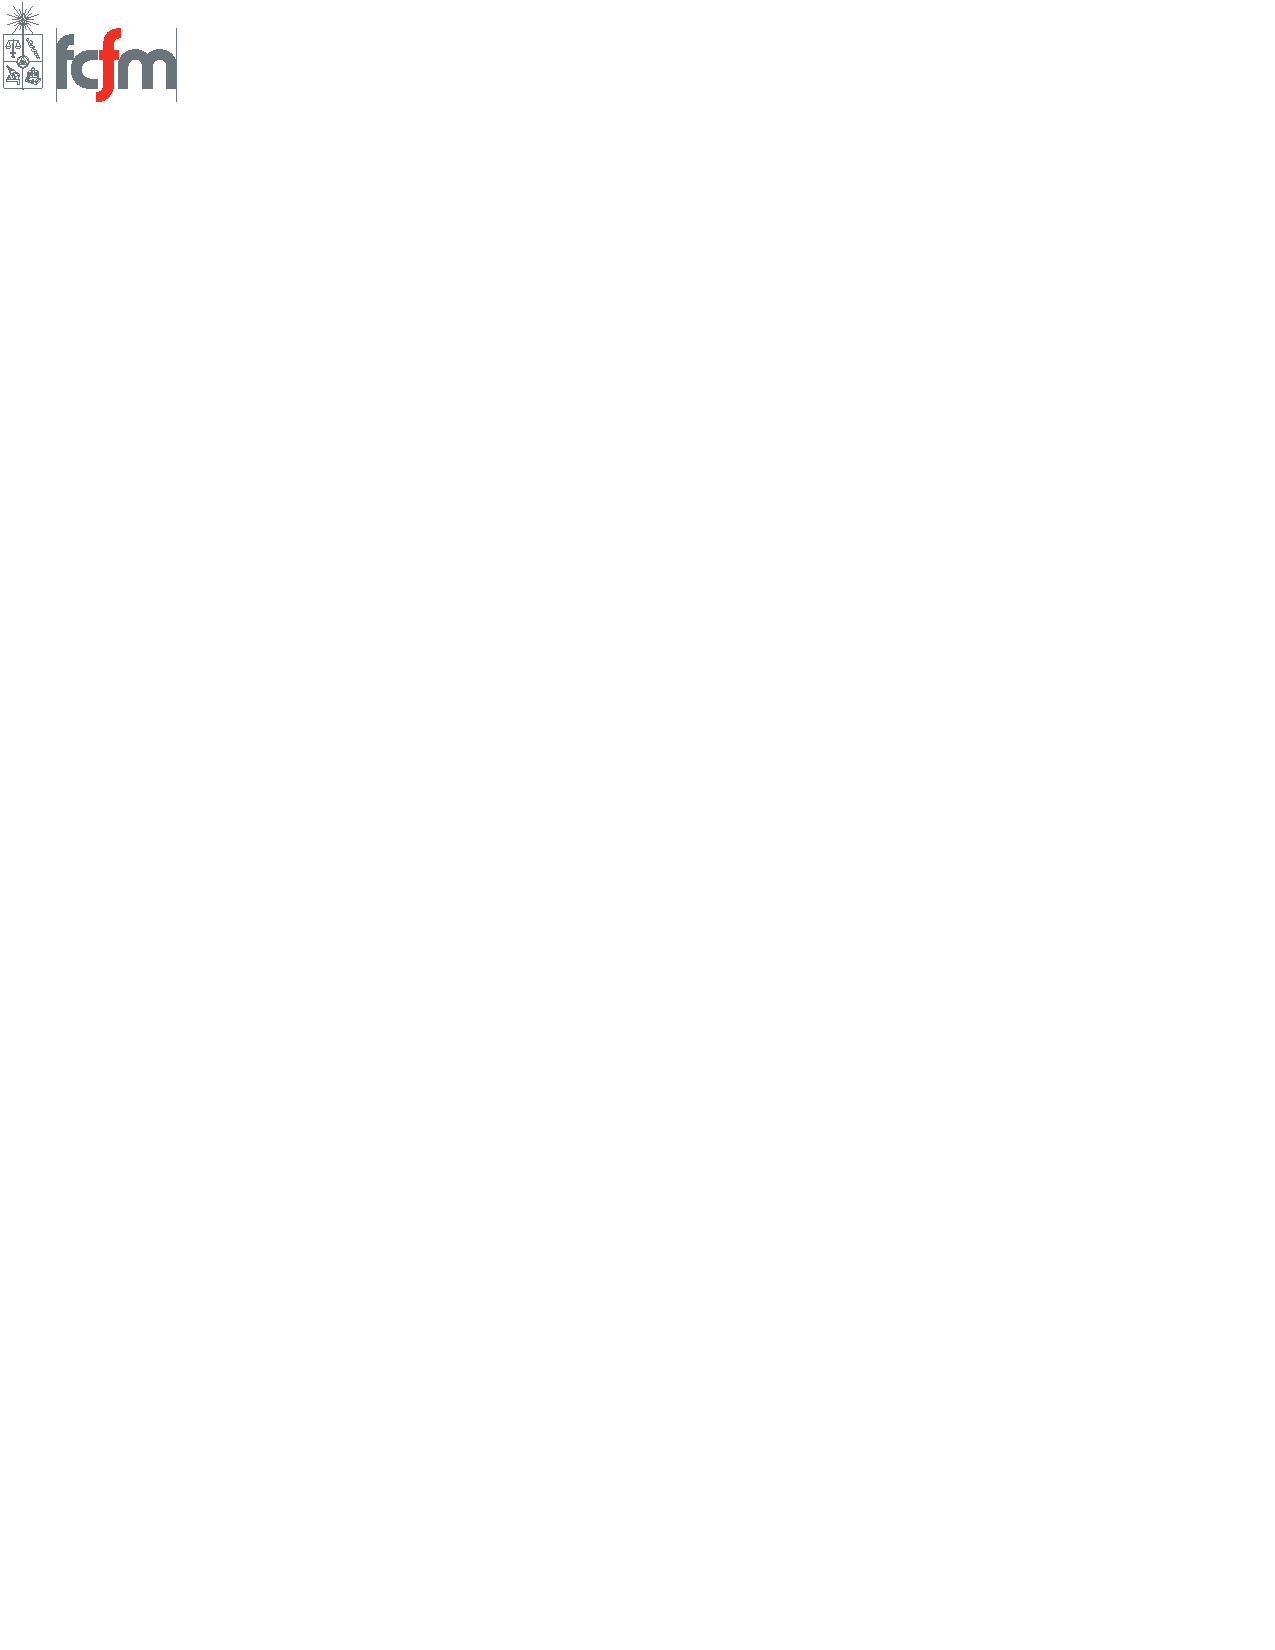
\includegraphics[scale=1.35]{fcfm2}
	\end{wrapfigure}
	\hspace*{0.05cm}
	\noindent \textsc{\color{red} \hspace{-2.2cm} \departamentouniversidad} ~ \\
	\hspace*{0.05cm}
	\noindent \textsc{\color{dkgray} \hspace{-1.6cm} \nombrefacultad} ~ \\
	\hspace*{0.05cm}
	\noindent \textsc{\color{dkgray} \hspace{-1.6cm} \nombreuniversidad} ~ \\
	\hspace*{0.05cm}
	\noindent \textsc{\color{dkgray} \hspace{-1.6cm} \codigodelcurso \nombredelcurso} ~ \\
	\vfill
	\begin{center}
		\vspace*{0.5cm}
		{\color{dkgray} \Large \textbf{\MakeUppercase{\temaatratar}}} ~ \\
		\noindent \rule{\linewidth}{0.3mm} ~ \\
		\Huge \textup \bfseries \textsc{\textcolor{\portraittitlecolor}{\titulodelinforme}} ~ \\
		\noindent \rule{\linewidth}{0.3mm} ~ \\
	\end{center}
	\begin{minipage}{.5\textwidth}
		~
	\end{minipage}
	\vfill
	\begin{minipage}{1.0\textwidth}
		\begin{flushright}
			\noindent \tablaintegrantes
		\end{flushright}
	\end{minipage}
}{
\ifthenelse{\equal{\portraitstyle}{style7}}{
	\setpagemargincm{\pagemarginleft}{\pagemargintop}{\pagemarginright}{\pagemarginbottom}
	\thispagestyle{empty}
	\begin{center}
		\vspace*{-1.5cm}
		\includegraphics[scale=\imagendepartamentoescala]{\imagendepartamento}
		\hspace*{-0.15cm}
		\begin{tabular}{l}
			\vspace*{0.26cm}\mbox{} ~ \\
			\small \textsc{\MakeUppercase{\nombreuniversidad}} ~ \\
			\small \textsc{\MakeUppercase{\nombrefacultad}} ~ \\
			\small \textsc{\MakeUppercase{\departamentouniversidad}} ~ \\
			\vspace*{1.25cm}\mbox{}
		\end{tabular}
	\end{center}
	\vfill
	\begin{center}
		\noindent \rule{\textwidth}{0.4mm} \\ \vspace{0.3cm}
		{\huge \textcolor{\portraittitlecolor}{\titulodelinforme} \vspace{0.2cm} ~ \\}
		\noindent \rule{\textwidth}{0.4mm} ~ \\ \vspace{0.40cm}
		{\large \textcolor{\portraittitlecolor}{\temaatratar} ~ \\}
	\end{center}
	\vfill
	\noindent
	\begin{minipage}{1.0\textwidth}
		\begin{flushright}
			\scshape{\tablaintegrantes}
		\end{flushright}
	\end{minipage}
}{
\ifthenelse{\equal{\portraitstyle}{style8}}{
	\setpagemargincm{\pagemarginleft}{\pagemargintop}{\pagemarginright}{\pagemarginbottom}
	\thispagestyle{empty}
	\begin{center}
		\vspace*{-1.0cm}
		\begin{tabular}{c}
			\includegraphics[scale=\imagendepartamentoescala]{\imagendepartamento} \vspace{0.5cm} ~ \\
			\small \scshape{\MakeUppercase{\nombreuniversidad}} ~ \\
			\small \scshape{\MakeUppercase{\nombrefacultad}} ~ \\
			\small \scshape{\MakeUppercase{\departamentouniversidad}}
		\end{tabular}
	\end{center}
	\vfill
	\begin{center}
		\noindent \rule{\textwidth}{0.4mm} \\ \vspace{0.3cm}
		{\huge \textcolor{\portraittitlecolor}{\titulodelinforme} \vspace{0.2cm} ~ \\}
		\noindent \rule{\textwidth}{0.4mm} ~ \\ \vspace{0.40cm}
		{\large \textcolor{\portraittitlecolor}{\temaatratar} ~ \\}
	\end{center}
	\vfill
	\noindent
	\begin{minipage}{1.0\textwidth}
		\begin{flushright}
			\scshape{\tablaintegrantes}
		\end{flushright}
	\end{minipage}
}{
\ifthenelse{\equal{\portraitstyle}{style9}}{
	\setpagemargincm{\pagemarginleft}{\pagemargintop}{\pagemarginright}{\pagemarginbottom}
	\thispagestyle{empty}
	\noindent \includegraphics[scale=\imagendepartamentoescala]{\imagendepartamento}
	\vfill
	\begin{center}
		\noindent \rule{\textwidth}{0.4mm} \\ \vspace{0.3cm}
		{\huge \textcolor{\portraittitlecolor}{\titulodelinforme} \vspace{0.2cm} \\}
		\noindent \rule{\textwidth}{0.4mm} \\ \vspace{0.35cm}
		{\large \textcolor{\portraittitlecolor}{\temaatratar} \\}
	\end{center}
	\vfill
	\begin{center}
		\begin{tabular}{c}
			\small \scshape{\MakeUppercase{\nombreuniversidad}} ~ \\
			\small \scshape{\MakeUppercase{\nombrefacultad}} ~ \\
			\small \scshape{\MakeUppercase{\departamentouniversidad}}
		\end{tabular}
	\end{center}
	\vfill
	\begin{center}
		\indent \scshape{\tablaintegrantes}
	\end{center}
}{
\ifthenelse{\equal{\portraitstyle}{style10}}{
	\setpagemargincm{\pagemarginleft}{\pagemargintop}{\pagemarginright}{\pagemarginbottom}
	\thispagestyle{empty}
	~ \\
	\vfill
	\begin{center}
		\ifthenelse{\equal{\nombreuniversidad}{\xspace}}{
			\noindent {\large \textsc{\departamentouniversidad}}
		}{
			\noindent {\large \textsc{\nombreuniversidad, \departamentouniversidad}}
		}
		\vspace{1.0cm}
	\end{center}
	\vfill
	\begin{center}
		\noindent {\large \scshape{\nombredelcurso}} \vspace{0.5cm} ~ \\
		\noindent {\large \scshape{\codigodelcurso}} \vspace{0.5cm} ~ \\
		\noindent \rule{\textwidth}{0.4mm} \\ \vspace{0.3cm}
		{\huge \bfseries \textcolor{\portraittitlecolor}{\titulodelinforme} \vspace{0.2cm} \\}
		\noindent \rule{\textwidth}{0.4mm} \\ \vspace{2.5cm}
	\end{center}
	\vfill
	\begin{center}
		\indent \tablaintegrantes
	\end{center}
	\vfill
	~ \\
}{
\ifthenelse{\equal{\portraitstyle}{style11}}{
	\setpagemargincm{\pagemarginleft}{\pagemargintop}{\pagemarginright}{\pagemarginbottom}
	\thispagestyle{empty}
	\begin{center}
		\vspace*{-1.0cm}
		\scshape{\nombreuniversidad} ~ \\
		\scshape{\nombrefacultad} ~ \\
		\scshape{\departamentouniversidad}
	\end{center}
	\vfill
	\begin{center}
		{\setstretch{1.2} \fontsize{21pt}{22pt} \selectfont \textcolor{\portraittitlecolor}{\scshape{\titulodelinforme}} \vspace{0.5cm}} ~ \\
		{\fontsize{13pt}{10pt} \selectfont \textcolor{\portraittitlecolor}{\scshape{\temaatratar}}}
	\end{center}
	\vfill
	\begin{center}
		\indent \tablaintegrantes
	\end{center}
}{
\ifthenelse{\equal{\portraitstyle}{style12}}{
	\setpagemargincm{\pagemarginleft}{\pagemargintop}{\pagemarginright}{\pagemarginbottom}
	\thispagestyle{empty}
	\begin{center}
		\vspace*{-1.0cm}
		\includegraphics[scale=\imagendepartamentoescala]{\imagendepartamento}
	\end{center}
	\vfill
	\begin{center}
		{\bf \Huge \scshape{\textcolor{\portraittitlecolor}{\titulodelinforme}} \vspace{0.3cm}} \\
		{\bf \Large \textcolor{\portraittitlecolor}{\temaatratar}}
	\end{center}
	\vfill
	\begin{flushright}
		\noindent \tablaintegrantes
	\end{flushright}
	\vspace{0.5cm}
	\noindent \rule{\textwidth}{0.4mm}
	\begin{center}
		\ifthenelse{\equal{\nombreuniversidad}{\xspace}}{
			\scshape{\nombrefacultad} \\
		}{
			\scshape{\nombreuniversidad, \nombrefacultad} \\
		}
		\scshape{\departamentouniversidad}
	\end{center}
}{
\ifthenelse{\equal{\portraitstyle}{style13}}{
	\setpagemargincm{\pagemarginleft}{\pagemargintop}{\pagemarginright}{\pagemarginbottom}
	\thispagestyle{empty}
	\noindent
	\vspace*{-1.5cm}
	\begin{flushleft}
		\begin{minipage}{0.65\textwidth}
			\ifthenelse{\equal{\nombreuniversidad}{\xspace}}{
				{\fontsize{3.5mm}{0.5mm} \selectfont \noindent \textsf{\nombrefacultad}} ~ \\
			}{
				{\fontsize{3.5mm}{0.5mm} \selectfont \noindent \textsf{\nombreuniversidad, \nombrefacultad}} ~ \\
			}
			\noindent {\fontsize{3.0mm}{0.5mm} \selectfont \textsf{\departamentouniversidad} \vspace{-0.2cm}} ~ \\
			\noindent \textcolor{gray}{\rule{\textwidth}{0.3mm}}
		\end{minipage}
	\end{flushleft}
	\vspace*{-2.15cm}
	\begin{flushright}
		\begin{minipage}{0.3\textwidth}
			\noindent \includegraphics[width=1.0\textwidth]{\imagendepartamento}
		\end{minipage}
	\end{flushright}
	\vfill
	\begin{center}
		\begin{minipage}{0.9\textwidth}
			\begin{framed}
				\LARGE
				\vspace{1cm}
				\centering \textcolor{\portraittitlecolor}{\textbf{\titulodelinforme}}
				\vspace{1cm}
			\end{framed}
		\end{minipage}
	\end{center}
	\vfill
	\begin{flushright}
		\noindent \textsf{\tablaintegrantes}
	\end{flushright}
}{
\ifthenelse{\equal{\portraitstyle}{style14}}{
	\setpagemargincm{\pagemarginleft}{\pagemargintop}{\pagemarginright}{\pagemarginbottom}
	\thispagestyle{empty}
	\noindent
	\begin{flushleft}
		\vspace*{-1.0cm}
		\noindent \includegraphics[scale=\imagendepartamentoescala]{\imagendepartamento} \\
	\end{flushleft}
	\vfill
	{\bf \huge \noindent \textcolor{\portraittitlecolor}{\textsf{\MakeUppercase{\titulodelinforme}} \vspace*{0.05cm}}} \\
	{\bf \large \noindent \textcolor{\portraittitlecolor}{\textsf{\MakeUppercase{\temaatratar}}}} \\
	\vfill
	\begin{flushright}
		\noindent \textsf{\tablaintegrantes}
	\end{flushright}
}{
\ifthenelse{\equal{\portraitstyle}{style15}}{
	\setpagemargincm{\pagemarginleft}{\pagemargintop}{\pagemarginright}{\pagemarginbottom}
	\thispagestyle{empty}
	\checkextravarexist{\headerimageA}{Defina la imagen extra de la portada en el archivo lib/page/portrait-config.tex (VERSION NORMAL) o bien en el bloque PORTADA (VERSION COMPACTA)}
	\checkextravarexist{\headerimagescaleA}{Defina la escala de la imagen extra de la portada en el archivo lib/page/portrait-config.tex (VERSION NORMAL) o bien en el bloque PORTADA (VERSION COMPACTA)}
	\vspace*{-1.5cm}
	\noindent \begin{minipage}{0.8\textwidth}
		\noindent \begin{minipage}{0.22\textwidth}
			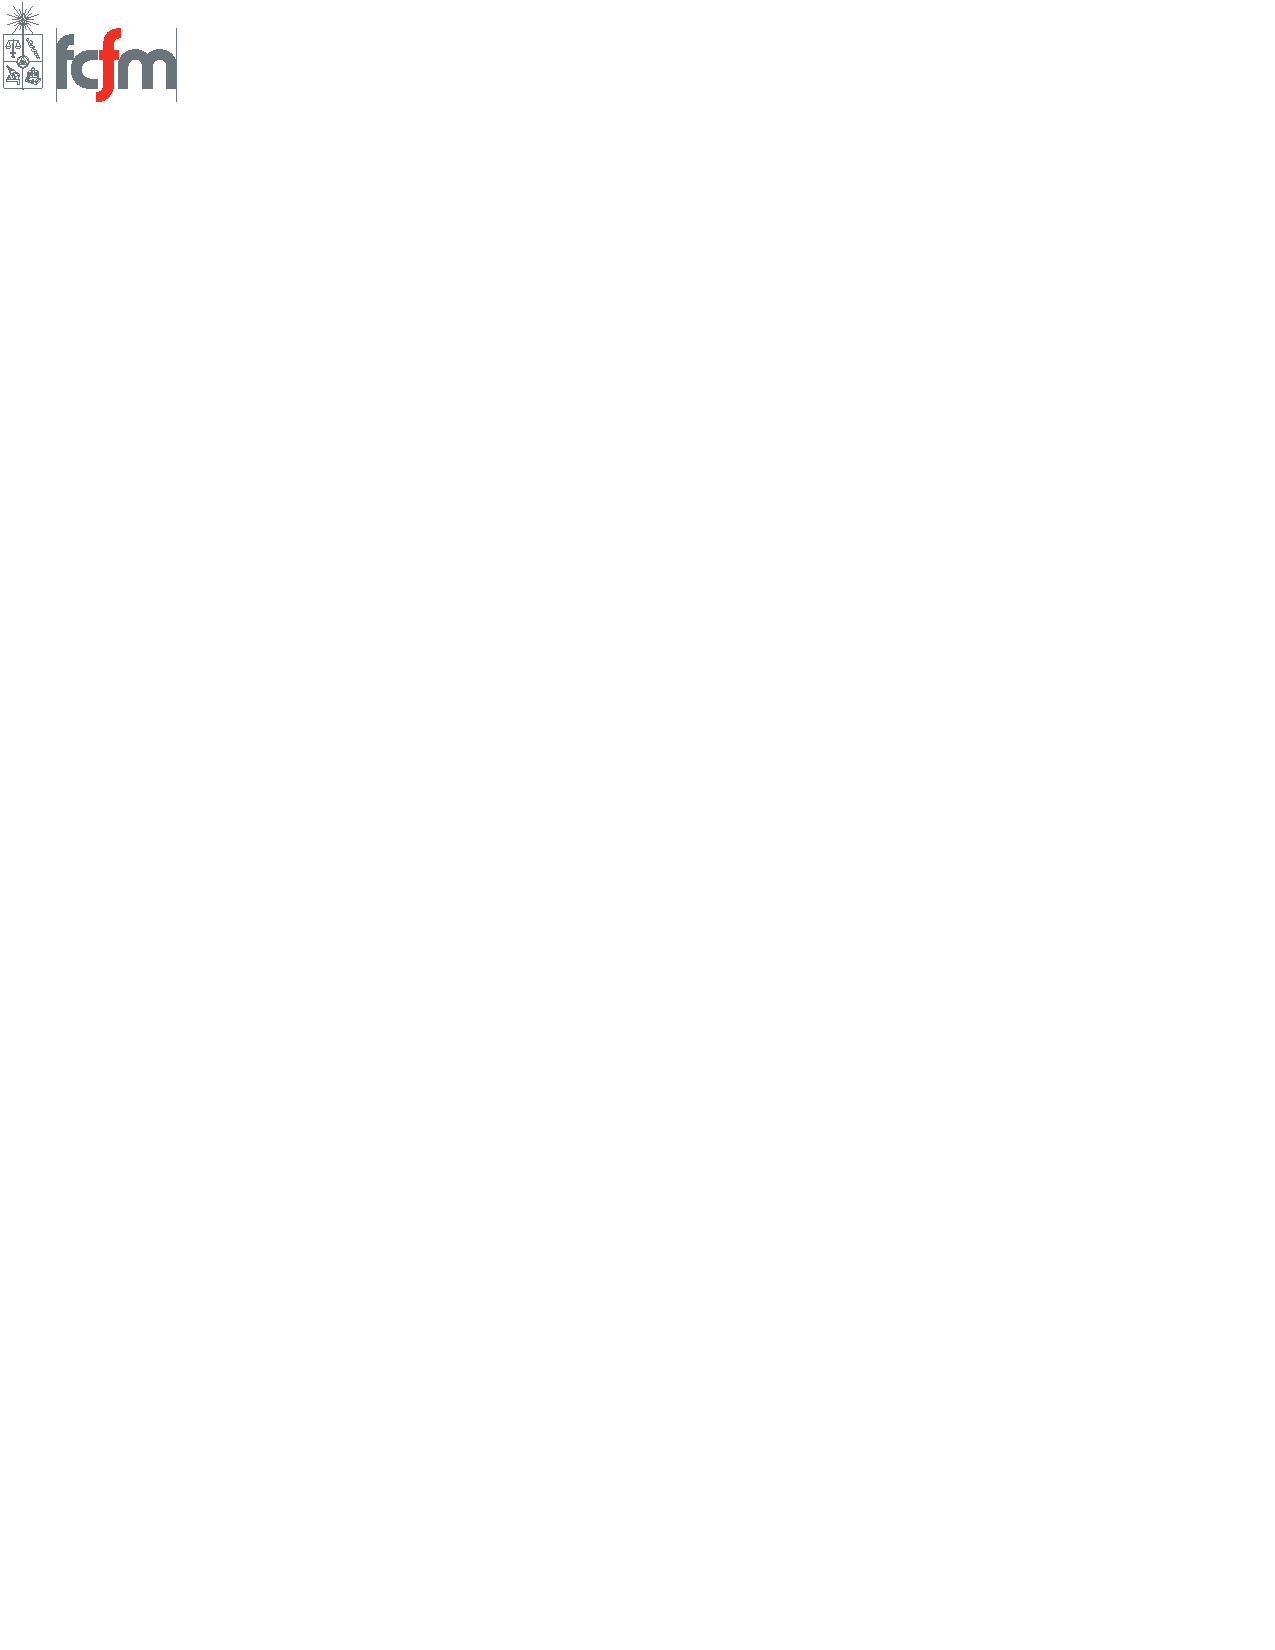
\includegraphics[scale=1.0]{fcfm2} \\
		\end{minipage}
		\begin{minipage}{0.6\textwidth}
			\begin{flushleft}
				\textsc{
				\begin{tabular}{l}
					{\small \nombreuniversidad} ~ \\
					{\small \nombrefacultad} ~ \\
					{\small \departamentouniversidad}
				\end{tabular}
				}
			\end{flushleft}
		\end{minipage}
	\end{minipage}
	\noindent \begin{minipage}{0.2\textwidth}
		\begin{flushright}
			\ifthenelse{\isundefined{\headerimageA}}{}{
				\ifthenelse{\isundefined{\headerimagescaleA}}{}{
					\noindent \includegraphics[scale=\headerimagescaleA]{\headerimageA} \\
				}
			}
		\end{flushright}
	\end{minipage}
	\vfill
	\begin{center}
		{\fontsize{25pt}{15pt} \selectfont \textcolor{\portraittitlecolor}{\textbf{\titulodelinforme}} \vspace{0.7cm}} \\
		{\Large \textcolor{\portraittitlecolor}{\temaatratar}}
	\end{center}
	\vfill
	\begin{center}
		\noindent \tablaintegrantes
	\end{center}
}{
\ifthenelse{\equal{\portraitstyle}{style16}}{
	\setpagemargincm{\pagemarginleft}{\pagemargintop}{\pagemarginright}{\pagemarginbottom}
	\checkextravarexist{\portraitbackgroundimageB}{[portrait-style16] Defina el fondo de la portada en el archivo lib/page/portrait-config.tex (VERSION NORMAL) o bien en el bloque PORTADA (VERSION COMPACTA)}
	\checkextravarexist{\portraitbackgroundcolorB}{[portrait-style16] Defina el color del bloque del titulo de la portada en el archivo lib/page/portrait-config.tex (VERSION NORMAL) o bien en el bloque PORTADA (VERSION COMPACTA)}
	\begingroup
		\thispagestyle{empty}
		\begin{tikzpicture}[remember picture,overlay]
			\node[inner sep=0pt] (background) at (current page.center) {\includegraphics[width=\paperwidth]{\portraitbackgroundimageB}};
			\draw (current page.center) node [fill=\portraitbackgroundcolorB!30!white,fill opacity=0.6,text opacity=1,inner sep=1cm]{\Huge\centering\bfseries\sffamily\parbox[c][][t]{\paperwidth}{
					\centering \textcolor{\portraittitlecolor}{\titulodelinforme} \\ [10pt]
					{\Large \textcolor{\portraittitlecolor}{\temaatratar}} \\ [25pt]
					{\huge \autordeldocumento}}};
		\end{tikzpicture}
		\vfill
	\endgroup
}{
\ifthenelse{\equal{\portraitstyle}{style17}}{
	\setpagemargincm{\pagemarginleft}{\firstpagemargintop}{\pagemarginright}{\pagemarginbottom}
	\pagestyle{fancy}
	\checkextravarexist{\portraitimageC}{[portrait-style17] Defina la imagen de la portada en el archivo lib/page/portrait-config.tex (VERSION NORMAL) o bien en el bloque PORTADA (VERSION COMPACTA)}
	\checkextravarexist{\portraitimageboxedC}{[portrait-style17] Defina si la imagen de la portada se encierra en un recuadro en el archivo lib/page/portrait-config.tex (VERSION NORMAL) o bien en el bloque PORTADA (VERSION COMPACTA)}
	\checkextravarexist{\portraitimageboxedwidthC}{[portrait-style17] Defina el grosor del recuadro de la imagen de la portada en el archivo lib/page/portrait-config.tex (VERSION NORMAL) o bien en el bloque PORTADA (VERSION COMPACTA)}
	\checkextravarexist{\portraitimagewidthC}{[portrait-style17] Defina los parametros de la imagen de la portada en el archivo lib/page/portrait-config.tex (VERSION NORMAL) o bien en el bloque PORTADA (VERSION COMPACTA)}
	\fancyhf{}
	\fancyhead[L]{
		\nombreuniversidad ~ \\
		\nombrefacultad ~ \\
		\departamentouniversidad ~ \\
		\vspace{-0.43cm}
	}
	\fancyhead[R]{
		\includegraphics[scale=\imagendepartamentoescala]{\imagendepartamento}
		\hspace{-0.255cm}
	}
	~ \\
	\vfill
	\begin{center}
		\textcolor{\portraittitlecolor}{
			{\noindent \Huge{\titulodelinforme} \vspace{0.5cm}} ~ \\
			{\noindent \large{\temaatratar}}
		}
	\end{center}
	~ \\
	\ifthenelse{\equal{\portraitimageboxedC}{true}}{
		\insertimageboxed{\portraitimageC}{width=\portraitimagewidthC}{\portraitimageboxedwidthC}{}
	}{
		\insertimage{\portraitimageC}{width=\portraitimagewidthC}{}
	}
	~ \\
	\vfill
	\noindent
	\begin{minipage}{1.0\textwidth}
		\begin{flushright}
			\tablaintegrantes
		\end{flushright}
	\end{minipage}
}{
\ifthenelse{\equal{\portraitstyle}{style18}}{
	\setpagemargincm{\pagemarginleft}{\firstpagemargintop}{\pagemarginright}{\pagemarginbottom}
	\pagestyle{fancy}
	\checkextravarexist{\portraitimageD}{[portrait-style18] Defina la imagen de la portada en el archivo lib/page/portrait-config.tex (VERSION NORMAL) o bien en el bloque PORTADA (VERSION COMPACTA)}
	\checkextravarexist{\portraitimageboxedD}{[portrait-style18] Defina si la imagen de la portada se encierra en un recuadro en el archivo lib/page/portrait-config.tex (VERSION NORMAL) o bien en el bloque PORTADA (VERSION COMPACTA)}
	\checkextravarexist{\portraitimageboxedwidthD}{[portrait-style18] Defina el grosor del recuadro de la imagen de la portada en el archivo lib/page/portrait-config.tex (VERSION NORMAL) o bien en el bloque PORTADA (VERSION COMPACTA)}
	\checkextravarexist{\portraitimagewidthD}{[portrait-style18] Defina los parametros de la imagen de la portada en el archivo lib/page/portrait-config.tex (VERSION NORMAL) o bien en el bloque PORTADA (VERSION COMPACTA)}
	\fancyhf{}
	\fancyhead[L]{
		\nombreuniversidad ~ \\
		\nombrefacultad ~ \\
		\departamentouniversidad ~ \\
		\vspace{-0.43cm}
	}
	\fancyhead[R]{
		\includegraphics[scale=\imagendepartamentoescala]{\imagendepartamento}
		\hspace{-0.255cm}
	}
	~ \\
	\ifthenelse{\equal{\portraitimageboxedD}{true}}{
		\insertimageboxed{\portraitimageD}{width=\portraitimagewidthD}{\portraitimageboxedwidthD}{}
	}{
		\insertimage{\portraitimageD}{width=\portraitimagewidthD}{}
	}
	\vfill
	\begin{center}
		\textcolor{\portraittitlecolor}{
			{\noindent \Huge{\titulodelinforme} \vspace{0.5cm}} ~ \\
			{\noindent \large{\temaatratar}}
		}
	\end{center}
	\vfill
	\noindent
	\begin{minipage}{1.0\textwidth}
		\begin{flushright}
			\tablaintegrantes
		\end{flushright}
	\end{minipage}
}{
\ifthenelse{\equal{\portraitstyle}{style19}}{
	\setpagemargincm{\pagemarginleft}{\pagemargintop}{\pagemarginright}{\pagemarginbottom}
	\thispagestyle{empty}
	\vspace*{0cm}
	\begin{center}
		\noindent \rule{\textwidth}{0.4mm} \\ \vspace{0.3cm}
		{\huge \bfseries \textcolor{\portraittitlecolor}{\titulodelinforme} \vspace{0.2cm} \\}
		\noindent \rule{\textwidth}{0.4mm}
	\end{center}
	~ \\
	\begin{center}
		\noindent {\large \scshape{\codigodelcurso} \large \scshape{\nombredelcurso}} \vspace{0.5cm} ~ \\
		\ifthenelse{\equal{\nombreuniversidad}{\xspace}}{
			\noindent {\large \textsc{\departamentouniversidad}}
		}{
			\noindent {\large \textsc{\nombreuniversidad, \departamentouniversidad}}
		}
		\vspace{1.0cm}
	\end{center}
	\vfill
	\begin{center}
		\indent \tablaintegrantes
	\end{center}
	~ \\
}{
\ifthenelse{\equal{\portraitstyle}{style20}}{
	\setpagemargincm{\pagemarginleft}{\pagemargintop}{\pagemarginright}{\pagemarginbottom}
	\thispagestyle{empty}
	{\raggedleft	
	\rule{1pt}{\textheight}
	\hspace{0.05\textwidth}
	\parbox[b]{0.75\textwidth}{
		{\Huge\bfseries \textcolor{\portraittitlecolor}{\titulodelinforme}}\\[2\baselineskip]
		{\large\textit{\textcolor{\portraittitlecolor}{\temaatratar}}}\\[4\baselineskip]
		\vspace*{2cm}
		{\textsc{
		\begin{flushleft}
			\noindent\tablaintegrantes
		\end{flushleft}
		}}
		\vspace*{\portraitverticalspaceE}
		{\noindent \nombreuniversidad ~\\
		\nombrefacultad ~\\
		\departamentouniversidad}\\[\baselineskip]
	}}
}{
\ifthenelse{\equal{\portraitstyle}{\bgtemplatetestcode}}{
	\setpagemargincm{\pagemarginleft}{\pagemargintop}{\pagemarginright}{\pagemarginbottom}
	\pagestyle{empty}
	\pagecolor{lbrown}
	\begin{center}
		\vspace*{-1.0cm}
		\scshape{\nombreuniversidad} ~ \\
		\scshape{\nombrefacultad} ~ \\
		\scshape{\departamentouniversidad}
	\end{center}
	~ \\
	\begin{center}
		\bgtemplatetestimg
	\end{center}
	\begin{center}
		\vspace*{-6cm}
		{\setstretch{1.2} \fontsize{25pt}{22pt} \selectfont \textcolor{\portraittitlecolor}{\scshape{\titulodelinforme}} \vspace{0.5cm}} \\
		{\fontsize{15pt}{10pt} \selectfont \textcolor{\portraittitlecolor}{\scshape{\temaatratar}}}
	\end{center}
	\vfill
	\begin{flushright}
		\noindent \tablaintegrantes
	\end{flushright}
	\newpage
	\pagecolor{\colorpage}
}{
	\throwbadconfigondoc{Estilo de portada incorrecto}{\portraitstyle}{style1 .. style20}}}}}}}}}}}}}}}}}}}}}
}
\ifthenelse{\equal{\addemptypagetwosides}{true}}{
	\newpage
	\null
	\thispagestyle{empty}
	\renewcommand{\thepage}{}
	\newpage}{
}
 % Se puede borrar

% CONFIGURACIÓN DE PÁGINA Y ENCABEZADOS
% Template:     Informe/Reporte LaTeX
% Documento:    Configuración de página
% Versión:      6.4.4 (13/08/2019)
% Codificación: UTF-8
%
% Autor: Pablo Pizarro R. @ppizarror
%        Facultad de Ciencias Físicas y Matemáticas
%        Universidad de Chile
%        pablo.pizarro@ing.uchile.cl, ppizarror.com
%
% Manual template: [https://latex.ppizarror.com/Template-Informe/]
% Licencia MIT:    [https://opensource.org/licenses/MIT/]

\newpage
\ifthenelse{\equal{\predocpageromannumber}{true}}{
	\ifthenelse{\equal{\predocpageromanupper}{true}}{
		\pagenumbering{Roman}
	}{
		\pagenumbering{roman}
	}}{
	\pagenumbering{arabic}
}
\setcounter{page}{1}
\setcounter{footnote}{0}
\setpagemargincm{\pagemarginleft}{\pagemargintop}{\pagemarginright}{\pagemarginbottom}
\def\arraystretch {\tablepaddingv}
\setlength{\tabcolsep}{\tablepaddingh em}
\ifthenelse{\equal{\pointdecimal}{true}}{
	\decimalpoint}{
}
\renewcommand{\appendixname}{\nomltappendixsection}
\renewcommand{\appendixpagename}{\nameappendixsection}
\renewcommand{\appendixtocname}{\nameappendixsection}
\renewcommand{\contentsname}{\nomltcont}
\renewcommand{\figurename}{\nomltwfigure}
\renewcommand{\listfigurename}{\nomltfigure}
\renewcommand{\listtablename}{\nomlttable}
\renewcommand{\lstlistingname}{\nomltwsrc}
\renewcommand{\lstlistlistingname}{\nomltsrc}
\renewcommand{\refname}{\namereferences}
\renewcommand{\tablename}{\nomltwtable}
\sectionfont{\color{\titlecolor} \fontsizetitle \styletitle \selectfont}
\subsectionfont{\color{\subtitlecolor} \fontsizesubtitle \stylesubtitle \selectfont}
\subsubsectionfont{\color{\subsubtitlecolor} \fontsizesubsubtitle \stylesubsubtitle \selectfont}
\titleformat{\subsubsubsection}{\color{\ssstitlecolor} \normalfont \fontsizessstitle \stylessstitle}{\thesubsubsubsection}{1em}{}
\titlespacing*{\subsubsubsection}{0pt}{3.25ex plus 1ex minus .2ex}{1.5ex plus .2ex}
\ifthenelse{\equal{\hfstyle}{style1}}{
	\pagestyle{fancy} \fancyhf{}
	\ifthenelse{\equal{\disablehfrightmark}{false}}{
		\fancyhead[L]{\nouppercase{\rightmark}}
	}{}
	\fancyhead[R]{\small \thepage}
	\ifthenelse{\equal{\hfwidthwrap}{true}}{
		\fancyfoot[L]{
			\begin{minipage}[t]{\hfwidthtitle\linewidth}
				\begin{flushleft}
					\small \textit{\titulodelinforme}
				\end{flushleft}
			\end{minipage}
		}
		\fancyfoot[R]{
			\begin{minipage}[t]{\hfwidthcourse\linewidth}
				\begin{flushright}
					\small \textit{\codigodelcurso \nombredelcurso}
				\end{flushright}
			\end{minipage}
		}
	}{
		\fancyfoot[L]{\small \textit{\titulodelinforme}}
		\fancyfoot[R]{\small \textit{\codigodelcurso \nombredelcurso}}
	}
	\renewcommand{\headrulewidth}{0.5pt}
	\renewcommand{\footrulewidth}{0.5pt}
	\renewcommand{\sectionmark}[1]{\markboth{#1}{}}
}{
\ifthenelse{\equal{\hfstyle}{style2}}{
	\pagestyle{fancy} \fancyhf{}
	\ifthenelse{\equal{\disablehfrightmark}{false}}{
		\fancyhead[L]{\nouppercase{\rightmark}}
	}{}
	\fancyhead[R]{\small \thepage}
	\ifthenelse{\equal{\hfwidthwrap}{true}}{
		\fancyfoot[L]{
			\begin{minipage}[t]{\hfwidthtitle\linewidth}
				\begin{flushleft}
					\small \textit{\titulodelinforme}
				\end{flushleft}
			\end{minipage}
		}
		\fancyfoot[R]{
			\begin{minipage}[t]{\hfwidthcourse\linewidth}
				\begin{flushright}
					\small \textit{\codigodelcurso \nombredelcurso}
				\end{flushright}
			\end{minipage}
		}
	}{
		\fancyfoot[L]{\small \textit{\titulodelinforme}}
		\fancyfoot[R]{\small \textit{\codigodelcurso \nombredelcurso}}
	}
	\renewcommand{\headrulewidth}{0.5pt}
	\renewcommand{\footrulewidth}{0pt}
	\renewcommand{\sectionmark}[1]{\markboth{#1}{}}
}{
\ifthenelse{\equal{\hfstyle}{style3}}{
	\pagestyle{fancy} \fancyhf{}
	\ifthenelse{\equal{\hfwidthwrap}{true}}{
		\fancyhead[L]{
			\begin{minipage}[t]{\hfwidthtitle\linewidth}
				\begin{flushleft}
					\small \textit{\codigodelcurso \nombredelcurso}
				\end{flushleft}
			\end{minipage}
		}
	}{
		\fancyhead[L]{\small \textit{\codigodelcurso \nombredelcurso}}
	}
	\fancyhead[R]{
		\includegraphics[width=1.2cm]{\imagendepartamento}
		\vspace{-0.15cm}
	}
	\fancyfoot[C]{\thepage}
	\renewcommand{\headrulewidth}{0.5pt}
	\renewcommand{\footrulewidth}{0pt}
}{
\ifthenelse{\equal{\hfstyle}{style4}}{
	\pagestyle{fancy} \fancyhf{}
	\ifthenelse{\equal{\disablehfrightmark}{false}}{
		\fancyhead[L]{\nouppercase{\rightmark}}
	}{}
	\fancyhead[R]{}
	\fancyfoot[C]{\small \thepage}
	\renewcommand{\headrulewidth}{0.5pt}
	\renewcommand{\footrulewidth}{0pt}
	\renewcommand{\sectionmark}[1]{\markboth{#1}{}}
}{
\ifthenelse{\equal{\hfstyle}{style5}}{
	\pagestyle{fancy} \fancyhf{}
	\ifthenelse{\equal{\hfwidthwrap}{true}}{
		\fancyhead[L]{
			\begin{minipage}[t]{\hfwidthcourse\linewidth}
				\begin{flushleft}
					\codigodelcurso \nombredelcurso
				\end{flushleft}
			\end{minipage}
		}
		\ifthenelse{\equal{\disablehfrightmark}{false}}{
			\fancyhead[R]{
				\begin{minipage}[t]{\hfwidthtitle\linewidth}
					\begin{flushright}
						\nouppercase{\rightmark}
					\end{flushright}
				\end{minipage}
			}
		}{}
	}{
		\fancyhead[L]{\codigodelcurso \nombredelcurso}
		\ifthenelse{\equal{\disablehfrightmark}{false}}{
			\fancyhead[R]{\nouppercase{\rightmark}}
		}{}
	}
	\fancyfoot[L]{\departamentouniversidad, \nombreuniversidad}
	\fancyfoot[R]{\small \thepage}
	\renewcommand{\headrulewidth}{0pt}
	\renewcommand{\footrulewidth}{0pt}
	\renewcommand{\sectionmark}[1]{\markboth{#1}{}}
}{
\ifthenelse{\equal{\hfstyle}{style6}}{
	\pagestyle{fancy} \fancyhf{}
	\fancyfoot[L]{\departamentouniversidad}
	\fancyfoot[C]{\thepage}
	\fancyfoot[R]{\nombreuniversidad}
	\renewcommand{\headrulewidth}{0pt}
	\renewcommand{\footrulewidth}{0pt}
	\setlength{\headheight}{49pt}
}{
\ifthenelse{\equal{\hfstyle}{style7}}{
	\pagestyle{fancy} \fancyhf{}
	\fancyfoot[C]{\thepage}
	\renewcommand{\headrulewidth}{0pt}
	\renewcommand{\footrulewidth}{0pt}
	\setlength{\headheight}{49pt}
}{
\ifthenelse{\equal{\hfstyle}{style8}}{
	\pagestyle{fancy} \fancyhf{}
	\fancyfoot[R]{\thepage}
	\renewcommand{\headrulewidth}{0pt}
	\renewcommand{\footrulewidth}{0pt}
	\setlength{\headheight}{49pt}
}{
\ifthenelse{\equal{\hfstyle}{style9}}{
	\pagestyle{fancy} \fancyhf{}
	\ifthenelse{\equal{\disablehfrightmark}{false}}{
		\fancyhead[L]{\nouppercase{\rightmark}}
	}{}
	\fancyhead[R]{}
	\fancyfoot[L]{\small \textit{\titulodelinforme}}
	\fancyfoot[R]{\small \thepage}
	\renewcommand{\headrulewidth}{0.5pt}
	\renewcommand{\footrulewidth}{0.5pt}
	\renewcommand{\sectionmark}[1]{\markboth{#1}{}}
}{
\ifthenelse{\equal{\hfstyle}{style10}}{
	\pagestyle{fancy} \fancyhf{}
	\ifthenelse{\equal{\hfwidthwrap}{true}}{
		\ifthenelse{\equal{\disablehfrightmark}{false}}{
			\fancyhead[L]{
				\begin{minipage}[t]{\hfwidthtitle\linewidth}
					\begin{flushleft}
						\nouppercase{\rightmark}
					\end{flushleft}
				\end{minipage}
			}
		}{}
		\fancyhead[R]{
			\begin{minipage}[t]{\hfwidthcourse\linewidth}
				\begin{flushright}
					\small \textit{\titulodelinforme}
				\end{flushright}
			\end{minipage}
		}
	}{
		\ifthenelse{\equal{\disablehfrightmark}{false}}{
			\fancyhead[L]{\nouppercase{\rightmark}}
		}{}
		\fancyhead[R]{\small \textit{\titulodelinforme}}
	}
	\fancyfoot[L]{}
	\fancyfoot[R]{\small \thepage}
	\renewcommand{\headrulewidth}{0.5pt}
	\renewcommand{\footrulewidth}{0.5pt}
	\renewcommand{\sectionmark}[1]{\markboth{#1}{}}
}{
\ifthenelse{\equal{\hfstyle}{style11}}{
	\pagestyle{fancy} \fancyhf{}
	\ifthenelse{\equal{\disablehfrightmark}{false}}{
		\fancyhead[L]{\nouppercase{\rightmark}}
	}{}
	\fancyhead[R]{\small \thepage \nomnpageof \pageref{LastPage}}
	\ifthenelse{\equal{\hfwidthwrap}{true}}{
		\fancyfoot[L]{
			\begin{minipage}[t]{\hfwidthtitle\linewidth}
				\begin{flushleft}
					\small \textit{\titulodelinforme}
				\end{flushleft}
			\end{minipage}
		}
		\fancyfoot[R]{
			\begin{minipage}[t]{\hfwidthcourse\linewidth}
				\begin{flushright}
					\small \textit{\codigodelcurso \nombredelcurso}
				\end{flushright}
			\end{minipage}
		}
	}{
		\fancyfoot[L]{\small \textit{\titulodelinforme}}
		\fancyfoot[R]{\small \textit{\codigodelcurso \nombredelcurso}}
	}
	\renewcommand{\headrulewidth}{0.5pt}
	\renewcommand{\footrulewidth}{0.5pt}
	\renewcommand{\sectionmark}[1]{\markboth{#1}{}}
}{
\ifthenelse{\equal{\hfstyle}{style12}}{
	\pagestyle{fancy} \fancyhf{}
	\fancyfoot[L]{\departamentouniversidad}
	\fancyfoot[C]{\thepage \nomnpageof \pageref{LastPage}}
	\fancyfoot[R]{\nombreuniversidad}
	\renewcommand{\headrulewidth}{0pt}
	\renewcommand{\footrulewidth}{0pt}
	\setlength{\headheight}{49pt}
}{
\ifthenelse{\equal{\hfstyle}{style13}}{
	\pagestyle{fancy} \fancyhf{}
	\ifthenelse{\equal{\hfwidthwrap}{true}}{
		\fancyhead[L]{
			\begin{minipage}[t]{\hfwidthtitle\linewidth}
				\begin{flushleft}
					\small \textit{\codigodelcurso \nombredelcurso}
				\end{flushleft}
			\end{minipage}
		}
	}{
		\fancyhead[L]{\small \textit{\codigodelcurso \nombredelcurso}}
	}
	\fancyhead[R]{
		\includegraphics[width=1.2cm]{\imagendepartamento}
		\vspace{-0.15cm}
	}
	\fancyfoot[C]{\thepage \nomnpageof \pageref{LastPage}}
	\renewcommand{\headrulewidth}{0.5pt}
	\renewcommand{\footrulewidth}{0pt}
}{
\ifthenelse{\equal{\hfstyle}{style14}}{
	\pagestyle{fancy} \fancyhf{}
	\ifthenelse{\equal{\disablehfrightmark}{false}}{
		\fancyhead[L]{\nouppercase{\rightmark}}
	}{}
	\fancyhead[R]{}
	\fancyfoot[C]{\small \thepage \nomnpageof \pageref{LastPage}}
	\renewcommand{\headrulewidth}{0.5pt}
	\renewcommand{\footrulewidth}{0pt}
	\renewcommand{\sectionmark}[1]{\markboth{#1}{}}
}{
\ifthenelse{\equal{\hfstyle}{style15}}{
	\pagestyle{fancy} \fancyhf{}
	\ifthenelse{\equal{\disablehfrightmark}{false}}{
		\fancyhead[L]{\nouppercase{\rightmark}}
	}{}
	\fancyhead[R]{}
	\fancyfoot[L]{
		\small \codigodelcurso \nombredelcurso
	}
	\fancyfoot[R]{
		\small \thepage
	}
	\renewcommand{\headrulewidth}{0.5pt}
	\renewcommand{\footrulewidth}{0.5pt}
	\renewcommand{\sectionmark}[1]{\markboth{#1}{}}
}{
\ifthenelse{\equal{\hfstyle}{style16}}{
	\pagestyle{fancy} \fancyhf{}
	\renewcommand{\headrulewidth}{0pt}
	\renewcommand{\footrulewidth}{0pt}
	\renewcommand{\sectionmark}[1]{\markboth{#1}{}}
}{
	\throwbadconfigondoc{Estilo de header-footer incorrecto}{\hfstyle}{style1 .. style16}}}}}}}}}}}}}}}}
}
\ifthenelse{\equal{\showlinenumbers}{true}}{
	\linenumbers}{
}


% RESUMEN O ABSTRACT
\begin{resumen}
%	\lipsum[1] % Párrafo ejemplo, se puede borrar
En esta tarea se estudia el uso de un controlador directo adaptativo a una planta inestable en función de un modelo de referencia. Por ello, se hace indispensable mostrar el desarrollo de las leyes de ajuste y comprender su significado e impacto en el sistema con el fin tener una intuición de la respuesta del sistema ante un valor externo. Un ejemplo de esto se puede ver cuando se cambian las condiciones iniciales de la planta mostrando que para algunos valores el error puede crecer grandemente en ordenes de magnitud. Si por lo demás se encuentra un perturbación en la salida de la plata no conocida, el error no será acotado y los parámetros de las leyes de ajuste dejan de converger.  \\
Para solucionar este método se trabaja con 4 métodos que modifican las leyes de ajuste en función de crear un controlador robusto e base a la perturbación entrante al sistema. \\
Finalmente, se ve el caso cuando la planta del sistema tiene un termino variable en el tiempo y se acotan os parámetros del error de la planta y de los parámetros con métodos de control robusto.
\end{resumen}

% TABLA DE CONTENIDOS - ÍNDICE
% Template:     Informe/Reporte LaTeX
% Documento:    Índice
% Versión:      6.4.4 (13/08/2019)
% Codificación: UTF-8
%
% Autor: Pablo Pizarro R. @ppizarror
%        Facultad de Ciencias Físicas y Matemáticas
%        Universidad de Chile
%        pablo.pizarro@ing.uchile.cl, ppizarror.com
%
% Manual template: [https://latex.ppizarror.com/Template-Informe/]
% Licencia MIT:    [https://opensource.org/licenses/MIT/]

\ifthenelse{\equal{\showindex}{true}}{
	\newpage
	\begingroup
	\sectionfont{\color{\indextitlecolor} \fontsizetitlei \styletitlei \selectfont}
	\ifthenelse{\equal{\addemptypagetwosides}{true}}{
		\checkoddpage
		\ifoddpage
		\else
			\newpage
			\null
			\thispagestyle{empty}
			\newpage
			\addtocounter{page}{-1}
		\fi}{
	}
	\ifthenelse{\equal{\addindextobookmarks}{true}}{
		\belowpdfbookmark{\nomltcont}{contents}}{
	}
	\tocloftpagestyle{fancy}
	\ifthenelse{\equal{\showdotaftersnum}{true}}{		
		\def\cftsecaftersnum {.}
		\def\cftsubsecaftersnum {.}
		\def\cftsubsubsecaftersnum {.}
		\def\cftsubsubsubsecaftersnum {.}
		\def\cftsecnumwidth {1.9em}
\def\cftsubsecnumwidth {2.57em}
\renewcommand\cftsubsubsecnumwidth{3.35em}
		\setlength{\cftsubsecindent}{1.91em}
\setlength{\cftsubsubsecindent}{4.48em}
		}{
	}
	\renewcommand{\cftdot}{\charnumpageindex}
	\def\cftfigaftersnum {\charafterobjectindex\enspace}
	\def\cftsubfigaftersnum {\charafterobjectindex\enspace}
	\def\cfttabaftersnum {\charafterobjectindex\enspace}
	\def\cftlstlistingaftersnum {\charafterobjectindex\enspace}
	\ifthenelse{\equal{\showlinenumbers}{true}}{
		\nolinenumbers}{
	}
	\ifthenelse{\equal{\objectindexindent}{true}}{
		\setlength{\cfttabindent}{1.9em}
		\setlength{\cftfigindent}{1.9em}
		\setlength{\cftsubfigindent}{1.9em}
		\setlength{\cftfigindent}{1.9em}
		\def\cftlstlistingindent {1.9em}
	}{
		\setlength{\cfttabindent}{0em}
		\setlength{\cftfigindent}{0em}
		\setlength{\cftsubfigindent}{0em}
		\setlength{\cftfigindent}{0em}
		\def\cftlstlistingindent {0em}
	}
	\ifthenelse{\equal{\showsectioncaptioncode}{none}}{
\def\cftdefautnumwidthcode {3.0em}
\def\cftdefaultnumwidthromancode {5.25em}
	}{
	\ifthenelse{\equal{\showsectioncaptioncode}{sec}}{
		\def\cftdefautnumwidthcode {3.7em}
		\def\cftdefaultnumwidthromancode {5.75em}
	}{
	\ifthenelse{\equal{\showsectioncaptioncode}{ssec}}{
		\def\cftdefautnumwidthcode {4.4em}
		\def\cftdefaultnumwidthromancode {6.25em}
	}{
	\ifthenelse{\equal{\showsectioncaptioncode}{sssec}}{
		\def\cftdefautnumwidthcode {5.1em}
		\def\cftdefaultnumwidthromancode {6.75em}
	}{
	\ifthenelse{\equal{\showsectioncaptioncode}{ssssec}}{
		\def\cftdefautnumwidthcode {5.8em}
		\def\cftdefaultnumwidthromancode {7.25em}
	}{
		\throwbadconfig{Valor configuracion incorrecto}{\showsectioncaptioncode}{none,sec,ssec,sssec,ssssec}}}}}
	}
	\ifthenelse{\equal{\showsectioncaptionfig}{none}}{
\def\cftdefautnumwidthfig {3.0em}
\def\cftdefaultnumwidthromanfig {5.25em}
	}{
	\ifthenelse{\equal{\showsectioncaptionfig}{sec}}{
		\def\cftdefautnumwidthfig {3.7em}
		\def\cftdefaultnumwidthromanfig {5.75em}
	}{
	\ifthenelse{\equal{\showsectioncaptionfig}{ssec}}{
		\def\cftdefautnumwidthfig {4.4em}
		\def\cftdefaultnumwidthromanfig {6.25em}
	}{
	\ifthenelse{\equal{\showsectioncaptionfig}{sssec}}{
		\def\cftdefautnumwidthfig {5.1em}
		\def\cftdefaultnumwidthromanfig {6.75em}
	}{
	\ifthenelse{\equal{\showsectioncaptionfig}{ssssec}}{
		\def\cftdefautnumwidthfig {5.8em}
		\def\cftdefaultnumwidthromanfig {7.25em}
	}{
		\throwbadconfig{Valor configuracion incorrecto}{\showsectioncaptionfig}{none,sec,ssec,sssec,ssssec}}}}}
	}
	\ifthenelse{\equal{\showsectioncaptiontab}{none}}{
\def\cftdefautnumwidthtab {3.0em}
\def\cftdefaultnumwidthromantab {5.25em}
	}{
	\ifthenelse{\equal{\showsectioncaptiontab}{sec}}{
		\def\cftdefautnumwidthtab {3.7em}
		\def\cftdefaultnumwidthromantab {5.75em}
	}{
	\ifthenelse{\equal{\showsectioncaptiontab}{ssec}}{
		\def\cftdefautnumwidthtab {4.4em}
		\def\cftdefaultnumwidthromantab {6.25em}
	}{
	\ifthenelse{\equal{\showsectioncaptiontab}{sssec}}{
		\def\cftdefautnumwidthtab {5.1em}
		\def\cftdefaultnumwidthromantab {6.75em}
	}{
	\ifthenelse{\equal{\showsectioncaptiontab}{ssssec}}{
		\def\cftdefautnumwidthtab {5.8em}
		\def\cftdefaultnumwidthromantab {7.25em}
	}{
		\throwbadconfig{Valor configuracion incorrecto}{\showsectioncaptiontab}{none,sec,ssec,sssec,ssssec}}}}}
	}
	\def\cftfignumwidth {\cftdefautnumwidth}
	\def\cfttabnumwidth {\cftdefautnumwidth}
	\def\cftlstlistingnumwidth {\cftdefautnumwidth}
\ifthenelse{\equal{\captionnumcode}{arabic}}{
		\def\cftlstlistingnumwidth {\cftdefautnumwidthcode}
	}{
		\ifthenelse{\equal{\captionnumcode}{roman}}{
			\def\cftlstlistingnumwidth {\cftdefaultnumwidthromancode}
		}{
		\ifthenelse{\equal{\captionnumcode}{Roman}}{
			\def\cftlstlistingnumwidth {\cftdefaultnumwidthromancode}
		}{
			\def\cftlstlistingnumwidth {\cftdefautnumwidthcode}
		}}
	}
\ifthenelse{\equal{\captionnumfigure}{arabic}}{
		\def\cftfignumwidth {\cftdefautnumwidthfig}
	}{
		\ifthenelse{\equal{\captionnumfigure}{roman}}{
			\def\cftfignumwidth {\cftdefaultnumwidthromanfig}
		}{
			\ifthenelse{\equal{\captionnumfigure}{Roman}}{
				\def\cftfignumwidth {\cftdefaultnumwidthromanfig}
			}{
				\def\cftfignumwidth {\cftdefautnumwidthfig}
			}}
	}
\ifthenelse{\equal{\captionnumtable}{arabic}}{
		\def\cfttabnumwidth {\cftdefautnumwidthtab}
	}{
		\ifthenelse{\equal{\captionnumtable}{roman}}{
			\def\cfttabnumwidth {\cftdefaultnumwidthromantab}
		}{
			\ifthenelse{\equal{\captionnumtable}{Roman}}{
				\def\cfttabnumwidth {\cftdefaultnumwidthromantab}
			}{
				\def\cfttabnumwidth {\cftdefautnumwidthtab}
			}}
	}
	\newcommand{\coregeneratefigureindex}{
		\iftotalfigures
			\ifthenelse{\equal{\indexnewpagef}{true}}{\newpage}{}
			\listoffigures
		\fi
	}
	\newcommand{\coregeneratetableindex}{
		\iftotaltables
			\ifthenelse{\equal{\indexnewpaget}{true}}{\newpage}{}
			\listoftables
		\fi
	}
	\newcommand{\coregeneratecodeindex}{
		\iftotallstlistings
			\ifthenelse{\equal{\indexnewpagec}{true}}{\newpage}{}
			\lstlistoflistings
		\fi
	}
	\ifthenelse{\equal{\showindexofcontents}{true}}{
		\tableofcontents
	}{}
	\ifthenelse{\equal{\indexstyle}{ftc}}{
		\coregeneratefigureindex
		\coregeneratetableindex
		\coregeneratecodeindex
	}{
	\ifthenelse{\equal{\indexstyle}{f}}{
		\coregeneratefigureindex
	}{
	\ifthenelse{\equal{\indexstyle}{ft}}{
		\coregeneratefigureindex
		\coregeneratetableindex
	}{
	\ifthenelse{\equal{\indexstyle}{fc}}{
		\coregeneratefigureindex
		\coregeneratecodeindex
	}{
	\ifthenelse{\equal{\indexstyle}{fct}}{
		\coregeneratefigureindex
		\coregeneratecodeindex
		\coregeneratetableindex
	}{
	\ifthenelse{\equal{\indexstyle}{t}}{
		\coregeneratetableindex
	}{
	\ifthenelse{\equal{\indexstyle}{tf}}{
		\coregeneratetableindex
		\coregeneratefigureindex
	}{
	\ifthenelse{\equal{\indexstyle}{tfc}}{
		\coregeneratetableindex
		\coregeneratefigureindex
		\coregeneratecodeindex
	}{
	\ifthenelse{\equal{\indexstyle}{tc}}{
		\coregeneratetableindex
		\coregeneratecodeindex
	}{
	\ifthenelse{\equal{\indexstyle}{tcf}}{
		\coregeneratetableindex
		\coregeneratecodeindex
		\coregeneratefigureindex
	}{
	\ifthenelse{\equal{\indexstyle}{c}}{
		\coregeneratecodeindex
	}{
	\ifthenelse{\equal{\indexstyle}{ct}}{
		\coregeneratecodeindex
		\coregeneratetableindex
	}{
	\ifthenelse{\equal{\indexstyle}{ctf}}{
		\coregeneratecodeindex
		\coregeneratetableindex
		\coregeneratefigureindex
	}{
	\ifthenelse{\equal{\indexstyle}{cf}}{
		\coregeneratecodeindex
		\coregeneratefigureindex
	}{
	\ifthenelse{\equal{\indexstyle}{cft}}{
		\coregeneratecodeindex
		\coregeneratefigureindex
		\coregeneratetableindex
	}{
	\ifthenelse{\equal{\indexstyle}{}}{
	}{
		\throwbadconfig{Estilo desconocido del indice}{\indexstyle}{,f,ft,ftc,fc,fct,t,tf,tfc,tc,tcf,c,ct,ctf,cf,cft}}}}}}}}}}}}}}}}
	}
	\endgroup
	\newpage
	\ifthenelse{\equal{\addemptypagetwosides}{true}}{
		\vfill
		\checkoddpage
		\ifoddpage
			\newpage
			\null
			\thispagestyle{empty}
			\newpage
			\addtocounter{page}{-1}
		\else
		\fi}{
	}
}{}
\newpage % Se puede borrar

% CONFIGURACIONES FINALES
% Template:     Informe/Reporte LaTeX
% Documento:    Configuraciones finales
% Versión:      6.4.4 (13/08/2019)
% Codificación: UTF-8
%
% Autor: Pablo Pizarro R. @ppizarror
%        Facultad de Ciencias Físicas y Matemáticas
%        Universidad de Chile
%        pablo.pizarro@ing.uchile.cl, ppizarror.com
%
% Manual template: [https://latex.ppizarror.com/Template-Informe/]
% Licencia MIT:    [https://opensource.org/licenses/MIT/]
\newpage
\markboth{}{}
\newpage
\ifthenelse{\equal{\disablehfrightmark}{false}}{
	\ifthenelse{\equal{\hfstyle}{style1}}{
		\fancyhead[L]{\nouppercase{\leftmark}}}{
	}
	\ifthenelse{\equal{\hfstyle}{style2}}{
		\fancyhead[L]{\nouppercase{\leftmark}}}{
	}
	\ifthenelse{\equal{\hfstyle}{style4}}{
		\fancyhead[L]{\nouppercase{\leftmark}}}{
	}
	\ifthenelse{\equal{\hfstyle}{style5}}{
		\ifthenelse{\equal{\hfwidthwrap}{true}}{
			\fancyhead[R]{
				\begin{minipage}[t]{\hfwidthtitle\linewidth}
					\begin{flushright}
						\nouppercase{\leftmark}
					\end{flushright}
				\end{minipage}
			}
		}{
			\fancyhead[R]{\nouppercase{\leftmark}}
		}}{
	}
	\ifthenelse{\equal{\hfstyle}{style9}}{
		\fancyhead[L]{\nouppercase{\leftmark}}}{
	}
	\ifthenelse{\equal{\hfstyle}{style10}}{
		\ifthenelse{\equal{\hfwidthwrap}{true}}{
			\fancyhead[L]{
				\begin{minipage}[t]{\hfwidthtitle\linewidth}
					\begin{flushleft}
						\nouppercase{\leftmark}
					\end{flushleft}
				\end{minipage}
			}
		}{
			\fancyhead[L]{\nouppercase{\leftmark}}
		}}{
	}
\ifthenelse{\equal{\hfstyle}{style11}}{
		\fancyhead[L]{\nouppercase{\leftmark}}}{
	}
\ifthenelse{\equal{\hfstyle}{style14}}{
		\fancyhead[L]{\nouppercase{\leftmark}}}{
	}
\ifthenelse{\equal{\hfstyle}{style15}}{
		\fancyhead[L]{\nouppercase{\leftmark}}}{
	}
	}{
}
\sectionfont{\color{\titlecolor} \fontsizetitle \styletitle \selectfont}
\subsectionfont{\color{\subtitlecolor} \fontsizesubtitle \stylesubtitle \selectfont}
\subsubsectionfont{\color{\subsubtitlecolor} \fontsizesubsubtitle \stylesubsubtitle \selectfont}
\titleformat{\subsubsubsection}{\color{\ssstitlecolor} \normalfont \fontsizessstitle \stylessstitle}{\thesubsubsubsection}{1em}{}
\titlespacing*{\subsubsubsection}{0pt}{3.25ex plus 1ex minus .2ex}{1.5ex plus .2ex}
\ifthenelse{\equal{\showsectioncaptioncode}{none}}{
	\def\sectionobjectnumcode {}
}{
\ifthenelse{\equal{\showsectioncaptioncode}{sec}}{
	\def\sectionobjectnumcode {\thesection\sectioncaptiondelimiter}
}{
\ifthenelse{\equal{\showsectioncaptioncode}{ssec}}{
	\def\sectionobjectnumcode {\thesubsection\sectioncaptiondelimiter}
}{
\ifthenelse{\equal{\showsectioncaptioncode}{sssec}}{
	\def\sectionobjectnumcode {\thesubsubsection\sectioncaptiondelimiter}
}{
\ifthenelse{\equal{\showsectioncaptioncode}{ssssec}}{
	\ifthenelse{\equal{\showdotaftersnum}{true}}{
		\def\sectionobjectnumcode {\thesubsubsubsection}
	}{
		\def\sectionobjectnumcode {\thesubsubsubsection\sectioncaptiondelimiter}
	}
}{
	\throwbadconfig{Valor configuracion incorrecto}{\showsectioncaptioncode}{none,sec,ssec,sssec,ssssec}}}}}
}
\ifthenelse{\equal{\showsectioncaptioneqn}{none}}{
	\def\sectionobjectnumeqn {}
}{
\ifthenelse{\equal{\showsectioncaptioneqn}{sec}}{
	\def\sectionobjectnumeqn {\thesection\sectioncaptiondelimiter}
}{
\ifthenelse{\equal{\showsectioncaptioneqn}{ssec}}{
	\def\sectionobjectnumeqn {\thesubsection\sectioncaptiondelimiter}
}{
\ifthenelse{\equal{\showsectioncaptioneqn}{sssec}}{
	\def\sectionobjectnumeqn {\thesubsubsection\sectioncaptiondelimiter}
}{
\ifthenelse{\equal{\showsectioncaptioneqn}{ssssec}}{
	\ifthenelse{\equal{\showdotaftersnum}{true}}{
		\def\sectionobjectnumeqn {\thesubsubsubsection}
	}{
		\def\sectionobjectnumeqn {\thesubsubsubsection\sectioncaptiondelimiter}
	}
}{
	\throwbadconfig{Valor configuracion incorrecto}{\showsectioncaptioneqn}{none,sec,ssec,sssec,ssssec}}}}}
}
\ifthenelse{\equal{\showsectioncaptionfig}{none}}{
	\def\sectionobjectnumfig {}
}{
\ifthenelse{\equal{\showsectioncaptionfig}{sec}}{
	\def\sectionobjectnumfig {\thesection\sectioncaptiondelimiter}
}{
\ifthenelse{\equal{\showsectioncaptionfig}{ssec}}{
	\def\sectionobjectnumfig {\thesubsection\sectioncaptiondelimiter}
}{
\ifthenelse{\equal{\showsectioncaptionfig}{sssec}}{
	\def\sectionobjectnumfig {\thesubsubsection\sectioncaptiondelimiter}
}{
\ifthenelse{\equal{\showsectioncaptionfig}{ssssec}}{
	\ifthenelse{\equal{\showdotaftersnum}{true}}{
		\def\sectionobjectnumfig {\thesubsubsubsection}
	}{
		\def\sectionobjectnumfig {\thesubsubsubsection\sectioncaptiondelimiter}
	}
}{
	\throwbadconfig{Valor configuracion incorrecto}{\showsectioncaptionfig}{none,sec,ssec,sssec,ssssec}}}}}
}
\ifthenelse{\equal{\showsectioncaptiontab}{none}}{
	\def\sectionobjectnumtab {}
}{
\ifthenelse{\equal{\showsectioncaptiontab}{sec}}{
	\def\sectionobjectnumtab {\thesection\sectioncaptiondelimiter}
}{
\ifthenelse{\equal{\showsectioncaptiontab}{ssec}}{
	\def\sectionobjectnumtab {\thesubsection\sectioncaptiondelimiter}
}{
\ifthenelse{\equal{\showsectioncaptiontab}{sssec}}{
	\def\sectionobjectnumtab {\thesubsubsection\sectioncaptiondelimiter}
}{
\ifthenelse{\equal{\showsectioncaptiontab}{ssssec}}{
	\ifthenelse{\equal{\showdotaftersnum}{true}}{
		\def\sectionobjectnumtab {\thesubsubsubsection}
	}{
		\def\sectionobjectnumtab {\thesubsubsubsection\sectioncaptiondelimiter}
	}
}{
	\throwbadconfig{Valor configuracion incorrecto}{\showsectioncaptiontab}{none,sec,ssec,sssec,ssssec}}}}}
}
\ifthenelse{\equal{\captionnumcode}{arabic}}{
	\renewcommand{\thelstlisting}{\sectionobjectnumcode\arabic{lstlisting}}
}{
\ifthenelse{\equal{\captionnumcode}{alph}}{
	\renewcommand{\thelstlisting}{\sectionobjectnumcode\alph{lstlisting}}
}{
\ifthenelse{\equal{\captionnumcode}{Alph}}{
	\renewcommand{\thelstlisting}{\sectionobjectnumcode\Alph{lstlisting}}
}{
\ifthenelse{\equal{\captionnumcode}{roman}}{
	\renewcommand{\thelstlisting}{\sectionobjectnumcode\roman{lstlisting}}
}{
\ifthenelse{\equal{\captionnumcode}{Roman}}{
	\renewcommand{\thelstlisting}{\sectionobjectnumcode\Roman{lstlisting}}
}{
	\throwbadconfig{Tipo numero codigo fuente desconocido}{\captionnumcode}{arabic,alph,Alph,roman,Roman}}}}}
}
\ifthenelse{\equal{\captionnumequation}{arabic}}{
	\renewcommand{\theequation}{\sectionobjectnumeqn\arabic{equation}}
}{
\ifthenelse{\equal{\captionnumequation}{alph}}{
	\renewcommand{\theequation}{\sectionobjectnumeqn\alph{equation}}
}{
\ifthenelse{\equal{\captionnumequation}{Alph}}{
	\renewcommand{\theequation}{\sectionobjectnumeqn\Alph{equation}}
}{
\ifthenelse{\equal{\captionnumequation}{roman}}{
	\renewcommand{\theequation}{\sectionobjectnumeqn\roman{equation}}
}{
\ifthenelse{\equal{\captionnumequation}{Roman}}{
	\renewcommand{\theequation}{\sectionobjectnumeqn\Roman{equation}}
}{
	\throwbadconfig{Tipo numero ecuacion desconocido}{\captionnumequation}{arabic,alph,Alph,roman,Roman}}}}}
}
\ifthenelse{\equal{\captionnumfigure}{arabic}}{
	\renewcommand{\thefigure}{\sectionobjectnumfig\arabic{figure}}
}{
\ifthenelse{\equal{\captionnumfigure}{alph}}{
	\renewcommand{\thefigure}{\sectionobjectnumfig\alph{figure}}
}{
\ifthenelse{\equal{\captionnumfigure}{Alph}}{
	\renewcommand{\thefigure}{\sectionobjectnumfig\Alph{figure}}
}{
\ifthenelse{\equal{\captionnumfigure}{roman}}{
	\renewcommand{\thefigure}{\sectionobjectnumfig\roman{figure}}
}{
\ifthenelse{\equal{\captionnumfigure}{Roman}}{
	\renewcommand{\thefigure}{\sectionobjectnumfig\Roman{figure}}
}{
	\throwbadconfig{Tipo numero figura desconocido}{\captionnumfigure}{arabic,alph,Alph,roman,Roman}}}}}
}
\ifthenelse{\equal{\captionnumsubfigure}{arabic}}{
	\renewcommand{\thesubfigure}{\arabic{subfigure}}
}{
\ifthenelse{\equal{\captionnumsubfigure}{alph}}{
	\renewcommand{\thesubfigure}{\alph{subfigure}}
}{
\ifthenelse{\equal{\captionnumsubfigure}{Alph}}{
	\renewcommand{\thesubfigure}{\Alph{subfigure}}
}{
\ifthenelse{\equal{\captionnumsubfigure}{roman}}{
	\renewcommand{\thesubfigure}{\roman{subfigure}}
}{
\ifthenelse{\equal{\captionnumsubfigure}{Roman}}{
	\renewcommand{\thesubfigure}{\Roman{subfigure}}
}{
	\throwbadconfig{Tipo numero subfigura desconocido}{\captionnumsubfigure}{arabic,alph,Alph,roman,Roman}}}}}
}
\ifthenelse{\equal{\captionnumtable}{arabic}}{
	\renewcommand{\thetable}{\sectionobjectnumtab\arabic{table}}
}{
\ifthenelse{\equal{\captionnumtable}{alph}}{
	\renewcommand{\thetable}{\sectionobjectnumtab\alph{table}}
}{
\ifthenelse{\equal{\captionnumtable}{Alph}}{
	\renewcommand{\thetable}{\sectionobjectnumtab\Alph{table}}
}{
\ifthenelse{\equal{\captionnumtable}{roman}}{
	\renewcommand{\thetable}{\sectionobjectnumtab\roman{table}}
}{
\ifthenelse{\equal{\captionnumtable}{Roman}}{
	\renewcommand{\thetable}{\sectionobjectnumtab\Roman{table}}
}{
	\throwbadconfig{Tipo numero tabla desconocido}{\captionnumtable}{arabic,alph,Alph,roman,Roman}}}}}
}
\ifthenelse{\equal{\captionnumsubtable}{arabic}}{
	\renewcommand{\thesubtable}{\arabic{subtable}}
}{
\ifthenelse{\equal{\captionnumsubtable}{alph}}{
	\renewcommand{\thesubtable}{\alph{subtable}}
}{
\ifthenelse{\equal{\captionnumsubtable}{Alph}}{
	\renewcommand{\thesubtable}{\Alph{subtable}}
}{
\ifthenelse{\equal{\captionnumsubtable}{roman}}{
	\renewcommand{\thesubtable}{\roman{subtable}}
}{
\ifthenelse{\equal{\captionnumsubtable}{Roman}}{
	\renewcommand{\thesubtable}{\Roman{subtable}}
}{
	\throwbadconfig{Tipo numero subtabla desconocido}{\captionnumsubtable}{arabic,alph,Alph,roman,Roman}}}}}
}
\ifthenelse{\equal{\predocpageromannumber}{true}}{
	\renewcommand{\thepage}{\arabic{page}}}{
}
\ifthenelse{\equal{\predocresetpagenumber}{true}}{
	\setcounter{page}{1}}{
}
\setcounter{section}{0}
\setcounter{footnote}{0}
\ifthenelse{\equal{\showlinenumbers}{true}}{
	\linenumbers}{
}


% ======================= INICIO DEL DOCUMENTO =======================
\section{Pregunta 1}
Considere la planta lineal inestable y desconocida de segundo orden definida por,
\begin{align}
\ddot{y}_p(t)  - \dot{y}_p(t) - 2 y_p(t) &= 3u(t)\nonumber \\
y_p(0) = -0.5,\ & \dot{y}_p(0) = 0  \nonumber
\end{align}
y el modelo de referencia,
\begin{align}
\ddot{y}_m(t)  + 5\dot{y}_m(t) + 6y_m(t) & = 4r(t)\nonumber \\
y_m(0) = 0.0,\ & \dot{y}_m(0) = 0 \nonumber
\end{align}
Diseñe un controlador directo que permitan que $$\lim_{t\to\infty}\{y_p(t) - y_m(t)\}=0$$

Estudiar la influencia de las condiciones iniciales, ganancias adaptativas, tipos de referencias, perturbaciones externas, variación de parámetros, entre otros aspectos.

\subsection{Solución problema 1}
Expresando el sistema como función de transferencia, se tiene para el modelo de referencia,
\begin{equation}
W_m(s) = k_m \frac{Z_m(s)}{R_m(s)} = \frac{s^m + b_{m-1} s^{m-1} + \cdots + b_1 s + b_0}{s^n + a_{n-1} s^{n-1} + \cdots + a_1 s + a_0} = (4) \left(\frac{1}{s^2 + 5s + 6} \right)
\end{equation}

y para la planta,
\begin{equation}
W_p(s) = k_p \frac{Z_p(s)}{R_p(s)} = (3) \left(\frac{1}{s^2 - s - 2} \right)
\end{equation}
De donde se puede notar que el grado relativo $n^* = n - m =2$, por la tanto, se comienza presentando la \textit{Identidad de Bezout} ya que el Lema 5.1 presentado en [3] no es suficiente.

\textbf{Lema: (Identidad de Bezout)}
Sean $Q(s)$ y $P(s)$ polinomios relativamente primos de grados n y m respectivamente. Entonces existen polinomios $M(s)$ y $N(s)$ tal que,
\begin{equation}
	M(s)Q(s) + N(s)P(s) = Q^*(s)
	\label{QQ}
\end{equation}
donde $Q^*(s)$ es un polinomio arbitrario. Luego, en la literatura se presentan dos métodos de resolución cuando se desconocen los parámetros de la planta, del cual se utilizara el primero.\\

Por otro lado, la estabilidad del modelo de referencia se muestra en la Figura \ref{locus} junto a la localización de las raíces de la función de transferencia de la planta. Se puede que ver que para la planta solo existe una raíz que estabiliza el sistema. El diagrama general de bloques para el control adaptativo se muestra en la Figura \ref{control}.

La solución simple del problema consiste en que la entrada $u(t)$ de la planta sea tal que el comportamiento de la planta sea igual al modelo de referencia. Para ello se supone que,
\begin{equation}
	u(t) = W_c(s)r(t)
\end{equation}
donde
\begin{equation}
	W_c(s) = \frac{k_m}{k_p} \frac{Z_m(s) R_p(s)}{Z_p(s) R_m(s)}
	\label{lema}
\end{equation}
Así, la resultante función de transferencia de control $W_c(s)$ hará que el sistema completo $W_o(s)$ sea idéntico al modelo de referencia. Sin embargo, esta solución es factible solo cuando $R_p(s)$ es un polinomio Hurwitz, cosa que no se verifica de la Figura \ref{locus}, en donde uno de los puntos no esta en el semiplano negativo del gráfico.\\
\begin{figure}[h]
	\centering
	\subfloat[Función de transferecia para el modelo de referencia]{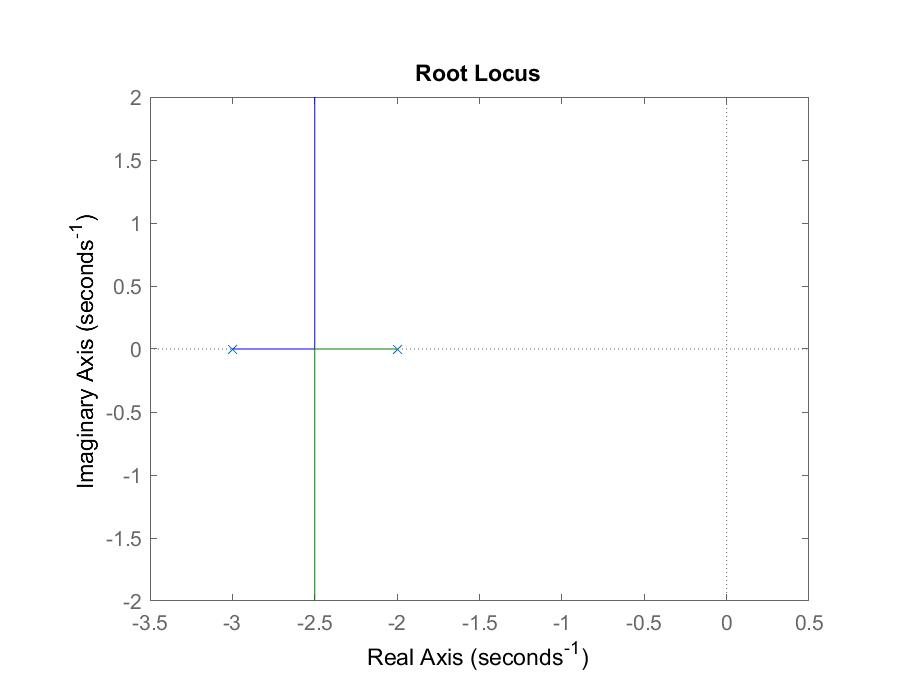
\includegraphics[width=8cm]{wmlocus.eps}}
	\subfloat[Función de transferecia para la planta]{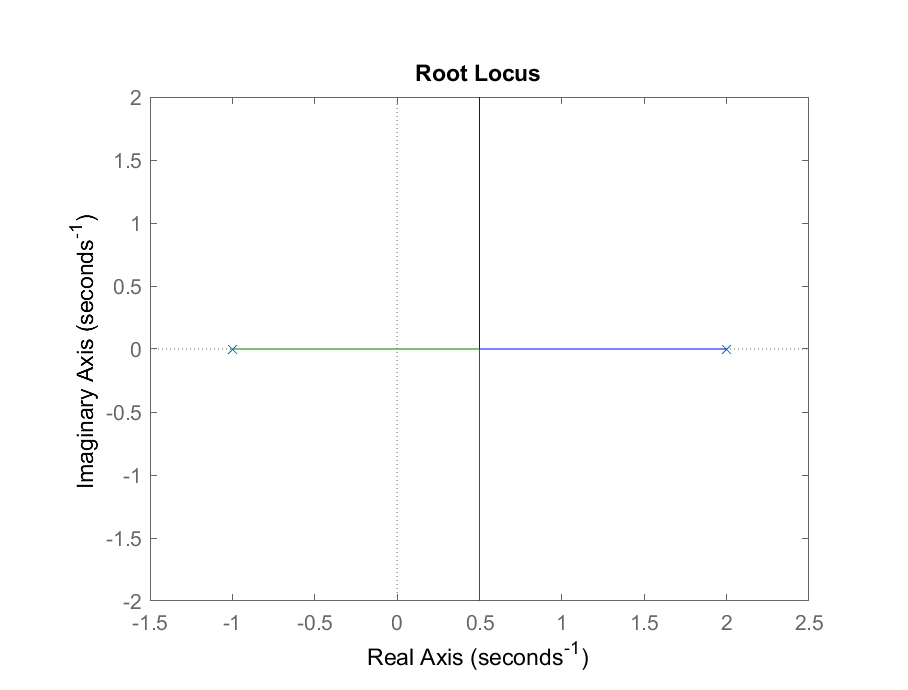
\includegraphics[width=8cm]{wplocus.eps}}
	\caption{Localización de las raíces de los sistemas.}
	\label{locus}
\end{figure}

\begin{figure}[h]
	\centering
	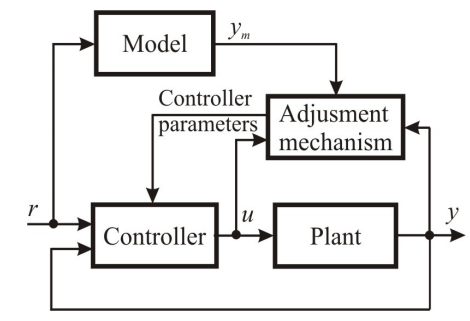
\includegraphics[width=8cm]{general.png}
	\caption{Diagrama de bloques general de MRAS.}
	\label{control}
\end{figure}
De lo anterior, se analiza desde el punto de vista en donde solo se conoce los polinomios $Z_m(s)$ y $Z_p(s)$, es decir, $Z_m(s) = Z_p(s) = 1$. Luego, recordando las leyes de control para $n^* = 1$, la ley de control es definido por,
\begin{align}
\dot{\omega}_2(t) &= \Lambda \omega_2(t) + \ell y_p(t) \nonumber\\
u(t) &= k(t)r(t) + \theta_0(t) y_p(t) + \theta_2^T (t) \omega_2(t) 
\label{ley de control}
\end{align}
donde $\theta_0: \mathbb{R}^+ \rightarrow \mathbb{R}$, $\omega_2, \theta_2: \mathbb{R}^+ \rightarrow \mathbb{R}^{n-1}$, $\Lambda$ es una matriz de $(n-1)\times(n-1)$ asintoticamente estable con $\lambda(s)$ como su polinomio característico y $(\Lambda, \ell)$ es controlable. Las leyes de ajuste son,
\begin{align}
	k(t)  &= \dot{\psi}(t) = -\mathrm{sgn}(k_p) e_1(t)r(t) \nonumber\\
	\dot{\theta}_0(t)  &= \dot{\phi}_0(t) = -\mathrm{sgn}(k_p) e_1(t) y_p(t) \nonumber\\
	\dot{\theta}_2(t) &= \dot{\phi}_2(t) = -\mathrm{sgn}(k_p) e_1(t) \omega_2(t) 
\end{align}

Donde, $e_1 = y_p - y_m$ y $\omega_2(t)$ es definida en \eqref{ley de control} y que puede ser expresada como su transformada de Lagrange,
\begin{equation}
	\omega_2(s) = \frac{\ell}{s - \Lambda} y_p(s)
\end{equation}
La implementación de este control se muestra en la Figura \ref{controlsimple}.
\begin{figure}[h]
	\centering
	\captionsetup{justification=centering}
	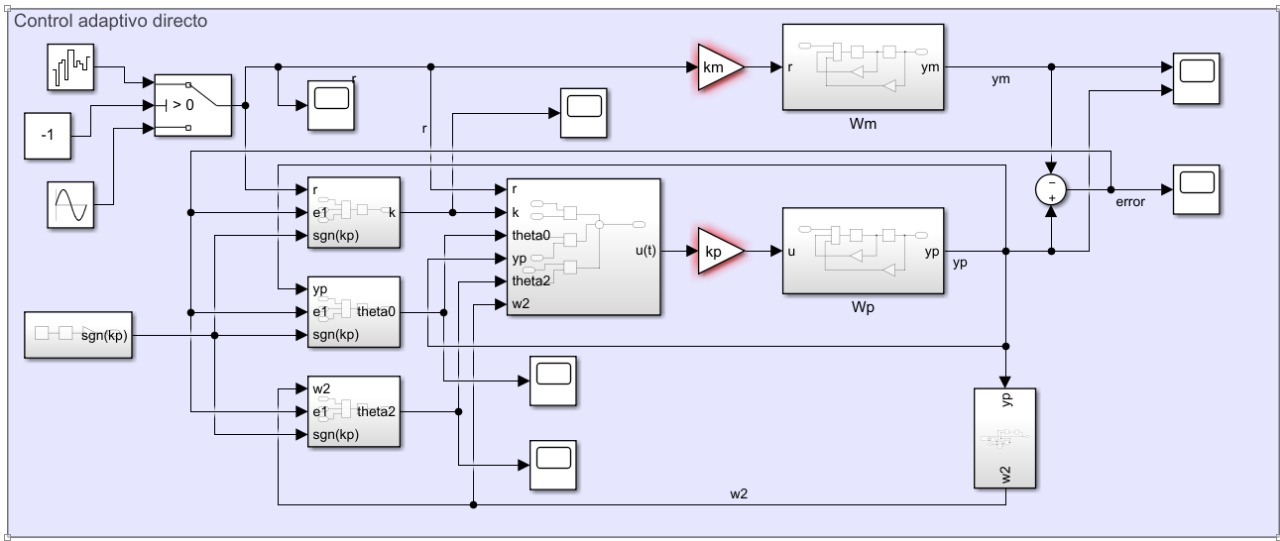
\includegraphics[width=15cm]{controlsimple.png}
	\caption{Diagrama de bloque del sistema controlado por 3 leyes de ajuste para $n^* = 1$.}
	\label{controlsimple}
\end{figure}



Si bien este sistema funciona para entradas tipo ruido y señales sinusoidales, se introduce un termino conocido como $Tuner$, en donde la generación del control de $u(t)$ puede ser convencionalmente descrita por un controlador y el tuner. La forma es lineal e invariante en el tiempo para valores constante de los parámetros de control del vector $\theta$. De esta forma, la ley de control esta definida como,
\begin{align}
	\dot{\omega}_1(t) &= \Lambda \omega_1(t) + \ell u(t) \nonumber \\
	\dot{\omega}_2(t) &= \Lambda \omega_2(t) + \ell y_p(t) \nonumber \\
	\omega(t) &= [r(t), \omega_1^T(t), y_p(t), \omega_2^T(t)]^T \nonumber \\
	\theta(t) &= [k(t), \theta_1^T(t), \theta_0(t), \theta_2^T(t)]^T \nonumber \\
	u(t) &= \theta^T \omega(t)
	\label{vector}
\end{align}

Las leyes de ajuste para generar la ley de control se presentan a continuación, por otro lado, se añade un termino de ganancia $\gamma$ a cada ley,
\begin{align}
	k(t)  &= \dot{\psi}(t) = -\gamma_1 \cdot \mathrm{sgn}(k_p) e_1(t)r(t) \nonumber\\
	\dot{\theta}_0(t)  &= \dot{\phi}_0(t) = -\gamma_2 \cdot\mathrm{sgn}(k_p) e_1(t) y_p(t) \nonumber\\
	\dot{\theta}_1(t)  &= \dot{\phi}_1(t) = -\gamma_3\cdot\mathrm{sgn}(k_p) e_1(t) \omega_1(t) \nonumber\\
	\dot{\theta}_2(t) &= \dot{\phi}_2(t) = -\gamma_4\cdot\mathrm{sgn}(k_p) e_1(t) \omega_2(t) 
	\label{leyes1}
\end{align}

Los valores de $\omega_1(t)$ y $\omega_2$ se pueden expresar como,
\begin{align}
	\omega_1(s) = \frac{\ell}{s - \Lambda} u(s) \nonumber \\
	\omega_2(s) = \frac{\ell}{s - \Lambda} y_p(s)
\end{align}

Hasta aquí lo anterior es valido para $n^*=1$ y es presentado porque las leyes de ajuste y de control se mantienen casi de la misma forma con pequeñas modificaciones.   

La primera de ellas nace del uso de la identidad de Bezout, donde se puede demostrar que existe un vector de control $\theta(t) = \theta^*$ tal que la función de transferencia del sistema completo $W_o(s)$ sea igual al modelo de referencia $W_m(s)$. Se define $\lambda(s)$ como un polinomio mónico como,
\begin{equation}
\lambda(s) = Z_m(s)\lambda_1(s)
\end{equation}
donde $\lambda_1(s)$ es un polinomio de Hurwitz de grado $(n-m-1)=1$, es decir, $\lambda_1 = s+1$. Luego, la función de transferencia del sistema completo es,
\begin{equation}
	W_o(s) = \frac{k_c k_p Z_p(s) \lambda_1(s) Z_m(s)}{R_p(s)[\lambda(s) - C(s)] - k_p Z_p(s) D(s)}	
\label{Wo}
\end{equation}
La existencia de los parámetros de control del vector $\theta^*$ es equivalente a la existencia de los polinomios $C(s)$ y $D(s)$ (o equivalente a ($\lambda(s) - C(s)$) y $D(s)$) tal que el denominador del polinomio de la ecuación \eqref{Wo} pueda ser igual a $Z_p(s)\lambda_1(s)R_m(s)$. Con la identidad de Bezout se identifica $R_p(s)$ con $Q(s)$, $-k_p Z_p(s) $ con $P(s)$ y $Z_p(s) \lambda_1(s)R_m(s)$ con $Q^*(s)$ como la ecuación \eqref{QQ}. Luego, el problema se basa en determinar $C^*(s)$ y $D^*(s)$ tal que $W_o(s) = W_m(s)$ que resulta en,
\begin{equation}
	[\lambda(s) - C^*(s)]Q(s) + D^*(s) P(s) = Q^*(s)
\end{equation}
y 
\begin{align}
k_c = k^* = \frac{k_m}{k_p}
\end{align}
Como la ecuación tiene la forma mostrada en la ecuación \eqref{lema}, por el lema se demuestra la existencia de los parámetros de control del vector $\theta^*$. De esta forma se encuentran los valores esperados como sigue,
\begin{align}
[Z_m(s)\lambda_1(s) - \theta_1^*]R_p - k_p Z_p[\theta_2^* + \theta_0^* Z_m(s)\lambda_1(s)] &= Z_p \lambda_1(s) R_m \nonumber \\
[(1)(s + 1) - \theta_1^*] [s^2 - s - 2] - 3 (1)[\theta_2^* + \theta_0^* (1)(s + 1)] &= (1) (s + 1) [s^2 + 5s + 6]\nonumber \\
[(s + (1 - \theta_1^*)] [s^2 - s - 2] - 3[\theta_2^* + \theta_0^*(s + 1)] &= [s^3 + 6s^2 + 11s + 6]\nonumber \\
s^3 + s^2(-\theta_1^*) + s(\theta_1^* -3 - 3\theta_0^*) + (2\theta_1^* - 2 - 3\theta_2^* - 3\theta_0^*) &= s^3 + 6s^2 + 11s + 6
\end{align}
Resultando en,
\begin{align}
	k^* &= 1.33\nonumber \\
	\theta_1^* &= -6 \nonumber \\
	\theta_0^* &= -6.67 \nonumber \\
	\theta_2^* &= 0
\end{align}


Volviendo a la ecuación \eqref{leyes1} de las leyes de control $\theta(t)$, se reemplaza el error $e_1(t)$ por el error aumentado definido como $\varepsilon = e_1(t) + k_1(t)e_2(t)$ con $e_2(t) = \theta^T \bar{\omega} - \bar{u}$ representando hasta ahora lo que es el control adaptativo directo de un sistema de grado relativo $n^* \geq 2$ como muestra el diagrama general de la Figura \ref{control1} y $k_1^* = k_p/k_m$.

\begin{figure}[h]
	\centering
	\captionsetup{justification=centering}
	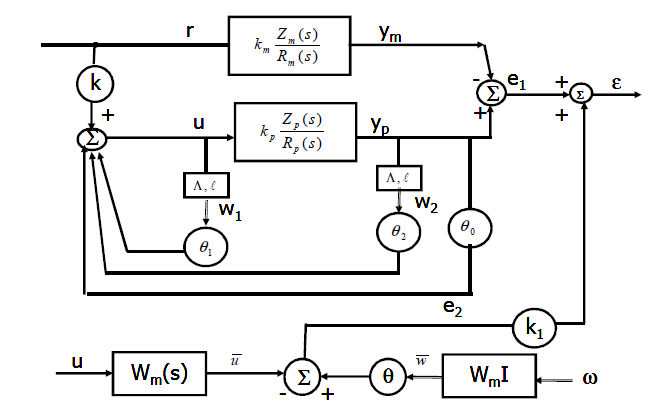
\includegraphics[width=10cm]{control2.png}
	\caption{Diagrama de bloques representativo del control adaptativo para un sistema de grado relativo igual a $2$.}
	\label{control1}
\end{figure}

Expresando los términos de manera más explicita, se tiene,
\begin{align}
	e_2(t) &= [\theta^T W_m(s) I - W_m (s)\theta^T]\omega \nonumber \\
	\varepsilon &= \frac{1}{k^*} \phi^T \zeta + \psi_1 e_2  \nonumber \\
	\zeta &= W_m(s)I \omega \nonumber \\
	\dot{\theta} &= \dot{\phi} =  -\gamma \cdot\mathrm{sgn}(k_p) \frac{\varepsilon \zeta}{1 + \bar{\zeta}^T \bar{\zeta}}\nonumber \\
	\dot{\psi}_1 &= -\gamma_5\cdot\frac{\varepsilon e_2}{1 + \bar{\zeta}^T \bar{\zeta}}\nonumber \\
	\bar{\zeta} &= W_m(s)I \bar{\omega}
\end{align}
con $I$ como la matriz de identidad de dimensión  $ (2n-1)\times(2n - 1)$. La ecuación \eqref{vector} se le añaden los siguientes términos,
\begin{align}
	\omega(t) &= [r(t), \omega_1^T(t), y_p(t), \omega_2^T(t)]^T \nonumber \\
	\theta(t) &= [k(t), \theta_1^T(t), \theta_0(t), \theta_2^T(t)]^T \nonumber \\
	\bar{\theta} &= [k(t),\ \theta_1^T, \theta_0, \theta_2^T]^T\nonumber\\
	\bar{\omega} &= [r(t),\ \omega_1^T, y_p, \omega_2^T]^T  
\end{align}
con los parámetros de error definidos como,
\begin{align}
		\psi_1(t) &= k_1(t) - k_1^* \nonumber \\
		\psi(t) &= k(t) - k^* \nonumber \\
		\phi_0 &= \theta_0(t) - \theta_0^* \nonumber \\
		\phi_1 &= \theta_1(t) - \theta_1^* \nonumber \\
		\phi_2 &= \theta_2(t) - \theta_2^* \nonumber \\
		\phi(t) &= [\psi, \phi_1^T, \phi_0, \phi_2^T]^T 
\end{align}

La representación de todo lo anterior se puede ver en el diagrama de la Figura \ref{errordiagrama}.

\begin{figure}[h]
	\centering
	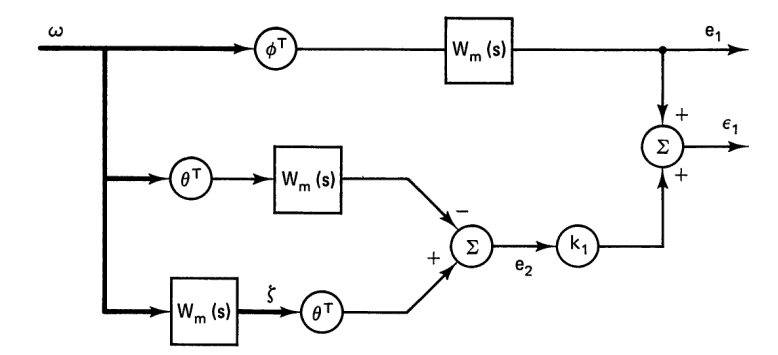
\includegraphics[width=10cm]{error.png}
	\caption{Error aumentado para $k_p$ desconocido con $n^* =2$.}
	\label{errordiagrama}
\end{figure}

Finalmente, al diagrama de bloques mostrado en la Figura \ref{controlsimple} debe ser modificado, terminando como se muestra en las Figuras,
\begin{figure}
	\centering
	\captionsetup{justification=centering}
	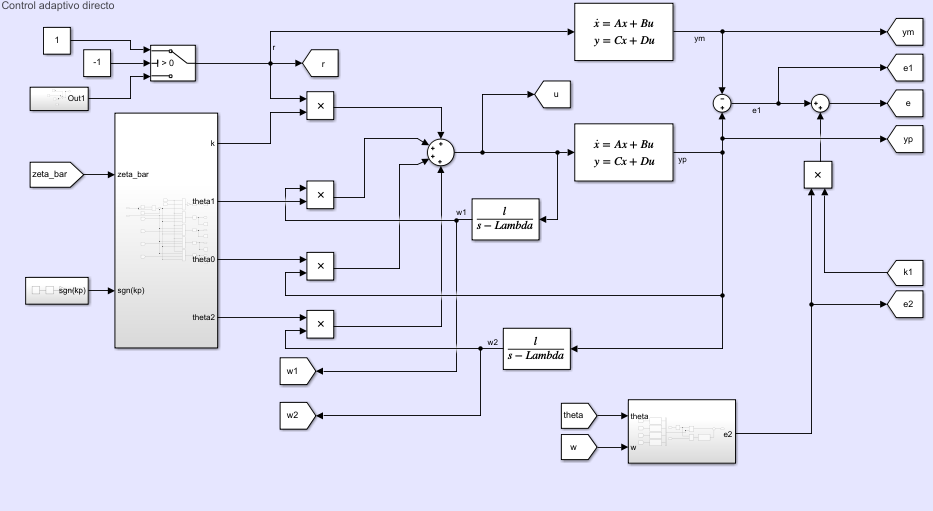
\includegraphics[width=14cm]{control_real.png}
	\caption{Diagrama de bloques para un control adaptativo directo de un sistema de grado relativo $n^* = 2$.}
	\label{controlreal}.
\end{figure}
\begin{figure}
	\centering
	\captionsetup{justification=centering}
	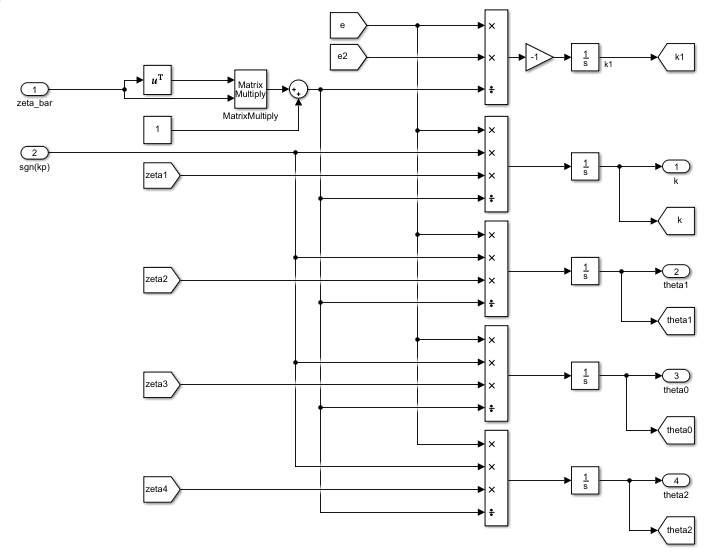
\includegraphics[width=10cm]{leyesajuste.png}
	\caption{Diagrama de bloques para las leyes de ajuste del control adaptativo.}
	\label{leyesdeajuste}.
\end{figure}
\begin{figure}
	\centering
	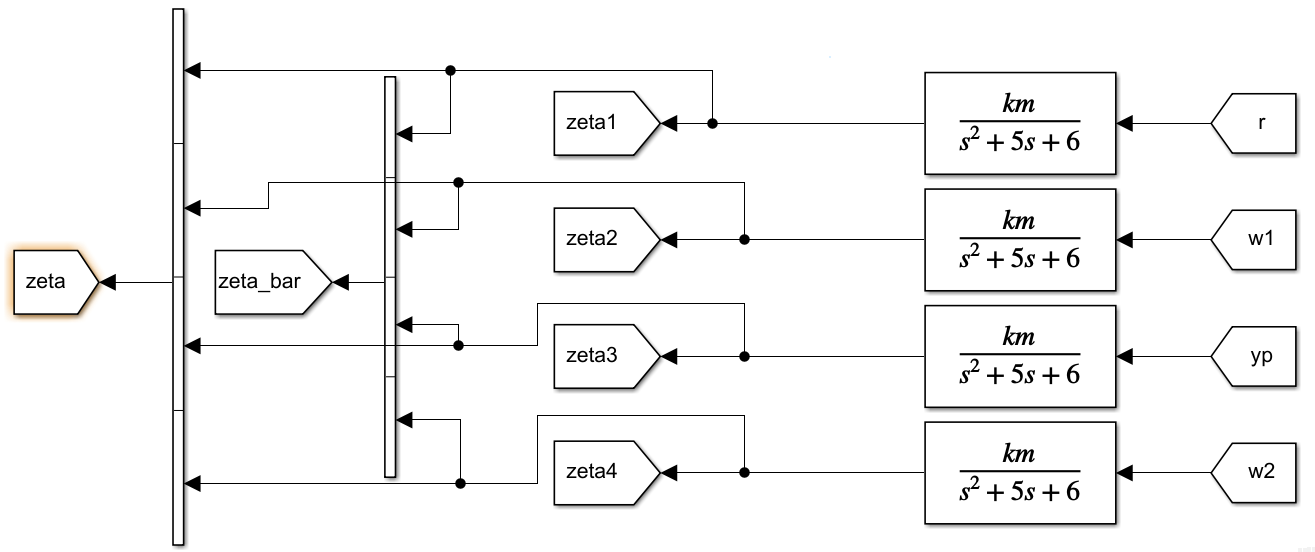
\includegraphics[width=14cm]{vectorauxiliar.png}
	\caption{Diagrama de bloques para los vectores auxiliares.}
	\label{vectorauxiliar}.
\end{figure}
\begin{figure}
	\centering
	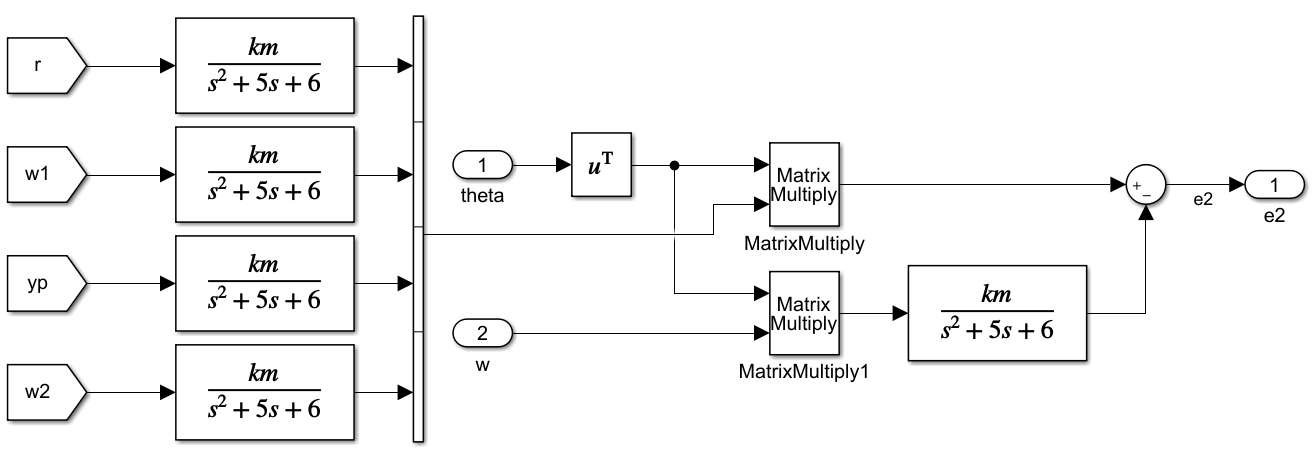
\includegraphics[width=14cm]{error2.png}
	\caption{Diagrama de bloques para calcular el error aumentado.}
	\label{error2}.
\end{figure}

\subsection{Experimentos con diferentes parámetros}
\subsubsection{Condiciones iniciales diferentes entrada oscilante}
Primero, se muestran los resultados para las condiciones iniciales dadas en el enunciado. La entrada es $r(t) = 2\sin((5)t) + \sin((1)t) + \sin( (10)t)$ que corresponde a una entrada de excitación persistente con 3 frecuencias diferentes de un mínimo de $n/2$ donde $n$ es el numero de variables a ajustar. Los resultados se muestran en la columna de la Figura \ref{inicialrs}.(a) junto con los demás experimento que se detallan a continuación:
\begin{itemize}
	\item Para una condición inicial $y_m = 5$ y $\dot{y}_p = 1$. Columna de la Figura \ref{inicialrs}.(b)
	\item Para $\dot{y}_m = 5$ y $\dot{y}_p = 5$. Columna de la Figura \ref{inicialrs}.(c)
\end{itemize}

\newpage
\begin{figure}[h]
	\centering
	\captionsetup{justification=centering}
	\subfloat {\includegraphics[width=6cm]{c0error.eps}}
	\subfloat {\includegraphics[width=6cm]{c1error.eps}}
	\subfloat {\includegraphics[width=6cm]{c2error.eps}}
	\newline
	\noindent
	\subfloat {\includegraphics[width=6cm]{c0respuesta.eps}}
	\subfloat {\includegraphics[width=6cm]{c1respuesta.eps}}
	\subfloat {\includegraphics[width=6cm]{c2respuesta.eps}}
	\newline
	\noindent
	\stepcounter{figure}\addtocounter{figure}{-1}  
	\subfloat[]{\includegraphics[width=6cm]{c0leyes.eps}}
	\subfloat[]{\includegraphics[width=6cm]{c1leyes.eps}}
	\subfloat[]{\includegraphics[width=6cm]{c2leyes.eps}}
	\caption{Resultados de simulaciones para diferentes valores iniciales del sistema con entrada oscilante.}
	\label{inicialrs}
\end{figure}

\subsubsection{Condiciones iniciales diferentes entrada unitaria}
Primero, se muestran los resultados para las condiciones iniciales dadas en el enunciado. La entrada es $r(t) = 1$. Los resultados se muestran en la columna de la Figura \ref{inicialrl}.(a) junto con los demás experimento que se detallan a continuación:
\begin{itemize}
	\item Para una condición inicial $y_m = 5$ y $\dot{y}_p = 1$. Columna de la Figura \ref{inicialrl}.(b)
	\item Para $\dot{y}_m = 5$ y $\dot{y}_p = 5$. Columna de la Figura \ref{inicialrl}.(c)
\end{itemize}
\newpage
\begin{figure}[h]
	\centering
	\captionsetup{justification=centering}
	\subfloat {\includegraphics[width=6cm]{c3error.eps}}
	\subfloat {\includegraphics[width=6cm]{c4error.eps}}
	\subfloat {\includegraphics[width=6cm]{c5error.eps}}
	\newline
	\noindent
	\subfloat {\includegraphics[width=6cm]{c3respuesta.eps}}
	\subfloat {\includegraphics[width=6cm]{c4respuesta.eps}}
	\subfloat {\includegraphics[width=6cm]{c5respuesta.eps}}
	\newline
	\noindent\\
	\stepcounter{figure}\addtocounter{figure}{-1}  
	\subfloat[]{\includegraphics[width=6cm]{c3leyes.eps}}
	\subfloat[]{\includegraphics[width=6cm]{c4leyes.eps}}
	\subfloat[]{\includegraphics[width=6cm]{c5leyes.eps}}
	\caption{Resultados de simulaciones para diferentes valores iniciales del sistema con entrada unitaria.}
	\label{inicialrl}
\end{figure}

\subsubsection{Variación de ganancias adaptativas con entrada unitaria}
Parámetros:
\begin{itemize}
	\item Todas las ganancias $\gamma_i = 0.1$. Columna de la Figura \ref{gananciasrl}.(a)
	\item Todas las ganancias $\gamma_i = 1.0$. Columna de la Figura \ref{gananciasrl}.(b)
	\item Todas las ganancias $\gamma_i = 10$. Columna de la Figura \ref{gananciasrl}.(c)
\end{itemize}
\newpage
\begin{figure}[h]
	\centering
	\captionsetup{justification=centering}
	\subfloat{\includegraphics[width=6cm]{c6error.eps}}
	\subfloat{\includegraphics[width=6cm]{c7error.eps}}
	\subfloat{\includegraphics[width=6cm]{c8error.eps}}
	\newline
	\noindent
	\subfloat{\includegraphics[width=6cm]{c6respuesta.eps}}
	\subfloat{\includegraphics[width=6cm]{c7respuesta.eps}}
	\subfloat{\includegraphics[width=6cm]{c8respuesta.eps}}
	\newline
	\noindent
	\stepcounter{figure}\addtocounter{figure}{-1}  
	\subfloat[]{\includegraphics[width=6cm]{c6leyes.eps}}
	\subfloat[]{\includegraphics[width=6cm]{c7leyes.eps}}
	\subfloat[]{\includegraphics[width=6cm]{c8leyes.eps}}
	\caption{Resultados de simulaciones para diferentes valores de ganancia adaptativa con una entrada unitaria.}
	\label{gananciasrl}
\end{figure}

\subsubsection{Variación de ganancias adaptativas con entrada oscilante}
Parámetros:
\begin{itemize}
	\item Todas las ganancias $\gamma_i = 0.1$. Columna de la Figura \ref{gananciasrs}.(a)
	\item Todas las ganancias $\gamma_i = 1.0$. Columna de la Figura \ref{gananciasrs}.(b)
	\item Todas las ganancias $\gamma_i = 10$. Columna de la Figura \ref{gananciasrs}.(c)
\end{itemize}
\newpage
\begin{figure}[h]
	\centering
	\captionsetup{justification=centering}
	\subfloat{\includegraphics[width=6cm]{c9error.eps}}
	\subfloat{\includegraphics[width=6cm]{c10error.eps}}
	\subfloat{\includegraphics[width=6cm]{c11error.eps}}
	\newline
	\noindent
	\subfloat{\includegraphics[width=6cm]{c9respuesta.eps}}
	\subfloat{\includegraphics[width=6cm]{c10respuesta.eps}}
	\subfloat{\includegraphics[width=6cm]{c11respuesta.eps}}
	\newline
	\noindent
	\stepcounter{figure}\addtocounter{figure}{-1}  
	\subfloat[]{\includegraphics[width=6cm]{c9leyes.eps}}
	\subfloat[]{\includegraphics[width=6cm]{c10leyes.eps}}
	\subfloat[]{\includegraphics[width=6cm]{c11leyes.eps}}
	\caption{Resultados de simulaciones para diferentes valores de ganancia adaptativa con una entrada oscilante.}
	\label{gananciasrs}
\end{figure}
\subsubsection{Variación de ganancias adaptativas con entrada ruido blanco}
Parámetros:
\begin{itemize}
	\item Todas las ganancias $\gamma_i = 0.1$. Columna de la Figura \ref{gananciasruido}.(a)
	\item Todas las ganancias $\gamma_i = 1.0$. Columna de la Figura \ref{gananciasruido}.(b)
	\item Todas las ganancias $\gamma_i = 10$. Columna de la Figura \ref{gananciasruido}.(c)
\end{itemize}
\newpage
\begin{figure}[h]
	\centering
	\captionsetup{justification=centering}
	\subfloat{\includegraphics[width=6cm]{c12error.eps}}
	\subfloat{\includegraphics[width=6cm]{c13error.eps}}
	\subfloat{\includegraphics[width=6cm]{c14error.eps}}
	\newline
	\noindent
	\subfloat{\includegraphics[width=6cm]{c12respuesta.eps}}
	\subfloat{\includegraphics[width=6cm]{c13respuesta.eps}}
	\subfloat{\includegraphics[width=6cm]{c14respuesta.eps}}
	\newline
	\noindent
	\stepcounter{figure}\addtocounter{figure}{-1}  
	\subfloat[]{\includegraphics[width=6cm]{c12leyes.eps}}
	\subfloat[]{\includegraphics[width=6cm]{c13leyes.eps}}
	\subfloat[]{\includegraphics[width=6cm]{c14leyes.eps}}
	\caption{Simulaciones para diferentes valores de ganancia adaptativa con ruido blanco.}
	\label{gananciasruido}
\end{figure}
\subsubsection{Variación del parámetro $b_p$ de la planta con entrada unitaria}
Recordando solo el denominador $R_p$ de la función de transferencia de la planta, definido como $R_p(s) = s^2 + b_ps + c_p$ con $b_p=-1$ y $c_p = -2$, se presentan 3 simulaciones. Los parámetros $k^*, \theta_1^*, \theta_0^*, \theta_2^*$, son reajustados internamente.
\begin{itemize}
	\item Parámetro $b_p = 5$. Columna de la Figura \ref{parametrob}.(a)
	\item Parámetro $b_p = 0$. Columna de la Figura \ref{parametrob}.(b)
	\item Parámetro $b_p = -5$. Columna de la Figura \ref{parametrob}.(c)
\end{itemize}
\newpage

\begin{figure}[h]
	\centering
	\captionsetup{justification=centering}
	\subfloat{\includegraphics[width=6cm]{c15error.eps}}
	\subfloat{\includegraphics[width=6cm]{c16error.eps}}
	\subfloat{\includegraphics[width=6cm]{c17error.eps}}
	\newline
	\noindent
	\subfloat{\includegraphics[width=6cm]{c15respuesta.eps}}
	\subfloat{\includegraphics[width=6cm]{c16respuesta.eps}}
	\subfloat{\includegraphics[width=6cm]{c17respuesta.eps}}
	\newline
	\noindent
	\stepcounter{figure}\addtocounter{figure}{-1}  
	\subfloat[]{\includegraphics[width=6cm]{c15leyes.eps}}
	\subfloat[]{\includegraphics[width=6cm]{c16leyes.eps}}
	\subfloat[]{\includegraphics[width=6cm]{c17leyes.eps}}
	\caption{Resultados de simulaciones para diferentes valores de $b_p$ con una entrada unitaria.}
	\label{parametrob}
\end{figure}
\subsubsection{Variación del parámetro $c_p$ de la planta con entrada unitaria}
Recordando solo el denominador $R_p$ de la función de transferencia de la planta, definido como $R_p(s) = s^2 + b_ps + c_p$ con $b_p=-1$ y $c_p = -2$, se presentan 3 simulaciones,
\begin{itemize}
	\item Parámetro $c_p = 5$. Columna de la Figura \ref{parametroc}.(a)
	\item Parámetro $c_p = 0$. Columna de la Figura \ref{parametroc}.(b)
	\item Parámetro $c_p = -5$. Columna de la Figura \ref{parametroc}.(c)
\end{itemize}
Las condiciones iniciales son las del enunciado y las ganancias adaptativas son igual a la unidad.
\newpage
\begin{figure}[h]
	\centering
	\captionsetup{justification=centering}
	\subfloat{\includegraphics[width=6cm]{c18error.eps}}
	\subfloat{\includegraphics[width=6cm]{c19error.eps}}
	\subfloat{\includegraphics[width=6cm]{c20error.eps}}
	\newline
	\noindent
	\subfloat{\includegraphics[width=6cm]{c18respuesta.eps}}
	\subfloat{\includegraphics[width=6cm]{c19respuesta.eps}}
	\subfloat{\includegraphics[width=6cm]{c20respuesta.eps}}
	\newline
	\noindent
	\stepcounter{figure}\addtocounter{figure}{-1}  
	\subfloat[]{\includegraphics[width=6cm]{c18leyes.eps}}
	\subfloat[]{\includegraphics[width=6cm]{c19leyes.eps}}
	\subfloat[]{\includegraphics[width=6cm]{c20leyes.eps}}
	\caption{Resultados de simulaciones para diferentes valores de $c_p$ con una entrada unitaria.}
	\label{parametroc}
\end{figure}
\subsubsection{Variación del parámetro $b_p$ de la planta con entrada oscilante}
La entrada es $r(t) = 2\sin((5)t) + \sin((1)t) + \sin((10)t)$ y la simulaciones son:
\begin{itemize}
	\item Parámetro $b_p = 5$. Columna de la Figura \ref{parametrobO}.(a)
	\item Parámetro $b_p = 0$. Columna de la Figura \ref{parametrobO}.(b)
	\item Parámetro $b_p = -5$. Columna de la Figura \ref{parametrobO}.(c)
\end{itemize}
Las condiciones iniciales son las del enunciado y las ganancias adaptativas son igual a la unidad.
\newpage
\begin{figure}[h]
	\centering
	\captionsetup{justification=centering}
	\subfloat{\includegraphics[width=6cm]{c21error.eps}}
	\subfloat{\includegraphics[width=6cm]{c22error.eps}}
	\subfloat{\includegraphics[width=6cm]{c23error.eps}}
	\newline
	\noindent
	\subfloat{\includegraphics[width=6cm]{c21respuesta.eps}}
	\subfloat{\includegraphics[width=6cm]{c22respuesta.eps}}
	\subfloat{\includegraphics[width=6cm]{c23respuesta.eps}}
	\newline
	\noindent
	\stepcounter{figure}\addtocounter{figure}{-1}  
	\subfloat[]{\includegraphics[width=6cm]{c21leyes.eps}}
	\subfloat[]{\includegraphics[width=6cm]{c22leyes.eps}}
	\subfloat[]{\includegraphics[width=6cm]{c23leyes.eps}}
	\caption{Resultados de simulaciones para diferentes valores de $b_p$ con una entrada oscilante.}
	\label{parametrobO}
\end{figure}
\subsubsection{Variación del parámetro $c_p$ de la planta con entrada oscilante}
La entrada es $r(t) = 2\sin((5)t) + \sin((1)t) + \sin((10)t)$ y la simulaciones son:
\begin{itemize}
	\item Parámetro $c_p = 5$. Columna de la Figura \ref{parametrocO}.(a)
	\item Parámetro $c_p = 0$. Columna de la Figura \ref{parametrocO}.(b)
	\item Parámetro $c_p = -5$. Columna de la Figura \ref{parametrocO}.(c)
\end{itemize}
Las condiciones iniciales son las del enunciado y las ganancias adaptativas son igual a la unidad.
\newpage
\begin{figure}[h]
	\centering
	\captionsetup{justification=centering}
	\subfloat{\includegraphics[width=6cm]{c24error.eps}}
	\subfloat{\includegraphics[width=6cm]{c25error.eps}}
	\subfloat{\includegraphics[width=6cm]{c26error.eps}}
	\newline
	\noindent
	\subfloat{\includegraphics[width=6cm]{c24respuesta.eps}}
	\subfloat{\includegraphics[width=6cm]{c25respuesta.eps}}
	\subfloat{\includegraphics[width=6cm]{c26respuesta.eps}}
	\newline
	\noindent
	\stepcounter{figure}\addtocounter{figure}{-1}  
	\subfloat[]{\includegraphics[width=6cm]{c24leyes.eps}}
	\subfloat[]{\includegraphics[width=6cm]{c25leyes.eps}}
	\subfloat[]{\includegraphics[width=6cm]{c26leyes.eps}}
	\caption{Resultados de simulaciones para diferentes valores de $c_p$ con una entrada oscilante.}
	\label{parametrocO}
\end{figure}

De los últimos gráficos se puede concluir que es muy importante conocer los valores de la planta o tener un estimado de ella ya que si éste varia, puede cambiar por completo la respuesta del error y las leyes de ajuste podrían no converger nunca a un valor. Por otro lado, se vio que cuando existen perturbaciones como ruido blanco, influyen en el comportamiento de las leyes de ajuste inclusive en el largo plazo.\\
Por estos motivos, en la siguiente sección de la tarea se analiza como deben cambiar las leyes de ajuste ante perturbaciones en la salida de la planta y ante valores de la planta variables en el tiempo.

\newpage
\section{Problema 2}
\begin{enumerate}[]
\item Considere la planta inestable y desconocida de segundo orden de la Parte A. Suponga ahora que actúa una perturbación externa $p(t)$ sobre la salida del sistema. Modifique el diseño del controlador para tomar en cuenta dicha perturbación y lograr que la salida de la planta permanezca lo más parecida posible a la salida del modelo de referencia.

Estudiar los casos en que se aplica una perturbación constante de amplitud $P$ y una senoidal de amplitud $A$ y frecuencia $\omega$ en torno al valor medio cero. Estudie la influencia de los parámetros correspondientes de las perturbaciones.

\item Realice el mismo estudio de la parte anterior pero suponiendo ahora que el parámetro 2 de la planta es variante en el tiempo. Considere los casos de variaciones del tipo rampa de pendiente $p$ y duración finita y variaciones sinusoidales de amplitud $A$ y frecuencia $\omega$ alrededor del valor 2. Estudie la influencia de los parámetros correspondientes de las perturbaciones.
\end{enumerate}

\subsection{Solución problema 1}

Una perturbación en la salida se representa como se muestra en el diagrama general de la Figura \ref{plantaperturbacion}.
\begin{figure}[h]
	\centering
	\includegraphics[width=14cm]{plantaperturbacion.png}
	\caption{Perturbación $p(t)$ agregada en la salida de la planta.}
	\label{plantaperturbacion}
\end{figure}


Antes de detallar la solución, se debe remarcar que hay dos escenarios críticos en los cuales se generan modificaciones en las leyes de ajuste ante perturbaciones. Estos son: Cuando la entrada es de excitación persistente y cuando no lo es. Si la excitación es persistente solo se requiere aumentar el grado de la excitación. Sin embargo, cuando $r(t)$ no es excitación persistente es necesario aplicar otros métodos para que las leyes de ajuste puedan converger a un valor cercano a cero. Se realiza un experimento con entrada $r(t) = 2\sin((5)t)$ mostrado en la Figura \ref{estado1}.(a) y otro con entrada unitaria mostrando en la Figura \ref{estado1}.(b). En  ambos casos se realiza para diferentes valores de perturbación constante.\\
\begin{figure}[h]
	\centering
	\captionsetup{justification=centering}
	\subfloat[$r(t) = 2\sin((5)t)$]{\includegraphics[width=0.4\textwidth]{c27todos.eps}}
	\subfloat[$r(t)=1$]{\includegraphics[width=0.4\textwidth]{c28todos.eps}}
	\caption{Comportamiento de las leyes de ajuste para diferentes valores de perturbación constante.}
	\label{estado1}
\end{figure}

Considerando las entradas ya mencionadas, se ve el resultado de aplicar una perturbación oscilatoria definida como $ P =A\cdot \sin(\omega_f t)$ para diferentes valores de $A$ y $\omega_f$. En los gráficos de la Figura \ref{estado2} se puede ver el comportamiento del sistema para diferentes valores de amplitud $A$ mientras que en la Figura \ref{estado3} se puede ver el comportamiento para diferentes valores de $\omega_f$.  
\newpage
\begin{figure}[h]
	\centering
	\captionsetup{justification=centering}
	\subfloat[$r(t) = 2\sin((5)t)$]{\includegraphics[width=0.4\textwidth]{c29todos.eps}}
	\subfloat[$r(t)=1$]{\includegraphics[width=0.4\textwidth]{c30todos.eps}}
	\caption{Comportamiento de las leyes de ajuste para diferentes valores  de amplitud en la perturbación con $\omega_f=2$.}
	\label{estado2}
\end{figure}
\newpage
\begin{figure}[h]
	\centering
	\captionsetup{justification=centering}
	\subfloat[$r(t) = 2\sin((5)t)$]{\includegraphics[width=0.4\textwidth]{c31todos.eps}}
	\subfloat[$r(t)=1$]{\includegraphics[width=0.4\textwidth]{c32todos.eps}}
	\caption{Comportamiento de las leyes de ajuste para diferentes frecuencias en la perturbación con $A = 1$.}
	\label{estado3}
\end{figure}
Durante las simulaciones se observo que los valores iniciales de los parámetros de error son elementos críticos a la hora de analizar el comportamiento del error de la planta $e_1$ y las leyes de ajuste. En los casos anteriores se utilizaron valores iniciales random definidos como $k_0=-1$, $\theta_{00} = 1$, $\theta_{10} = -1$, $\theta_{20} = 2$, sin embargo, si se consideran como valores iniciales los valores objetivos $\theta^*$ el resultado es diferente. Esto se puede ver en las Figuras \ref{estado4} a la \ref{estado6}. 
\newpage
\begin{figure}[h]
	\centering
	\captionsetup{justification=centering}
	\subfloat[$r(t) = 2\sin((5)t)$]{\includegraphics[width=0.4\textwidth]{c33todos.eps}}
	\subfloat[$r(t)=1$]{\includegraphics[width=0.4\textwidth]{c34todos.eps}}
	\caption{Leyes de ajuste para diferentes valores de perturbación constante con valor inicial igual al objetivo.}
	\label{estado4}
\end{figure}
\newpage
\begin{figure}[h]
	\centering
	\captionsetup{justification=centering}
	\subfloat[$r(t) = 2\sin((5)t)$]{\includegraphics[width=0.4\textwidth]{c35todos.eps}}
	\subfloat[$r(t)=1$]{\includegraphics[width=0.4\textwidth]{c36todos.eps}}
	\caption{Leyes de ajuste para diferentes valores de amplitud en la perturbación con $\omega_f=2$ y con valor inicial igual al objetivo.}
	\label{estado5}
\end{figure}
\newpage
\begin{figure}[h]
	\centering
	\captionsetup{justification=centering}
	\subfloat[$r(t) = 2\sin((5)t)$]{\includegraphics[width=0.4\textwidth]{c37todos.eps}}
	\subfloat[$r(t)=1$]{\includegraphics[width=0.4\textwidth]{c38todos.eps}}
	\caption{Leyes de ajuste para diferentes frecuencias en la perturbación con $A = 1$ y  con valor inicial igual al objetivo.}
	\label{estado6}
\end{figure}

Hasta aquí se puede observar que en ocasiones el error de la planta tiende a cero pero en otras tiende a oscilar producto de las perturbaciones, lo mismo ocurre con los valores de las leyes de ajuste representado por $||\phi||$ donde en ocasiones su valor diverge. Para evitar que estos fenómenos ocurran, se presentan 4 métodos que modifican el actuar de las leyes de ajuste evitando que estas puedan divergir y al mismo tiempo acotar los parámetro de error a valores cercanos a los limites de perturban.

\newpage
\subsubsection{Uso de Zona muerta}
Se define la ley de ajuste con una zona muerta bajo una cota representada por la amplitud del ruido y un valor arbitrario positivo, es decir,
\begin{equation}
	\dot{\phi} = \left\{ \begin{array}{cc}
	 -\mathrm{sgn}(k_p)\frac{\varepsilon \zeta}{1 + \xi^T \xi} & |\varepsilon| \ge \nu_o + \delta \\
	 0 & |\varepsilon| < \nu_o + \delta
	 \end{array}\right.
\end{equation}
donde $\delta$ es un valor arbitrario constante y positivo que en este caso se considera igual a $0.01$ y $\xi = [\zeta^T, \omega^T]^T$. Esto asegura que los parámetros se ajusten solo cuando la magnitud del error aumentado sea mayor que un predeterminado valor que depende de la perturbación. La aplicación de este método se ve en la Figura \ref{deadzone}.
\begin{figure}
	\centering
	\includegraphics[width=15cm]{deadzone.png}
	\caption{Modificación de las leyes de ajuste con el uso de Zona muerta.}
	\label{deadzone}
\end{figure}
Se realizara una serie de simulaciones en las que se comparan las respuestas de los errores en función de la entrada para diferentes valores de perturbación constante y perturbaciones oscilatorias. En las Figuras \ref{estado7}-\ref{estado9} y \ref{estado11} se presentan las respuestas cuando las condiciones iniciales de los parámetros de las leyes de ajuste son igual al valor objetivo $\theta^*$, mientras que en las Figuras \ref{estado8}-\ref{estado10} y \ref{estado12} se presentan las respuestas del error ante condiciones iniciales aleatoria de las leyes de ajuste.
\newpage
\begin{figure}[h]
	\centering
	\captionsetup{justification=centering}
	\subfloat[$r(t) = 2\sin((5)t)$]{\includegraphics[width=0.4\textwidth]{c39todos.eps}}
	\subfloat[$r(t)=1$]{\includegraphics[width=0.4\textwidth]{c40todos.eps}}
	\caption{Leyes de ajuste para diferentes valores de perturbación constante con valor inicial igual al objetivo.}
	\label{estado7}
\end{figure}
\newpage
\begin{figure}[h]
	\centering
	\captionsetup{justification=centering}
	\subfloat[$r(t) = 2\sin((5)t)$]{\includegraphics[width=0.4\textwidth]{c41todos.eps}}
	\subfloat[$r(t)=1$]{\includegraphics[width=0.4\textwidth]{c42todos.eps}}
	\caption{Leyes de ajuste para diferentes valores de perturbación constante con valor inicial aleatorio.}
	\label{estado8}
\end{figure}
\newpage
\begin{figure}[h]
	\centering
	\captionsetup{justification=centering}
	\subfloat[$r(t) = 2\sin((5)t)$]{\includegraphics[width=0.4\textwidth]{c43todos.eps}}
	\subfloat[$r(t)=1$]{\includegraphics[width=0.4\textwidth]{c44todos.eps}}
	\caption{Leyes de ajuste para diferentes valores de amplitud en la perturbación con $\omega_f=2$ y con valor inicial igual al objetivo.}
	\label{estado9}
\end{figure}
\newpage
\begin{figure}[h]
	\centering
	\captionsetup{justification=centering}
	\subfloat[$r(t) = 2\sin((5)t)$]{\includegraphics[width=0.4\textwidth]{c45todos.eps}}
	\subfloat[$r(t)=1$]{\includegraphics[width=0.4\textwidth]{c46todos.eps}}
	\caption{Leyes de ajuste para diferentes valores de amplitud en la perturbación con $\omega_f=2$ y con valor inicial aleatorio.}
	\label{estado10}
\end{figure}
\newpage
\begin{figure}[h]
	\centering
	\captionsetup{justification=centering}
	\subfloat[$r(t) = 2\sin((5)t)$]{\includegraphics[width=0.4\textwidth]{c47todos.eps}}
	\subfloat[$r(t)=1$]{\includegraphics[width=0.4\textwidth]{c48todos.eps}}
	\caption{Leyes de ajuste para diferentes frecuencias en la perturbación con $A = 1$ y  con valor inicial igual al objetivo.}
	\label{estado11}
\end{figure}
\newpage
\begin{figure}[h]
	\centering
	\captionsetup{justification=centering}
	\subfloat[$r(t) = 2\sin((5)t)$]{\includegraphics[width=0.4\textwidth]{c49todos.eps}}
	\subfloat[$r(t)=1$]{\includegraphics[width=0.4\textwidth]{c50todos.eps}}
	\caption{Leyes de ajuste para diferentes frecuencias en la perturbación con $A = 1$ y con valor inicial aleatorio.}
	\label{estado12}
\end{figure}

Se puede notar que cuando los valores iniciales de las leyes de ajuste son muy diferentes de los valores objetivos el sistema tiene una respuesta tardía que incremento demasiado el error de la planta. Sin embargo, a pesar de esto el sistema logra acotar el error y los parámetros en la mayoría de las simulaciones.
\newpage
\subsubsection{Cota sobre $||\theta^*||$}
En este caso el espacio esperado de los parámetros es acotado por el espacio $S$ definido como,
\begin{equation}
	S = \{\theta|\  ||\theta|| \le \theta_{max}^*\}
\end{equation}
donde $\theta_{max}^*$ es una constante positiva. Luego, las leyes de ajuste toman la forma de,
\begin{equation}
	\dot{\phi} = -\mathrm{sgn}(k_p) \frac{\varepsilon \zeta}{1 + \xi^T \xi} - \theta f(\theta)
\end{equation}
con 
\begin{equation}
	f(\theta) = \left\{ \begin{array}{cc}
	\left( 1 - \frac{||\theta||}{\theta_{max}^*}\right) & ||\theta|| > \theta_{max}^*\\
	0 & ||\theta|| \le \theta_{max}^*
	\end{array}\right.
\end{equation}

La implementación de este método se muestra en la Figura \ref{thetamax}.
\begin{figure}
	\centering
	\includegraphics[width=14cm]{thetamax.png}
	\caption{Modificación de las leyes de ajuste acotando el valor de $||\theta||$.}
	\label{thetamax}
\end{figure}
Primero, se analiza la influencia del valor máximo de 
$\theta$ para las dos entradas utilizadas en los ejemplos anteriores para valores iniciales de los parámetros diferentes a los objetivos (que es e peor caso para la cota del error y los parámetros). Los resultados para una entrada oscilatoria y para una entrada unitaria se muestran en la Figura \ref{thetavar}. La perturbación considerada es constante e igual a $5$.\\
Se puede observar que el error del sistema varia en función de la cota. Al escoger un valor de $f(\theta)$ aleatoria el error comienza a crecer ya que los parámetros de la ley de ajuste nunca alcanzan el valor optimo. Por otro lado, es de esperar que si se escoge como $||\theta_{max}||$ como la norma de los valores objetivos, luego el error oscilara alrededor de cero. Sin embargo, esto solo sirve como referencia ya que aún con una norma igual al valor esperada de $||\theta||$ no se tiene certeza de que valor podría tener cada elemento del vector que bien podrían ser diferentes a los esperado. Por ello, el valor se fija en $||\theta_{max}^*|| = 9$ resultando en los gráficos de la Figura \ref{thetaopt}.
\newpage
\begin{figure}[h]
	\centering
	\captionsetup{justification=centering}
	\subfloat[$r(t) = 2\sin((5)t)$]{\includegraphics[width=0.4\textwidth]{c51todos.eps}}
	\subfloat[$r(t)=1$]{\includegraphics[width=0.4\textwidth]{c52todos.eps}}
	\caption{Leyes de ajuste y error para diferentes valores de $\theta_{max}$.}
	\label{thetavar}
\end{figure}
\newpage
\begin{figure}[h]
	\centering
	\captionsetup{justification=centering}
	\subfloat[$r(t) = 2\sin((5)t)$]{\includegraphics[width=0.4\textwidth]{c53todos.eps}}
	\subfloat[$r(t)=1$]{\includegraphics[width=0.4\textwidth]{c54todos.eps}}
	\caption{Leyes de ajuste y error para $\theta_{max}^* = 9$ con perturbación constante y condición inicial de $\theta$ aleatorio.}
	\label{thetaopt}
\end{figure}
Ahora que se conoce el efecto de la cota para los parámetros de las leyes de ajuste se analiza con valores iniciales iguales a los objetivos y así observar más de cerca el valor de $e_1$. El resultado de las simulaciones se agrupan en las Figuras \ref{cota1}-\ref{cota2} y \ref{cota3}.
\newpage
\begin{figure}[h]
	\centering
	\captionsetup{justification=centering}
	\subfloat[$r(t) = 2\sin((5)t)$]{\includegraphics[width=0.4\textwidth]{c55todos.eps}}
	\subfloat[$r(t)=1$]{\includegraphics[width=0.4\textwidth]{c56todos.eps}}
	\caption{Leyes de ajuste y error para $\theta_{max}^* =9$ y perturbación constante.}
	\label{cota1}
\end{figure}
\newpage
\begin{figure}[h]
	\centering
	\captionsetup{justification=centering}
	\subfloat[$r(t) = 2\sin((5)t)$]{\includegraphics[width=0.4\textwidth]{c57todos.eps}}
	\subfloat[$r(t)=1$]{\includegraphics[width=0.4\textwidth]{c58todos.eps}}
	\caption{Leyes de ajuste y error para $\theta_{max}^* =9$ y perturbación oscilante con $\omega_f=2$.}
	\label{cota2}
\end{figure}
\newpage
\begin{figure}[h]
	\centering
	\captionsetup{justification=centering}
	\subfloat[$r(t) = 2\sin((5)t)$]{\includegraphics[width=0.4\textwidth]{c59todos.eps}}
	\subfloat[$r(t)=1$]{\includegraphics[width=0.4\textwidth]{c60todos.eps}}
	\caption{Leyes de ajuste y error para $\theta_{max}^* =9$ y perturbación oscilante con $A=1$.}
	\label{cota3}
\end{figure}
\subsubsection{Modificación - $\sigma$}
Se incorpora un término $\sigma>0$ en las leyes de ajuste quedando expresadas como,
\begin{equation}
	\dot{\phi} =-\mathrm{sgn}(k_p) \frac{\varepsilon \zeta}{1 + \xi^T \xi} - \frac{\sigma \theta}{1 + \xi^T \xi}
\end{equation}
Donde por Lyapunov se tiene la siguiente restricción,
\begin{equation}
	\dot{V} < 0,\ \forall ||\phi||>||\theta^*|| + \frac{\nu_o}{2\sqrt{\sigma}}, |\varepsilon|>\nu_o + \sqrt{\sigma} ||\theta^*||/2
\end{equation}
La implementación de este método se muestra en la Figura \ref{sigmametodo}.
\begin{figure}
	\centering
	\includegraphics[width=14cm]{sigmametodo.png}
	\caption{Modificación de las leyes de ajuste con constante $\sigma$.}
	\label{sigmametodo}
\end{figure}
Primero, los experimentos se realizan para diferentes valores de $\sigma$ con una perturbación constante igual a $5$ resultando en los gráficos de la Figura \ref{sigma1}. Luego, se realizan simulaciones para diferentes valores de perturbación constante y oscilatorias considerando valores iniciales de las leyes de ajuste igual a los valores esperados $\theta^*$. Los resultados se agrupan en las Figuras \ref{sigma2}-\ref{sigma3} y \ref{sigma4}.\\

Se puede ver en las gráficas que a pesar que se escogió el mejor $\sigma$ de la Figuras \ref{sigma1}, este no se comporta de la misma forma con otras perturbaciones constantes. Tal vez sea un mejor ejercicio estimar $\sigma$ durante la simulación y que se ajuste al valor que minimiza el error dada una perturbación, ya que claramente su valor depende de la amplitud de la perturbación.

Una solución a este problema es el que presenta el método: Modificación $\varepsilon$, que lo único que hace es reemplazar el valor constante $\sigma$ por un parámetro que evoluciona durante la simulación, es decir, $\varepsilon$.

\newpage
\begin{figure}[h]
	\centering
	\captionsetup{justification=centering}
	\subfloat[$r(t) = 2\sin((5)t)$]{\includegraphics[width=0.4\textwidth]{c61todos.eps}}
	\subfloat[$r(t)=1$]{\includegraphics[width=0.4\textwidth]{c62todos.eps}}
	\caption{Leyes de ajuste y error para diferentes valores de $\sigma$ y perturbación igual a $5$.}
	\label{sigma1}
\end{figure}
\newpage
\begin{figure}[h]
	\centering
	\captionsetup{justification=centering}
	\subfloat[$r(t) = 2\sin((5)t)$]{\includegraphics[width=0.4\textwidth]{c63todos.eps}}
	\subfloat[$r(t)=1$]{\includegraphics[width=0.4\textwidth]{c64todos.eps}}
	\caption{Leyes de ajuste y error para $\sigma = 20$ y diferentes valores de perturbación constante.}
	\label{sigma2}
\end{figure}
\newpage
\begin{figure}[h]
	\centering
	\captionsetup{justification=centering}
	\subfloat[$r(t) = 2\sin((5)t)$]{\includegraphics[width=0.4\textwidth]{c65todos.eps}}
	\subfloat[$r(t)=1$]{\includegraphics[width=0.4\textwidth]{c66todos.eps}}
	\caption{Leyes de ajuste y error para $\sigma = 20$ y diferentes valores de $A$ con $\omega_f=2$.}
	\label{sigma3}
\end{figure}
\newpage
\begin{figure}[h]
	\centering
	\captionsetup{justification=centering}
	\subfloat[$r(t) = 2\sin((5)t)$]{\includegraphics[width=0.4\textwidth]{c67todos.eps}}
	\subfloat[$r(t)=1$]{\includegraphics[width=0.4\textwidth]{c68todos.eps}}
	\caption{Leyes de ajuste y error para $\sigma = 20$ y diferentes valores de $\omega_f$ con $A=1$.}
	\label{sigma4}
\end{figure}

\subsubsection{Modificación - $\varepsilon$}
Esta modificación reemplaza el término $\sigma$, que es una ganancia constante, por un término proporcional variante en el tiempo, conocido como $\varepsilon$ que no es más que el error entre la planta y el modelo de referencia. La ventaja de esto es que si la perturbación desaparece o se hace muy pequeña, el error ira disminuyendo y por lo tanto las leyes de ajuste volverían a tener su forma original. Así, las leyes de ajuste modificadas tienen la siguiente forma,
\begin{equation}
	\dot{\phi} =-\mathrm{sgn}(k_p) \frac{\varepsilon \zeta}{1 + \xi^T \xi} - \gamma \frac{|\varepsilon| \theta}{1 + \xi^T \xi}
\end{equation}
con $\gamma>0$.

Al igual que en los casos anteriores se consideran como valor inicial de las leyes de ajuste a los valores esperados $\theta^*$. Por otro lado, se analiza para la entrada unitaria y oscilante. La modificación de las leyes de ajuste se puede ver en el diagrama de la Figura \ref{e1}.
\begin{figure}
	\centering
	\includegraphics[width=14cm]{e1.png}
	\caption{Modificación de las leyes de ajuste con el uso de $\varepsilon$.}
	\label{e1}
\end{figure}
\newpage
\begin{figure}[h]
	\centering
	\captionsetup{justification=centering}
	\subfloat[$r(t) = 2\sin((5)t)$]{\includegraphics[width=0.4\textwidth]{c69todos.eps}}
	\subfloat[$r(t)=1$]{\includegraphics[width=0.4\textwidth]{c70todos.eps}}
	\caption{Leyes de ajuste y error para para diferentes perturbaciones constantes.}
	\label{em1}
\end{figure}
\newpage
\begin{figure}[h]
	\centering
	\captionsetup{justification=centering}
	\subfloat[$r(t) = 2\sin((5)t)$]{\includegraphics[width=0.4\textwidth]{c71todos.eps}}
	\subfloat[$r(t)=1$]{\includegraphics[width=0.4\textwidth]{c72todos.eps}}
	\caption{Leyes de ajuste y error para para diferentes amplitudes $A$ de perturbación con $\omega_f =2$.}
	\label{em2}
\end{figure}
\newpage
\begin{figure}[h]
	\centering
	\captionsetup{justification=centering}
	\subfloat[$r(t) = 2\sin((5)t)$]{\includegraphics[width=0.4\textwidth]{c73todos.eps}}
	\subfloat[$r(t)=1$]{\includegraphics[width=0.4\textwidth]{c74todos.eps}}
	\caption{Leyes de ajuste y error para para diferentes frecuencias de perturbaciones con $A=1$.}
	\label{em3}
\end{figure}

\subsubsection{Comparación de métodos}
Para comparar los métodos se consideran una perturbación constante igual a $5$ y una perturbación oscilante $P(t) = 1\sin((1)t)$. De esta forma se tienen los gráficos de la Figura \ref{combinadoO} para la entrada $r(t) = 2\sin(5t)$, y en la Figura \ref{combinadoU} los resultados para la entrada unitaria.
\newpage
\begin{figure}[h]
	\centering
	\captionsetup{justification=centering}
	\includegraphics[width=0.55\textwidth]{c75todos.eps}
	\caption{Comparación del error y las leyes de ajuste con perturbación constante. Entrada $r(t) = 2\sin(5t)$.}
	\label{combinadoO}
\end{figure}
\begin{figure}[h]
	\centering
	\captionsetup{justification=centering}
	\includegraphics[width=0.55\textwidth]{c76todos.eps}
	\caption{Comparación del error y las leyes de ajuste con perturbación constante. Entrada $r(t) = 1$.}
	\label{combinadoU}
\end{figure}
\newpage
\begin{figure}[h]
	\centering
	\captionsetup{justification=centering}
	\includegraphics[width=0.55\textwidth]{c77todos.eps}
	\caption{Comparación del error y las leyes de ajuste con perturbación oscilante. Entrada $r(t) = 2\sin(5t)$.}
	\label{combinadoO1}
\end{figure}
\begin{figure}[h]
	\centering
	\captionsetup{justification=centering}
	\includegraphics[width=0.55\textwidth]{c78todos.eps}
	\caption{Comparación del error y las leyes de ajuste con perturbación oscilante. Entrada $r(t) = 1$.}
	\label{combinadoU1}
\end{figure}
\newpage
\subsection{Solución problema 2}
Para estudiar el escenario de planta variable se define el sistema como se muestra en la Figura \ref{plantabp}.
\begin{figure}[h]
	\centering
	\includegraphics[width=8cm]{plantabp.png}
	\caption{Modificación del término $b_p(t)$ la planta.}
	\label{plantabp}
\end{figure}

La rampa esta definida como $p = [1, 5, 10]$ con un tiempo de activación igual $t_{ramp} = 5$. La amplitud de la perturbación sinusoidal son $A = [1, 5, 10]$.
\subsubsection{Perturbación con rampa}
Simulaciones para diferentes valores de $p$ y diferentes entradas. Los gráficos se reagrupan desde la Figura \ref{rampa1} hasta \ref{rampa6}. 
\subsubsection{Perturbación oscilatoria}
Para esta prueba se considera una amplitud $A=[1, 5]$ y una frecuencia $\omega_{bp} = 1$. Los gráficos se reagrupan desde la Figura \ref{osc1} hasta \ref{osc4}. 
\newpage
\begin{figure}[h]
	\centering
	\captionsetup{justification=centering}
	\includegraphics[width=0.55\textwidth]{c79todos.eps}
	\caption{Error y leyes de ajuste con perturbación rampa $p=1$. Entrada $r(t) =  2\sin(5t)$.}
	\label{rampa1}
\end{figure}
\begin{figure}[h]
	\centering
	\captionsetup{justification=centering}
	\includegraphics[width=0.55\textwidth]{c80todos.eps}
	\caption{Error y leyes de ajuste con perturbación rampa $p=5$. Entrada $r(t) =  2\sin(5t)$.}
	\label{rampa2}
\end{figure}
\newpage
\begin{figure}[h]
	\centering
	\captionsetup{justification=centering}
	\includegraphics[width=0.55\textwidth]{c81todos.eps}
	\caption{Error y leyes de ajuste con perturbación rampa $p=10$. Entrada $r(t) =  2\sin(5t)$.}
	\label{rampa3}
\end{figure}
\begin{figure}[h]
	\centering
	\captionsetup{justification=centering}
	\includegraphics[width=0.55\textwidth]{c82todos.eps}
	\caption{Error y leyes de ajuste con perturbación rampa $p=1$. Entrada $r(t) =  1$.}
	\label{rampa5}
\end{figure}
\newpage
\begin{figure}[h]
	\centering
	\captionsetup{justification=centering}
	\includegraphics[width=0.55\textwidth]{c83todos.eps}
	\caption{Error y leyes de ajuste con perturbación rampa $p=5$. Entrada $r(t) =  1$.}
	\label{rampa6}
\end{figure}
\begin{figure}[h]
	\centering
	\captionsetup{justification=centering}
	\includegraphics[width=0.55\textwidth]{c84todos.eps}
	\caption{Error y leyes de ajuste con perturbación rampa $p=10$. Entrada $r(t) =  1$.}
	\label{rampa4}
\end{figure}
\newpage
\begin{figure}[h]
	\centering
	\captionsetup{justification=centering}
	\includegraphics[width=0.55\textwidth]{c85todos.eps}
	\caption{Error y leyes de ajuste con perturbación rampa $A=1$. Entrada $r(t) =  2\sin(5t)$.}
	\label{osc1}
\end{figure}
\begin{figure}[h]
	\centering
	\captionsetup{justification=centering}
	\includegraphics[width=0.55\textwidth]{c86todos.eps}
	\caption{Error y leyes de ajuste con perturbación rampa $A=5$. Entrada $r(t) =  2\sin(5t)$.}
	\label{osc2}
\end{figure}
\newpage
\begin{figure}[h]
	\centering
	\captionsetup{justification=centering}
	\includegraphics[width=0.55\textwidth]{c87todos.eps}
	\caption{Error y leyes de ajuste con perturbación rampa $A=1$. Entrada $r(t) = 1$.}
	\label{osc3}
\end{figure}
\begin{figure}[h]
	\centering
	\captionsetup{justification=centering}
	\includegraphics[width=0.55\textwidth]{c88todos.eps}
	\caption{Error y leyes de ajuste con perturbación rampa $A=5$. Entrada $r(t) = 1$.}
	\label{osc4}
\end{figure}
\newpage
\section{Conclusión}
En la primera parte se pudo observar como una pequeña variación de algunos parámetros como la ganancia adaptativa o valores de la planta, podían hacer que el sistema divergiera. Por el contrario, también habían variables que no afectaban mucho la propagación del error, como lo fueron las condiciones iniciales de la planta y el modelo de referencia y el tipo de entrada. 

Cuando se escogen las condiciones iniciales de las leyes de ajuste se debe hacer con mucho cuidado ya que se observo que el error de la planta cambian en ordenes de magnitud más grande en comparación a si los valores iniciales eran cercanos a los valores esperados del vector $\theta$. La variación de éste y otros parámetros del problema hacen que alguna las ley de control tiendan a divergir. Esto se puede solucionar aplicando una entrada de excitación persistente o bien, aplicando 1 de los 4 métodos mencionados.

Sobre la aplicación de los métodos de control robusto, se puede notar que dependiendo de los parámetros asociados a la ley de ajuste como el $||\theta_{max}||$, $\sigma$ y el $\gamma$ es posible acotar las leyes de ajuste y el error de la planta a valores cercanos a cero. Sin embargo, esos mismos parámetros no sirven para otra amplitud o tipo de perturbación, haciendo que el sistema tengo errores muy grandes al comienzo de la simulación si se cambian las señales de entrada y perturbación. Una posible forma de resolver esto es que los 3 parámetros mencionados con anterioridad sean parte de los valores a ajustar, de tal forma que se adapten al tipo de perturbación que esta entrando.

Respecto al controlar una planta variable en el tiempo se puede notar que los métodos funcionan muy bien, sin embargo, el inconveniente es que para disminuir el error a lo mínimo posible se deben ajustar los parámetros de cada método manualmente. 



\newpage
\section*{Referencias}
[1] Narendra K. Stable Adaptive systems.

[2] Apuntes de catédra Control adaptativo de sistemas prof: Manuel Duarte.

[3] Narendra K. Stable Adaptive systems. pp 185-186.

%input{lib/etc/example} % Ejemplo, se puede borrar

% FIN DEL DOCUMENTO
\end{document}